% Nejprve uvedeme tridu dokumentu s volbami
\documentclass[czech,bachelor]{diploma}
% Dalsi doplnujici baliky maker
\usepackage[autostyle=true,czech=quotes]{csquotes} % korektni sazba uvozovek, podpora pro balik biblatex
\usepackage[backend=biber, style=iso-numeric, alldates=iso, defernumbers=true]{biblatex} % bibliografie
\usepackage{dcolumn} % sloupce tabulky s ciselnymi hodnotami
\usepackage{subfig} % makra pro "podobrazky" a "podtabulky"
\usepackage[cpp]{diplomalst}
\usepackage{hyperref}
\usepackage[utf8]{inputenc}
\usepackage{float}
\usepackage{color}

\definecolor{lightgray}{rgb}{0.95, 0.95, 0.95}
\definecolor{darkgray}{rgb}{0.4, 0.4, 0.4}
%\definecolor{purple}{rgb}{0.65, 0.12, 0.82}
\definecolor{editorGray}{rgb}{0.95, 0.95, 0.95}
\definecolor{editorOcher}{rgb}{1, 0.5, 0} % #FF7F00 -> rgb(239, 169, 0)
\definecolor{editorGreen}{rgb}{0, 0.5, 0} % #007C00 -> rgb(0, 124, 0)
\definecolor{orange}{rgb}{1,0.45,0.13}		
\definecolor{olive}{rgb}{0.17,0.59,0.20}
\definecolor{brown}{rgb}{0.69,0.31,0.31}
\definecolor{purple}{rgb}{0.38,0.18,0.81}
\definecolor{lightblue}{rgb}{0.1,0.57,0.7}
\definecolor{lightred}{rgb}{1,0.4,0.5}
\usepackage{upquote}
\usepackage{listings}
% CSS
\lstdefinelanguage{CSS}{
  keywords={color, font-family:, font-size:,background-image:,margin,padding,font,weight,display,position,top,left,right,bottom,list,style,border,size,white,space,min,width, transition:, transform:, transition-property, transition-duration, transition-timing-function},	
  sensitive=true,
  morecomment=[l]{//},
  morecomment=[s]{/*}{*/},
  morestring=[b]',
  morestring=[b]",
  alsoletter={:},
  alsodigit={-}
}

% JavaScript
\lstdefinelanguage{JavaScript}{
  morekeywords={typeof, new, true, false, catch, function, return, null, catch, switch, var, if, in, while, do, else, case, break},
  morecomment=[s]{/*}{*/},
  morecomment=[l]//,
  morestring=[b]",
  morestring=[b]'
}

\lstdefinelanguage{HTML5}{
  language=html,
  sensitive=true,	
  alsoletter={=-},	
  morecomment=[s]{<!-}{-->},
  tag=[s],
  otherkeywords={
  % General
  >,
  % Standard tags
	<!DOCTYPE,
  </html, <html, <head, <title, </title, <style, </style, <link, </head, <meta, />,
	% body
	</body, <body,
	% Divs
	</div, <div, </div>, 
	% Paragraphs
	</p, <p, </p>,
	% scripts
	</script, <script,
    <h1, </h1,
  % More tags...
  <canvas, /canvas>, <svg, <rect, <animateTransform, </rect>, </svg>, <video, <source, <iframe, </iframe>, </video>, <image, </image>, <header, </header, <article, </article, <img
  },
  ndkeywords={
  % General
  =,
  % HTML attributes
  charset=, src=, id=, width=, height=, style=, type=, rel=, href=, alt=,
  % SVG attributes
  fill=, attributeName=, begin=, dur=, from=, to=, poster=, controls=, x=, y=, repeatCount=, xlink:href=,
  % properties
  margin:, font-family:, color:, text-decoration:, filter:, background:, padding:, background-image:, border:, top:, left:, position:, width:, height:, margin-top:, margin-bottom:, font-size:, line-height:,
	% CSS3 properties
  transform:, -moz-transform:, -webkit-transform:,
  animation:, -webkit-animation:,
  transition:,  transition-duration:, transition-property:, transition-timing-function:,
  }
}

\lstdefinestyle{enhancedSQL}{
  language=SQL,
  otherkeywords={ TEXT, AUTOINCREMENT
  }
}

\lstdefinestyle{htmlcssjs} {%
  % General design
  % Code design
  identifierstyle=\color{black},
  keywordstyle=\color{blue}\bfseries,
  ndkeywordstyle=\color{editorGreen}\bfseries,
  stringstyle=\color{editorOcher}\ttfamily,
  commentstyle=\color{brown}\ttfamily,
  % Code
  language=HTML5,
  alsolanguage=JavaScript,
  alsodigit={.:;},	
  alsoletter={<>=-},
  tabsize=2,
  showtabs=false,
  showspaces=false,
  showstringspaces=false,
  extendedchars=true,
  breaklines=true,
  % German umlauts
  literate=%
  {Ö}{{\"O}}1
  {Ä}{{\"A}}1
  {Ü}{{\"U}}1
  {ß}{{\ss}}1
  {ü}{{\"u}}1
  {ä}{{\"a}}1
  {ö}{{\"o}}1
}
%
\lstdefinestyle{py} {%
language=python,
literate=%
*{0}{{{\color{lightred}0}}}1
{1}{{{\color{lightred}1}}}1
{2}{{{\color{lightred}2}}}1
{3}{{{\color{lightred}3}}}1
{4}{{{\color{lightred}4}}}1
{5}{{{\color{lightred}5}}}1
{6}{{{\color{lightred}6}}}1
{7}{{{\color{lightred}7}}}1
{8}{{{\color{lightred}8}}}1
{9}{{{\color{lightred}9}}}1,
basicstyle=\footnotesize\ttfamily, % Standardschrift
numbers=left,               % Ort der Zeilennummern
%numberstyle=\tiny,          % Stil der Zeilennummern
%stepnumber=2,               % Abstand zwischen den Zeilennummern
numbersep=5pt,              % Abstand der Nummern zum Text
tabsize=4,                  % Groesse von Tabs
extendedchars=true,         %
breaklines=true,            % Zeilen werden Umgebrochen
keywordstyle=\color{blue}\bfseries,
frame=b,
commentstyle=\color{brown}\itshape,
stringstyle=\color{editorOcher}\ttfamily, % Farbe der String
showspaces=false,           % Leerzeichen anzeigen ?
showtabs=false,             % Tabs anzeigen ?
xleftmargin=17pt,
framexleftmargin=17pt,
framexrightmargin=5pt,
framexbottommargin=4pt,
%backgroundcolor=\color{lightgray},
showstringspaces=false,      % Leerzeichen in Strings anzeigen ?
}%

\definecolor{bashkeyword}{rgb}{0,0,0.5}
\definecolor{bashstring}{rgb}{0,0.5,0}
\definecolor{bashcomment}{rgb}{0.5,0.5,0.5}
\lstdefinestyle{bash}{
   language=Bash,
   showspaces=false,
   showstringspaces=false,
   basicstyle=\ttfamily,
   columns=flexible,
   stringstyle=\color{bashstring},
   keywordstyle=\color{bashkeyword}\ttfamily\textbf,
   commentstyle=\color{bashcomment}\ttfamily\textit
 }

\renewcommand\lstlistingname{Výpis}
\renewcommand{\lstlistlistingname}{Seznam výpisů zdrojového kódu}
% Zadame pozadovane vstupy pro generovani titulnich stran.
\ThesisAuthor{Radomír Čech}

\ThesisSupervisor{RNDr. Eliška Ochodková, Ph.D.}

\CzechThesisTitle{Vizualizace Covidových dat}

\EnglishThesisTitle{Visualization of Covid Data}

\SubmissionYear{2023}

\ThesisAssignmentFileName{ThesisSpecification.pdf}

% Pokud nechceme nikomu dekovat makro zapoznamkujeme.
\Acknowledgement{

Rád bych poděkoval vedoucí své práce RNDr. Elišce Ochodkové, Ph.D. za odborné vedení práce formou konzultací, za velmi cenné připomínky k práci a~za čas, který mi věnovala.

}

\CzechAbstract{
    
Bakalářská práce se zabývá vývojem aplikace pro vizualizaci dat o~onemocnění COVID-19 v~České republice. Vizualizace bude zohledňovat územní členění státu na okresy a~časovou složku. Je zde popsáno samotné onemocnění COVID-19 společně s~existujícími aplikacemi a~také data, která byla využita. Součástí práce je popis implementace webové aplikace sloužící k~vizualizaci covidových dat. Základem implementace je webový framework Django společně se skriptovacími jazyky JavaScript a~Python. K~ukládání dat slouží databázový systém SQLite. Webové stránky na straně uživatele byly nastylovány pomocí značkovacího jazyka HTML s~CSS. Výsledkem této práce je webová aplikace, která je schopna vizualizovat dostupná covidová data MZČR na interaktivní mapě s~širokou škálou přizpůsobení dat a~vzhledu.

}

\CzechKeywords{COVID-19; webová aplikace; Django; MZČR; Python; JavaScript; vizualizace}

\EnglishAbstract{
The bachelor thesis deals with the development of an application for data visualization of COVID-19 disease in the Czech Republic. The visualization will take into account the territorial division of the state into districts and time component. The COVID-19 disease itself is described along with existing applications and also the data that was used. The work includes the implementation of a~web application used to visualize the COVID-19 data. The implementation is based on the web framework Django together with scripting languages Python and JavaScript. SQLite database system is used to store the data. User side web pages were styled using HTML markup language along with CSS. The result of this work is a~web application that is able to visualize the available COVID-19 data of the MZČR on an interactive map with a~wide range of data and graphical customization.
}

\EnglishKeywords{COVID-19; web application; Django; MZČR; Python; JavaScript; vizualization}


\AddAcronym{API}{Application Programming Interface}
\AddAcronym{covid-19}{Coronavirus Disease 2019}
\AddAcronym{CPU}{Central Processing Unit}
\AddAcronym{CSS}{Cascading Style Sheets}
\AddAcronym{CSV}{Comma-Separated Values}
\AddAcronym{ČR}{Česká republika}
\AddAcronym{ČSÚ}{Český statistický úřad}
\AddAcronym{ČVUT}{České vysoké učení technické v~Praze}
\AddAcronym{DBMS}{Database Management System}
\AddAcronym{DPI}{dots per inch}
\AddAcronym{DRF}{Django REST Framework}
\AddAcronym{ECDC}{European Centre for Disease Prevention and Control}
\AddAcronym{EU}{Evropská unie}
\AddAcronym{EUROSTAT}{European statistics}
\AddAcronym{GPX}{GPS Exchange Format}
\AddAcronym{GUI}{Graphic User Interface}
\AddAcronym{HTML}{Hypertext Markup Language}
\AddAcronym{HTTP}{Hypertext Transfer Protocol}
\AddAcronym{I/O}{Input/Output}
\AddAcronym{ID}{identifikace}
\AddAcronym{IP}{Internet Protocol}
\AddAcronym{IT}{informační technologie}
\AddAcronym{JSON}{JavaScript Object Notation}
\AddAcronym{KHS}{Krajská hygienická stanice}
\AddAcronym{KML}{Keyhole Markup Language}
\AddAcronym{LAU}{Local Administrative Unit}
\AddAcronym{MB}{megabyte}
\AddAcronym{MDL}{Material Design Lite}
\AddAcronym{MVC}{Model-View-Controller}
\AddAcronym{MTV}{Model-Template-View}
\AddAcronym{MZČR}{Ministerstvo zdravotnictví České republiky}
\AddAcronym{NUTS}{Nomenklatura územních statistických jednotek}
\AddAcronym{NVMe}{Non-volatile memory express}
\AddAcronym{OECD}{Organisation for Economic Co-operation and Development}
\AddAcronym{ORP}{obec s~rozšířenou působností}
\AddAcronym{OS}{operační systém}
\AddAcronym{OSN}{Organizace spojených národů}
\AddAcronym{PCR}{polymerase chain reaction}
\AddAcronym{PiP}{Picture-in-Picture}
\AddAcronym{RAM}{Random Access Memory}
\AddAcronym{SQL}{Structured Query Language}
\AddAcronym{URL}{Uniform Resource Locator}
\AddAcronym{WHO}{World Health Organization}
\AddAcronym{XML}{Extensible Markup Language}
\AddAcronym{ÚZIS}{Ústav zdravotnických informací a~statistiky}

\addbibresource{vlastni_citace.bib}

% Novy druh tabulkoveho sloupce, ve kterem jsou cisla zarovnana podle desetinne carky
\newcolumntype{d}[1]{D{,}{,}{#1}}

% Zacatek dokumentu
\begin{document}

% Nechame vysazet titulni strany.
\MakeTitlePages

% Jsou v praci obrazky? Pokud ano vysazime jejich seznam a odstrankujeme.
% Pokud ne smazeme nasledujici dve makra.
\listoffigures
\clearpage

%\lstlistoflistings
\clearpage
\addcontentsline{toc}{chapter}{\lstlistlistingname}{\lstlistoflistings}

% A nasleduje text zaverecne prace.
\chapter{Úvod}
\label{sec:Introduction}

Ke vzniku a~šíření onemocnění s~epidemickým nebo pandemickým potenciálem docházelo v~historii pravidelně. Prostřídalo se jich hodně ať už pravé neštovice, cholera nebo infekční žloutenka. V~současné době jsou stále přítomny epidemie a~pandemie, mezi nimiž se řadí například AIDS. Tento virus se již po mnoha desetiletí šíří po celé Africe a~stále více případů se vyskytuje v~Asii nebo Americe, přičemž způsobuje vysokou míru úmrtnosti \cite{pandemie-historie}. Na světě se ale objevilo nové koronavirové onemocnění covid-19, které způsobilo celosvětovou pandemii.

Pandemie znamená šíření infekčního onemocnění na celém světě, aniž by bylo omezeno na určité území nebo časové období. Epidemie na druhé straně znamená šíření onemocnění na určitém území a~v~omezeném časovém rámci \cite{pandemie-definice}. Jinak řečeno, epidemie se vyskytuje pouze v~určitém regionu, zatímco pandemie se šíří globálně. Některá infekční onemocnění, která mohou způsobit pandemii, jsou zvířecího původu a~jsou přenesena na člověka v~důsledku častých kontaktů se zvířaty, jako je chov, lov nebo i~obchod \cite{diseases}.

Dříve se na šíření epidemií podílely války, ale dnes má největší vliv na přenos nemoci snadné a~levné cestování. V~obou případech se jedná o~přesouvání velkého množství lidí v~prostoru, což vede k~šíření infekčních onemocnění. Informace o~onemocnění se začaly nanášet do map za účelem nalezení zdroje infekce a~lépe porozumět vlastnostem nemocí \cite{bednarkova-covid}.

V~dnešní době je poměrně snadné sledovat infekční onemocnění díky moderním technologiím v~oblasti zdravotnictví a~IT. V~případě nového koronavirového onemocnění existuje několik webových aplikací poskytující statistiky o~nemoci. Součástí těchto aplikací bývají i~grafické vizualizace území České republiky, jež umožňují uživatelům sledovat s~přehledem průběh nemoci, současný stav a~také nalézt kořeny jejího šíření. Aby byly tyto aplikace opravdu efektivní, musí být založeny na aktuálních a~ověřených datech, které jsou pro sledování epidemií nebo pandemií klíčové.

Cílem této práce je vytvořit aplikaci, která umožní lidem sledovat vývoj onemocnění~covid-19~na území České republiky se zohledněním na okresy. V~následující kapitole bude diskutováno samotné onemocnění a~existující aplikace společně s~dostupnými daty. Ve třetí kapitole budou analyzována možná řešení a~poté bude vybráno nejvhodnější řešení pro vytvoření aplikace s~analyzovanými požadavky. Poslední kapitola se zaměří na detailní popis nového řešení. Výsledná aplikace přinese veřejnosti nový pohled na pozorování covidu-19.

\endinput
\chapter{Teoretický rozbor}

\section{Onemocnění covid-19}
\subsection{Popis onemocnění}

Covid-19 je vysoce nakažlivé onemocnění způsobené koronavirem SARS-CoV-2. Virus se šíří zejména vzdušnými kapénkami, které mohou být infikované, pokud je jedinec nakažený. Tyto kapénky můžeme vylučovat při dýchání, kašlání, mluvení nebo zpěvu. Existuje také možnost šíření viru kontaminovaným povrchem, ale to není hlavní cesta přenosu. Příznaky onemocnění covid-19 jsou různé a~mohou zahrnovat horečku, kašel, únavu, dýchací potíže, ztrátu čichu a~chuti. Mohou se také vyskytnout případy tzv. bezpříznakového průběhu, osoby s~takovým průběhem nevykazují žádné příznaky, ale mohou infekci šířit. U~každého jedince jsou příznaky individuální \cite{covid-info-gov}.

\subsection{Původ a~rozšíření nemoci}
Samotné první případy nemoci se datují v~prosinci 2019 v~čínském městě Wu-chan. Od té doby se virus rozšířil po celém světě rychlým tempem. Již 30. ledna 2020 vyhlásila Světová zdravotnická organizace (WHO) stav ohrožení veřejného zdraví mezinárodního významu a~později 11. března 2020 vyhlásila pandemii \cite{covid-19-who}. Pandemie se dotkla i~České republiky, kde se objevily první případy 1. března 2020, což vzbudilo pozornost českých občanů. Existuje několik teorií původu viru způsobující onemocnění covid-19, ale stále neexistuje přesné vysvětlení. Mnoho vědců se domnívá, že tento koronavirus je zoonotického původu (infekce přirozeně přenosné mezi zvířaty a~lidmi \cite{covid-19-zoonoza}) v~přirozeném prostředí a~že by mohl pocházet z~viru přenášeného netopýry. 

Někteří vědci a~politici se domnívali, že by SARS-CoV-2 mohl být náhodně uvolněn z~laboratoře. Tato teorie se ale zdá být méně pravděpodobná než ta, že je virus přírodního původu, protože doposud neexistují žádné relevantní důkazy, které by tuto teorii podpořily \cite{covid-19-origin}.

\subsection{Dopady pandemie}
Pandemie koronaviru je zdrojem různých negativních dopadů na českou ekonomiku. Jedním z~nejvíce zasažených sektorů českého hospodářství je cestovní ruch. Lidé kvůli probíhající pandemii omezili cestování. Jeho podíl na tvorbě hrubého domácího produktu země se propadl na 1,48 \% a~zaměstnanost v~tomto oboru se snížila o~7,3 \% \cite{dopady-covid-cestruch}. Cestovní ruch ve světě byl razantně omezen, v~roce 2021 byl zaznamenán propad turistických cest až o~85 \% oproti roku 2019. Když se počet zahraničních cest omezil, naopak stoupl počet delších tuzemských cest v~ČR až o~22 \% \cite{dopady-covid-cestruch-2}.

Během pandemie byl několikrát vyhlášen nouzový stav, jedná se o~takový krizový stav, který se vyhlašuje při vzniku různých nebezpečí, které ve značném rozsahu ohrožují životy, zdraví, majetkové hodnoty anebo vnitřní pořádek a~bezpečnost země \cite{dopady-covid-nouzstav}. V~tomto stavu platily různé zákazy a~omezení, všechna tato omezení platila různě dlouhou dobu, od několik dní až po několik týdnů. Mezi tato omezení patří například:

\begin{itemize}
    \item zákaz vycházení bez ochrany obličeje,
    \item zákaz provozu restaurací a~některých obchodů,
    \item zákaz veřejných i~soukromých akcí a~zákaz vstupu veřejnosti do sportovních a~kulturních zařízení,
    \item zákaz pobývat na veřejnosti v~počtu více než dvou osob.
\end{itemize}

Pokud byla u~vás zjištěna přítomnost koronaviru, museli jste být několik dní izolováni. Izolace byla nařízena osobám s~potvrzenou infekcí, což zahrnuje pozitivní výsledek testu na covid-19. Nařízení izolace vydává poskytovatel zdravotní péče nebo krajská hygienická stanice. Karanténa se vztahuje na osoby, které byly ve styku s~infikovanou osobou během inkubační doby onemocnění nebo pobývaly v~ohnisku nákazy. Cílem karantény je zabránit šíření infekčního onemocnění \cite{dopady-covid-izolace}. Při nedodržení karantény nebo izolace hrozily vysoké pokuty.

Proti koronaviru se dá v~současné době očkovat. Bez platného očkování byl v~minulosti např. zakázán vstup do sportovních, kulturních a~gastronomických zařízení anebo byl zakázán vstup do některých cizích zemí. Vakcíny proti covid-19, které jsou schválené EU, jsou velmi účinné v~ochraně před závažným průběhem onemocnění nebo úmrtím, a~to i~v~případech, kdy jsou způsobeny novými variantami viru SARS-CoV-2. Očkování však nezaručuje absolutní ochranu před nákazou covid-19. Jeho hlavním cílem je prevence vážných příznaků a~průběhů onemocnění \cite{dopady-covid-vakciny}.

\clearpage

\subsection{Současný stav}
Českou republikou se prohnalo několik covidových vln. Tyto vlny způsobily okamžitý růst počtu infikovaných osob onemocněním covid-19 a~zvýšily tlak na zdravotnická zařízení. V~současné době (duben 2023) je vliv koronaviru výrazně slabší, počet nově nakažených za den je mnohem nižší oproti minulosti, denně se nakazí v~průměru pár stovek lidí. Na obrázku \ref{fig:SoucasnyCovid} lze vidět vývoj počtu osob s~aktuálně probíhajícím onemocněním po celou dobu zaznamenávání dat o~koronaviru. Graf pochází z~webu MZČR, který je dostupný na \cite{onemocneni-aktualne}.

\begin{figure}[h]
	\centering
	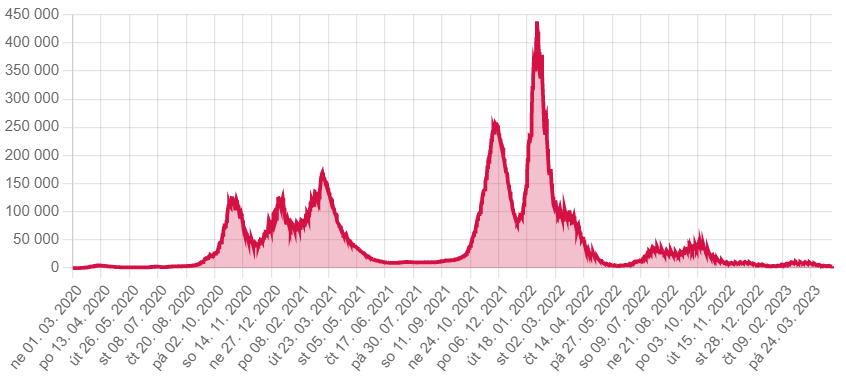
\includegraphics[width=1\textwidth]{Pictures/onemocneni.png}
	\caption{Přehled celkového počtu osob s~aktuálně probíhajícím onemocněním covid‑19\cite{onemocneni-aktualne}}
	\label{fig:SoucasnyCovid}
\end{figure}

Podle projektu OpenDataLab má ukončené očkování přes 6,8 miliónů lidí v~ČR, to činí přes 65\% obyvatel, celkový počet vydaných dávek přesahuje 18 miliónů. Celkový počet úmrtí v~ČR na toto onemocnění činí přes 42 tisíc \cite{soucasnystav-covid-statistika}.

Momentálně není v~České republice v~případě pozitivního výsledku testu automaticky nařizována karanténa. Izolace se nařizuje pouze v~situacích, kdy je to nutné pro zachování ochrany veřejného zdraví \cite{dopady-covid-izolace}. Omezení, která se vztahovala v~případě absence očkování, již neplatí. I~přesto, že již povinnost mít zakryté dýchací ústrojí respirátorem nebo rouškou není platná, stále se potkáte s~lidmi, kteří se pečlivě chrání.

\section{Současné aplikace}
\label{existing-apps}
Ministerstvo zdravotnictví poskytuje základní přehled o~dění v~souvislosti s koronavirem na svých online stránkách přes webovou aplikaci. Mimo jiné poskytuje i~webové API, které umožňuje vývojářům stahovat data.

\subsection{Webový portál MZČR}
MZČR má svůj vlastní webový portál na stránkách Onemocnění aktuálně \cite{onemocneni-aktualne}, který poskytuje informace o~stavu nemoci covid-19 v~České republice. Tento portál se nazývá Onemocnění aktuálně a~vznikl ve spolupráci s~ÚZIS ČR.

Ústav zdravotnických informací a~statistiky ČR je částí vlády, kterou zřizuje Ministerstvo zdravotnictví. ÚZIS ČR je správcem Národního zdravotnického informačního systému. Tento ústav spolupracuje s~Českým statistickým úřadem a~poskytovateli zdravotních služeb a~má vazby s~mnoha jinými zdravotnickými organizacemi jako jsou WHO, OECD, OSN a~EUROSTAT. Podle zákona je zdrojem oficiálních informací o~zdravotnické statistice pro Českou republiku \cite{uzis-definice}.

\subsubsection*{Hlavní stránka}

Hlavní stránka obsahuje přehled o~nemoci v~rámci celé ČR a~také řadu interaktivních grafů, které se dají měnit podle zvoleného časového rozmezí. Mezi informace, které grafy vyobrazují, patří např. přehled počtu osob s~nově prokázaným onemocněním covid-19 a~také přehled osob s~aktuálně probíhajícím onemocněním covid-19. Dále zde také najdete počty provedených PCR a~antigenních testů nebo i~přehled hospitalizací osob s~prokázaným onemocněním. Na hlavní stránce se nachází dvě interaktivní mapy, obě mapy vyobrazují výskyt laboratorně prokázaného onemocnění covid-19 s~tím rozdílem, že jedna z~nich zohledňuje kraje a~druhá okresy. Mapy vyobrazují jedinou informaci a~to celkový počet případů onemocnění za celé vaše zvolené období. 

\subsubsection*{Krajské zpravodajství}

Pokud bychom se chtěli dozvědět více informací o~krajích, webový portál nám umožňuje filtrovat data podle kraje. Na webové stránce se zvoleným krajem se vyskytují téměř totožné interaktivní grafy společně s podobnými přehledy, tentokrát pouze pro určitý kraj. Překvapí nás ale nové interaktivní mapy, v~tomto případě jsou dostupné tři a~mají rozšířenou funkčnost. I~přesto, že mapy vyobrazují celou ČR, tak se zobrazují hodnoty pouze v~okresech, které se nachází v~současně vybraném kraji. Tyto interaktivní mapy zobrazují denní přírůstky onemocnění, vyléčených osob a~také úmrtí. Barvy na mapě se škálují podle nejvyššího denního přírůstku v~rámci okresu za celé sledované období. Díky tomu lze na mapě spatřit tzv. covidové vlny. Má to ale i~svou nevýhodu, a~to, že mimo zmíněné covidové vlny jsou barvy na mapě těžce rozeznatelné. Bohužel nelze tyto mapy jinak přizpůsobit. Máme k~dispozici zvolení určitého dne a~spuštění animace, ale mapa nám nedovolí si zvolit určité období a~pohybovat se pouze v~daném období, tudíž by se nám barvy na mapě škálovaly odlišně. Proti tomuto se dá argumentovat, že by zobrazované hodnoty mohly být zkreslené, ale díky tomu můžeme naopak lépe pozorovat období mimo covidové vlny. Příklad mapy vyobrazující denní přírůstek onemocnění lze vidět na obrázku \ref{fig:OnemocneniAktualneScreen}.

\begin{figure}
	\centering
	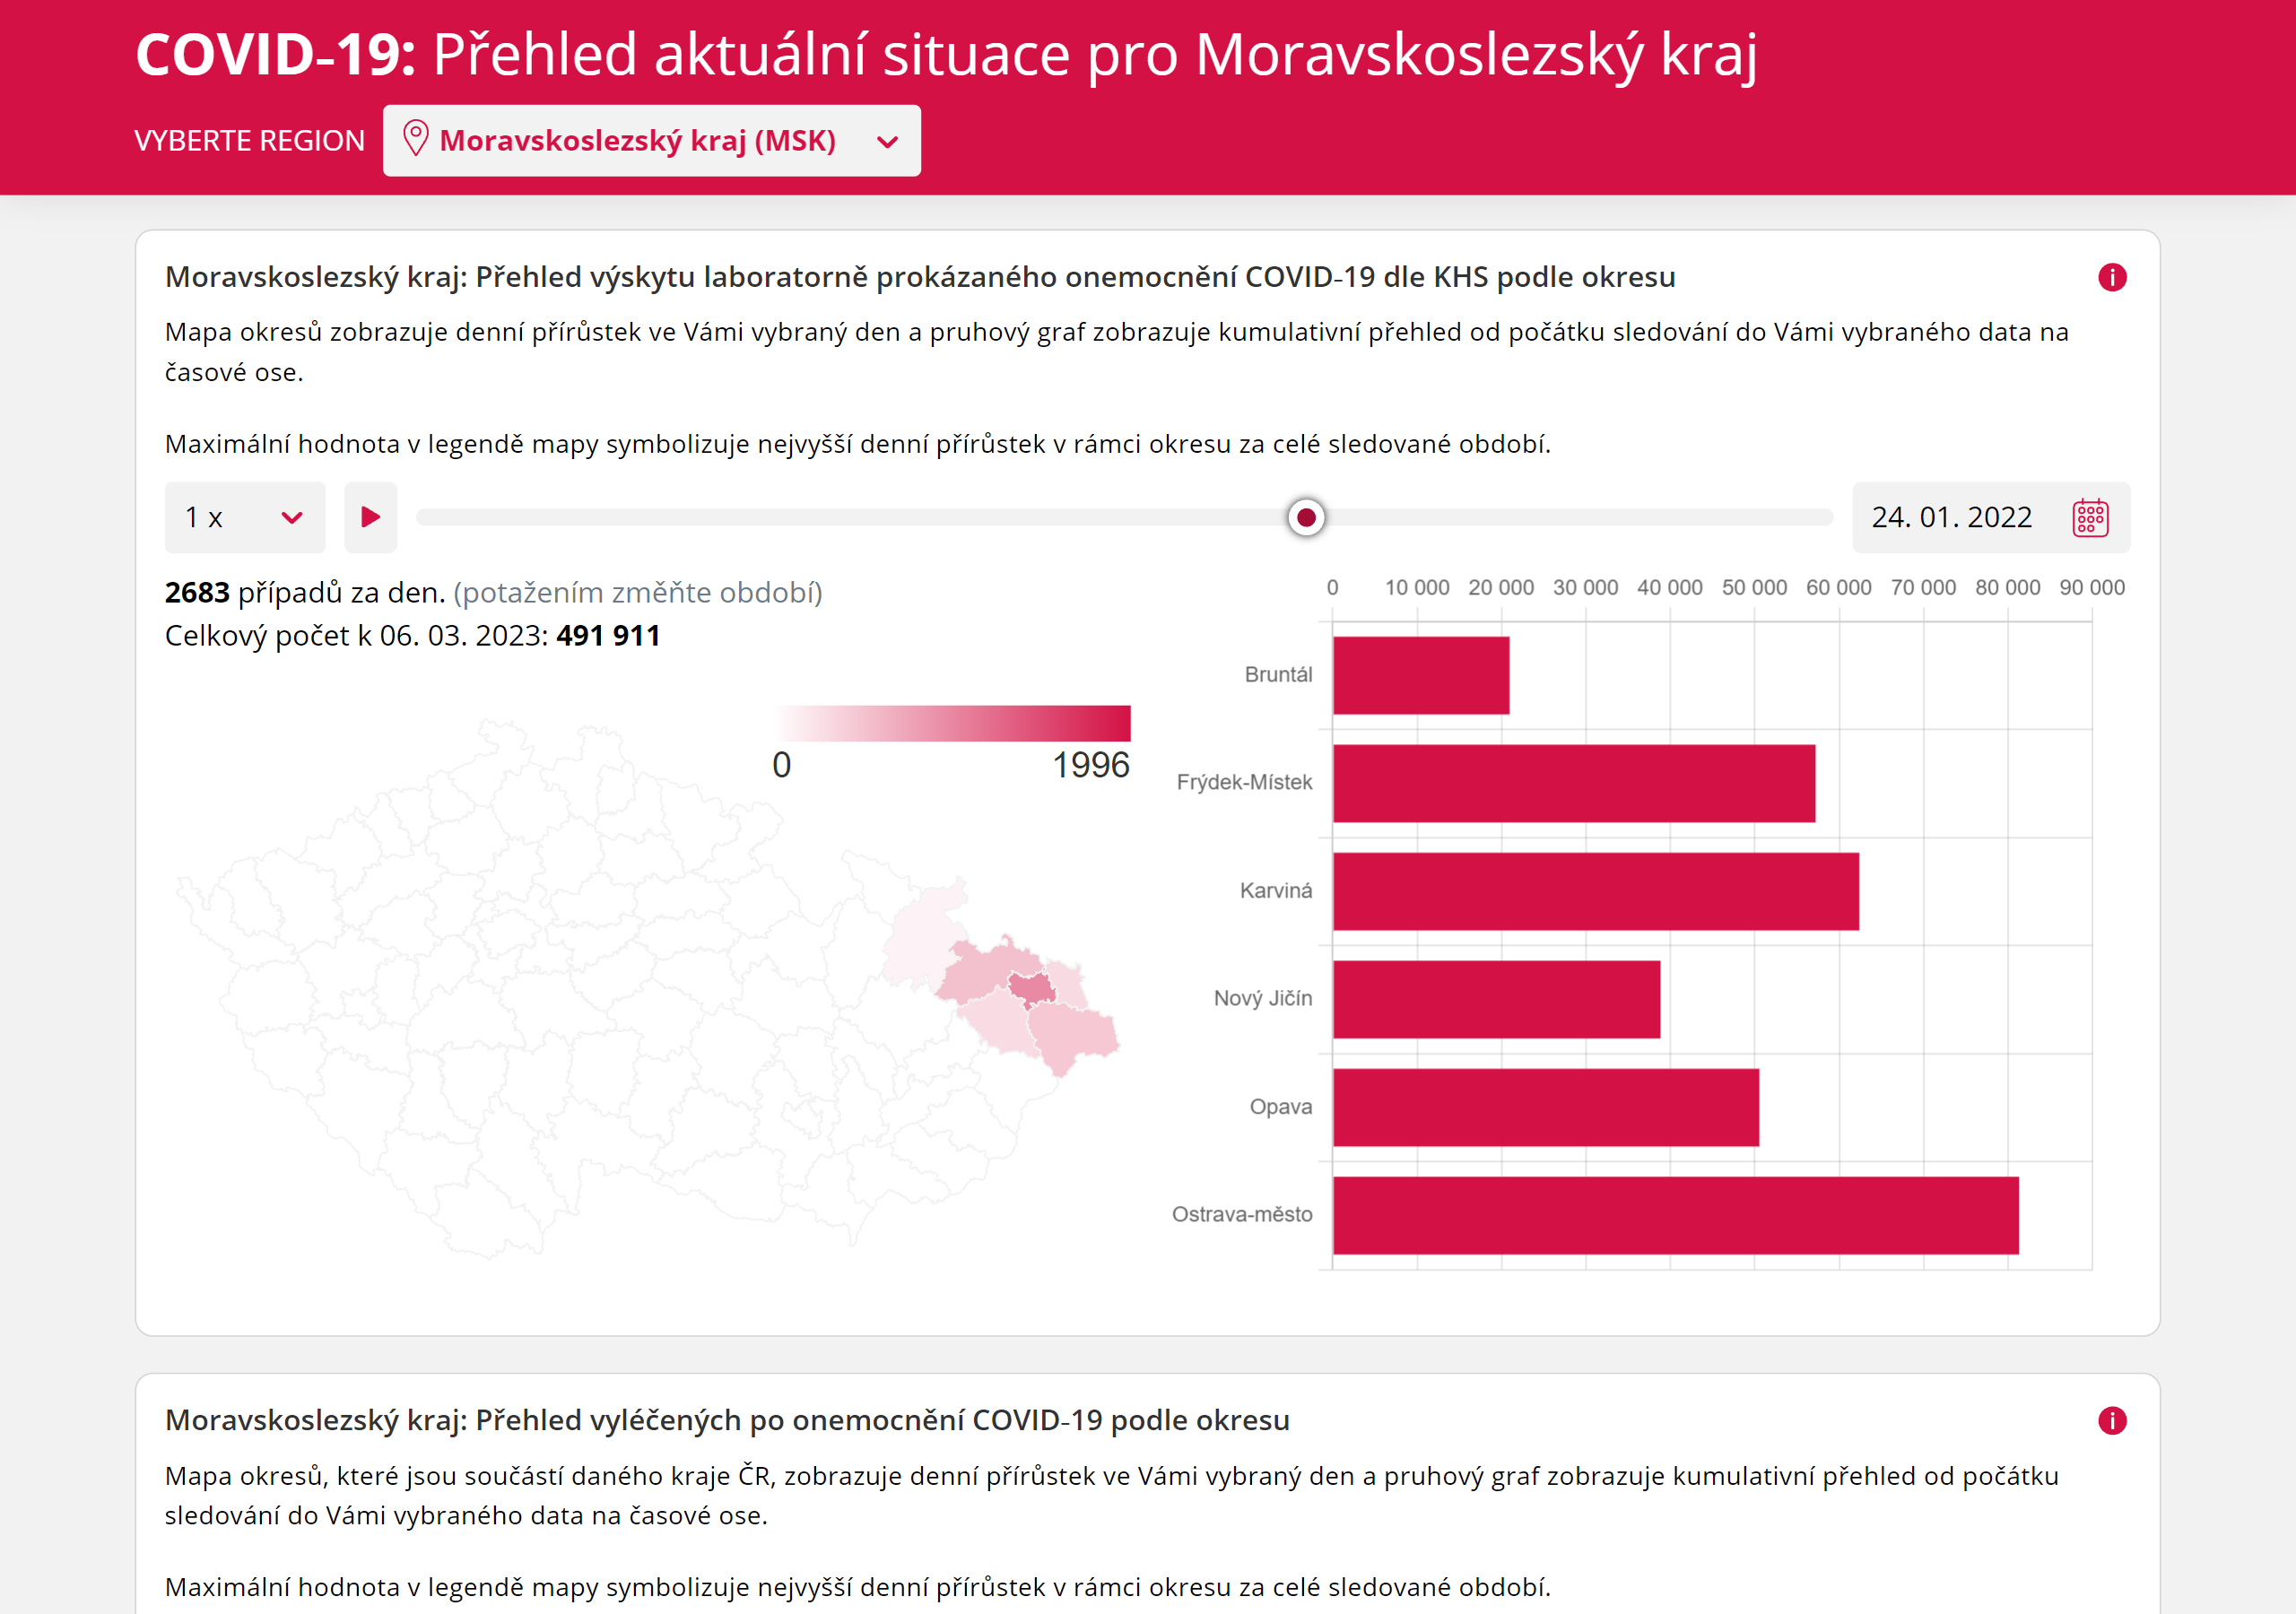
\includegraphics[width=0.8\textwidth]{Pictures/onemocneni-aktualne-screen.png}
	\caption{Vizualizace onemocnění v~aplikaci Onemocnění aktuálně v~Moravskoslezském kraji\cite{onemocneni-aktualne-msk}}
	\label{fig:OnemocneniAktualneScreen}
\end{figure}

\subsubsection*{Přehledy dle KHS}

Lepší přehled o~okresech lze nalézt v~záložce \emph{Přehledy dle KHS}. Na této stránce jsou funkčně totožné interaktivní mapy jako u~krajů s~tím rozdílem, že se na mapě ČR vyobrazují všechny okresy. Můžeme zkoumat data denních přírůstků infekcí, vyléčení a~úmrtí, ale stejně jako u~krajů si nemůžeme mapu nijak přizpůsobit. Opět se barvy na mapě škálují podle nejvyššího denního přírůstku v~rámci okresu za celé sledované období.

Ideální interaktivní mapa by zobrazovala všechny okresy na jedné mapě ČR s~možnostmi přizpůsobení období a~škálování, takovou mapu v~této webové aplikaci nenajdeme.

\subsection{OpenDataLab}
Projekt OpenDataLab vznikl ve spolupráci s~Fakultou informačních technologií ČVUT v~Praze a~společností Profinit EU. Jedná se o~otevřenou laboratoř určenou hlavně pro studenty. Jejich hlavním cílem je nabídnout nápady, pomoc a~případně i~zadání semestrálních a~závěrečných prací studentům, jejich práce vytvořené pro školu jsou veřejné a~slouží k~dobrému účelu \cite{opendatalab}.

Jedním z~jejich realizovaných projektů je web poskytující především statistická data o~jednotlivých očkovacích místech, jejich dostupnosti, zaplněnosti a~celkových statistikách o~daném místě. Očkovací místa se dají roztřídit podle krajů nebo typu vakcíny, takže se v~datech neztratíte. Aplikace také umožňuje místa filtrovat detailněji, např. podle věku, zda je nutno se na daném místě registrovat nebo zda je dané místo i~pro samoplátce. U~každého očkovacího místa se dozvíte kolik lidí je právě rezervovaných a~u~některých se i~dozvíte průměrnou dobu čekání na rezervaci.

Mimo vyhledávání očkovacích míst zahrnuje tento web souhrnné statistiky o~koronaviru a~očkování v~ČR. Na této stránce vás uvítá rozsáhlá tabulka dat, která zahrnuje mnoho informací o~očkování např. počtu rezervací na očkování, vydaných dávek nebo počet lidí čekajících ve frontě. 

\begin{figure}[h]
	\centering
	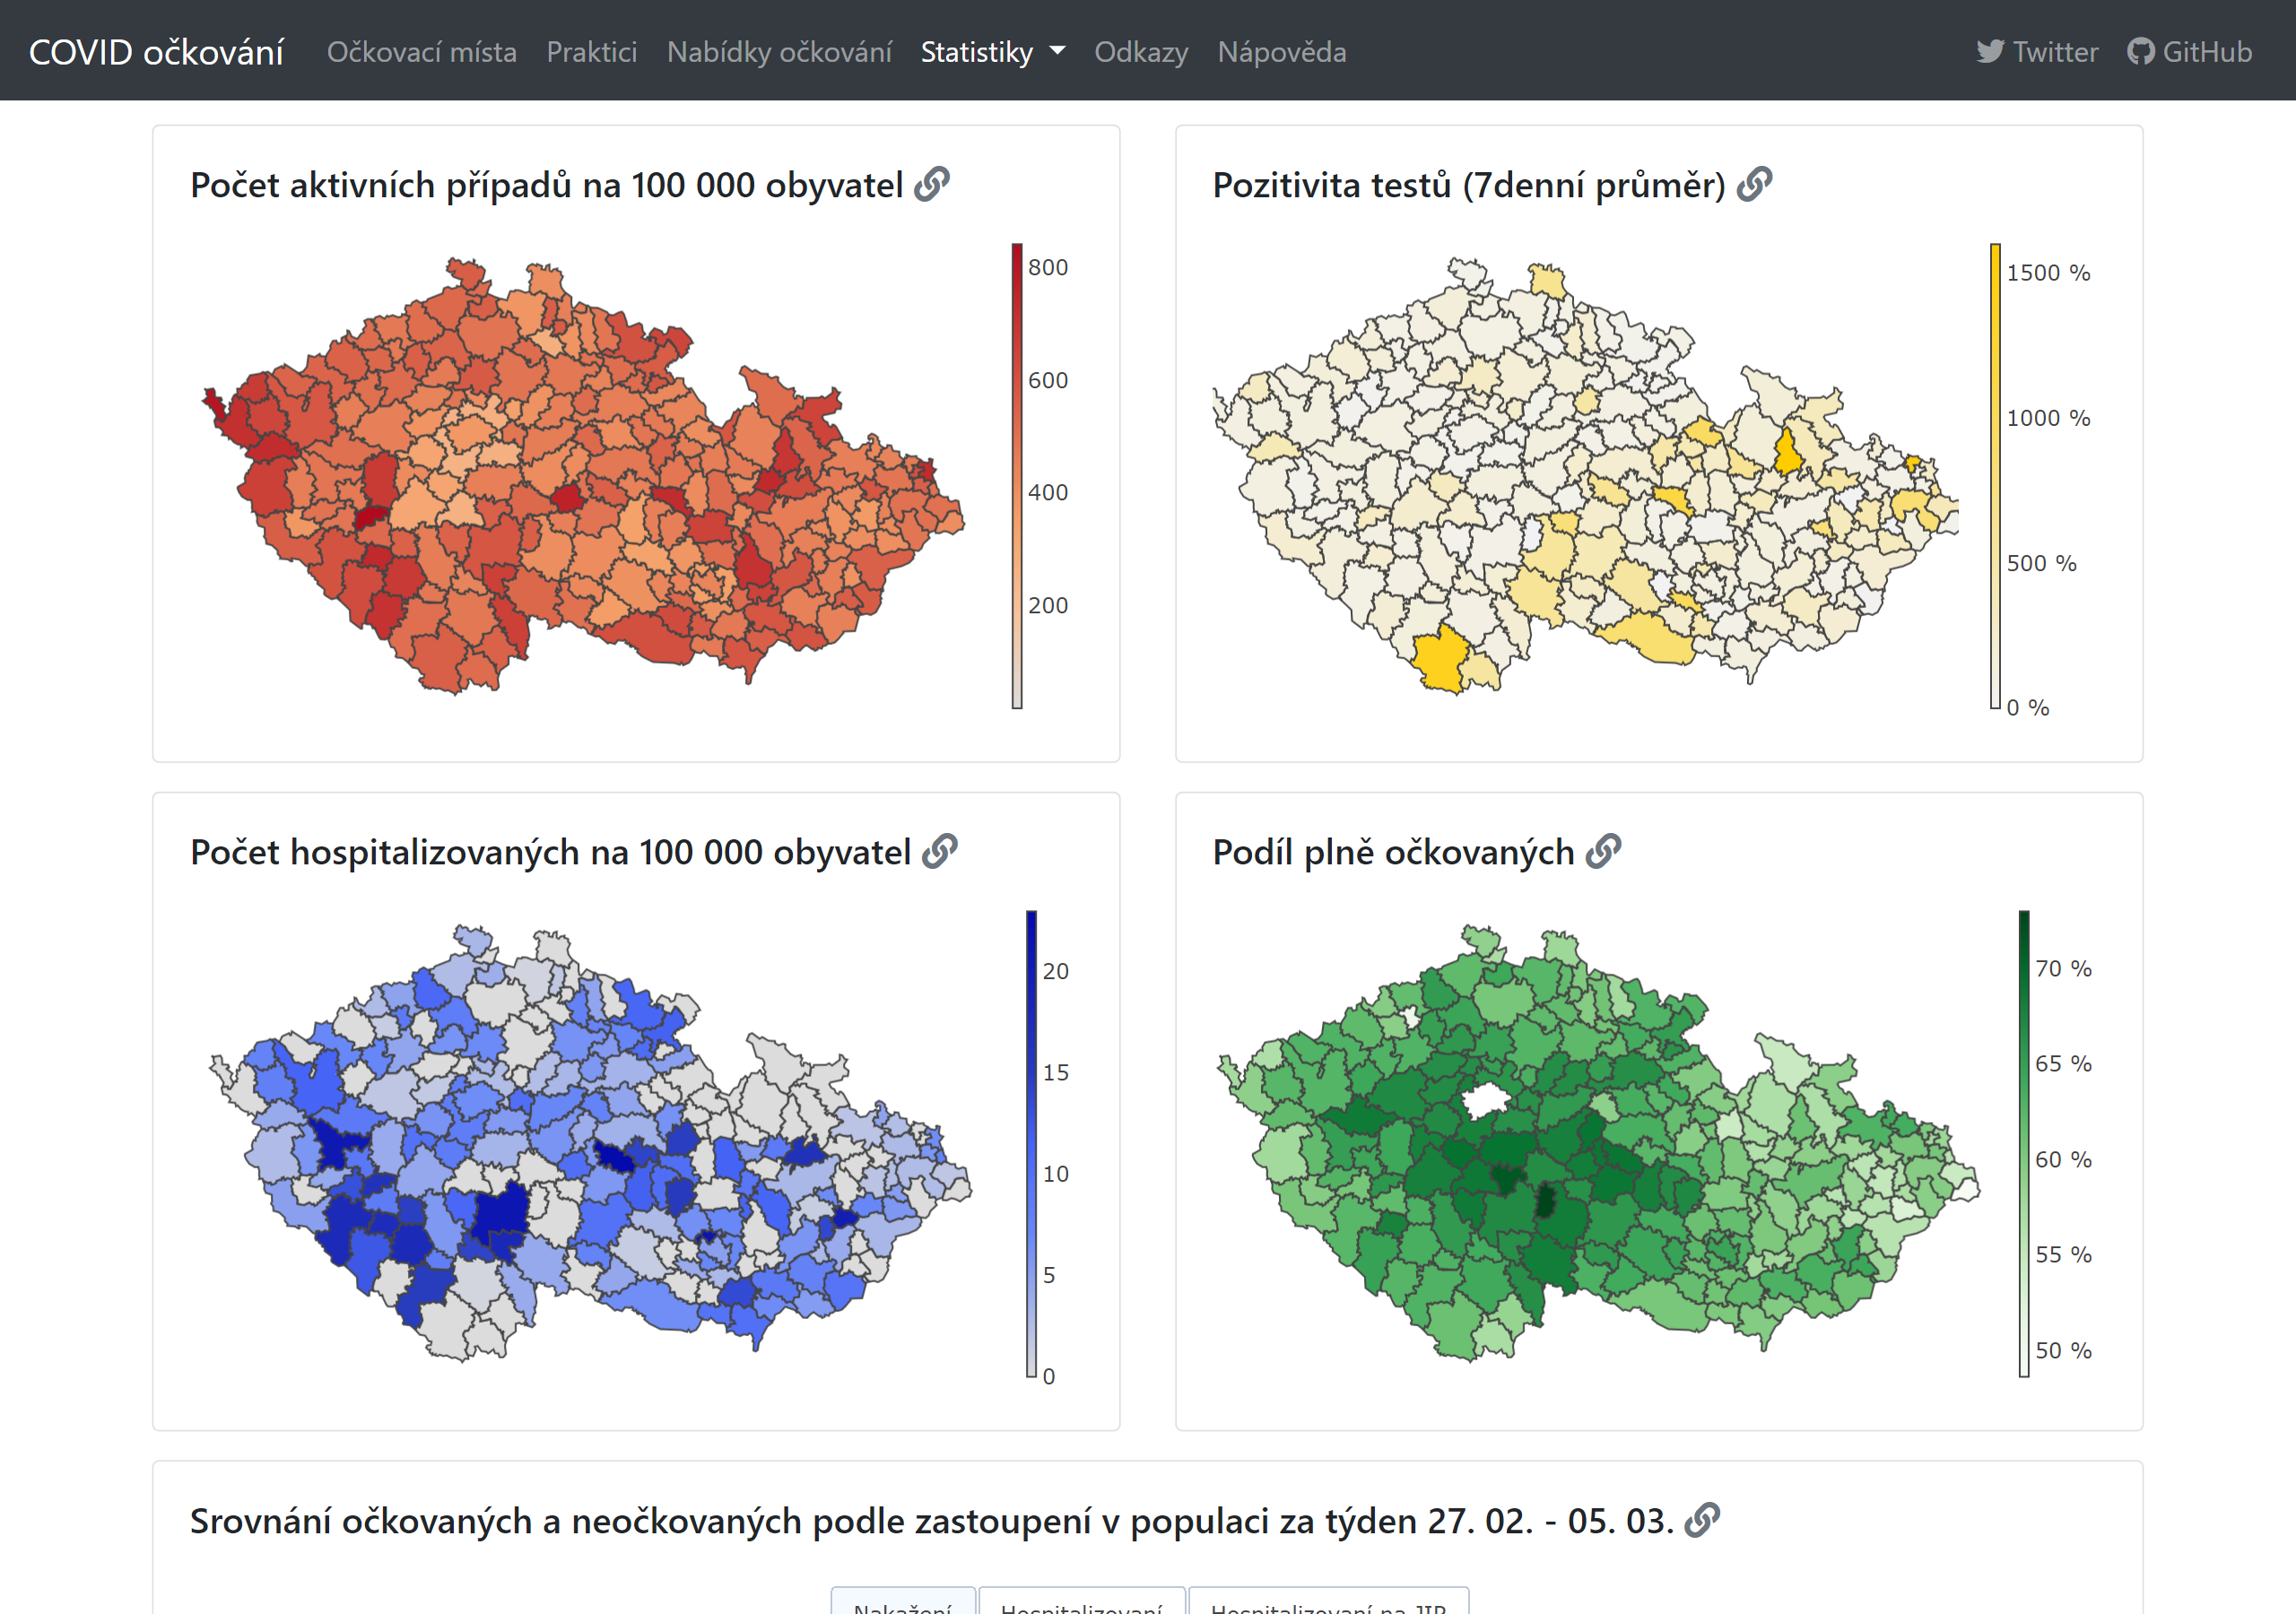
\includegraphics[width=1\textwidth]{Pictures/opendatalab-screen.png}
	\caption{Vizualizace onemocnění v~aplikaci projektu OpenDataLab \cite{soucasnystav-covid-statistika}}
	\label{fig:OpenDataLabScreen}
\end{figure}

Součástí statistik jsou i~souhrnné mapy, které vyobrazují současný stav z~hlediska aktivních případů, pozitivity testů, počtu hospitalizovaných a~plně očkovaných. Tyto mapy nejsou nijak přizpůsobitelné a~nelze si je omezit na určité období. Nejdůležitější část této statistiky jsou interaktivní grafy, které jsou zaměřené na vývoj počtu očkovaných, registrací, front a~nebo také na porovnání různých typu vakcín. Zmíněné mapy lze spatřit na obrázku \ref{fig:OpenDataLabScreen}.

Tuto webovou aplikaci lze nalézt na stránkách OpenDataLab \cite{opendatalab-ockovani}.

\section{Dostupná data}

\subsection{O~dostupných datech}
Data o~počtech ovlivněných koronavirovým onemocněním mohou být získávána z~různých zdrojů. WHO (\emph{World Health Organization}) poskytuje data na celosvětové úrovni, ECDC (\emph{European Centre for Disease Prevention and Control}) pro Evropu a~CDC (\emph{Centers for Disease Control and Prevention}) pro Spojené státy americké. V~rámci jednotlivých zemí poskytují regionální data ministerstva zdravotnictví. V~ČR jsou data dostupná veřejnosti v~datových sadách, které spravuje MZČR \cite{bednarkova-covid}.

\subsection{Onemocnění aktuálně API v3}
\label{sec:onemocneni-aktualne}
Součástí webového portálu Onemocnění aktuálně jsou i~otevřené datové sady zdarma ke stažení obsahující širokou škálu dat o~onemocnění covid-19. Existuje několik verzí těchto datových sad, starší verze jsou zprostředkovány jako rozsáhlé datasety ve formě CSV. Pracovat budeme s~nejnovější verzí 3, která je zprostředkována jako webové API.

API je zkratkou pro aplikační programovací rozhraní. Jedná se o~rozhraní, které poskytuje řadu funkcí, jež umožňují programátorovi přistoupit k~určitým datům nebo funkcím aplikace. V~podstatě se jedná o~způsob, jakým aplikace mezi sebou komunikují, aby mohly sdílet data a~funkce \cite{api-definice}. Webové API je takové API, ke kterému je možné přistoupit prostřednictvím webu.

K~dispozici je široká škála dat, avšak pouze část těchto dat zohledňuje okresy ČR. Zde je seznam datasetů, které byly využity při tvorbě aplikace, a jaká data byla z těchto datasetů použita:
\begin{itemize}
    \item \emph{obce} (informace o~případech infekce v~obcích),
    \item \emph{ockovani-geografie} (informace o~vydaných dávkách očkování v~krajích s~bydlišti osob na úrovni ORP),
    \item \emph{umrti} (informace o~nových úmrtí v~okresech),
    \item \emph{kraj-okres-testy} (informace o~provedených PCR testech v~okresech).
\end{itemize}

Všechny zmíněné datasety kromě \emph{ockovani-geografie} obsahují informace na úrovni okresů. Pouze u~datasetu \emph{ockovani-geografie} je potřeba zařadit ORP do okresu. Dataset obsahuje informace o~vydaných dávkách očkování v~daném kraji s~bydlištěm očkované osoby na úrovni ORP. Aplikace tudíž bude vyobrazovat počet vydaných dávek na základě bydlišť osob, takže vyobrazené informace nemusí být zcela přesné.

Je důležité zmínit, že poskytovaná data se neustále mění. Dochází tak k~nepřesnostem při snaze zvizualizovat brzká data, proto je doporučeno 
se na tato data nespoléhat a~vyčkat několik dní nebo i~týdnů, než se data zaktualizují na přesnější hodnoty.

Každý záznam poskytovaný tímto API má přiřazený svůj identifikační řetězec, pomocí kterého se dá nalézt a~získat určitý záznam. Veškerá dokumentace k~tomuto API je dostupná na stránkách Onemocnění aktuálně \cite{onemocneni-aktualne-docs}.

\subsubsection*{Získání dat}

Data jsou volně přístupná komukoli, jediným požadavkem je registrace na portálu Onemocnění aktuálně. Po registraci získáte vlastní token, pomocí kterého je komunikace s~API zabezpečena. Token je při komunikaci s~API potřebný, při pokusu o~komunikaci bez tokenu vám API žádná covidová data nevrátí, pouze vás upozorní na absenci tokenu.

Pro získání dat z~API MZČR je potřeba zaslat dotaz na API ve formě HTTP požadavku. Požadavek musí obsahovat platný token a~také platnou URL adresu, která definuje typ žádaných dat. URL adresa může obsahovat různé parametry, např. omezení počtu výsledků, číslo stránky, omezení časového rozsahu nebo zvolení konkrétního okresu. Limit počtu dotazů každého uživatele je stanoven na 1000/hod. V~kódu \ref{src:PythonListing} je příklad pro získání dat z~API v~jazyce Python, přesněji získání kumulativních počtů souvisejících s~nemocí v~okrese Ostrava-město dne 5. ledna 2023:


\begin{lstlisting}[language=Python,label=src:PythonListing,caption={Zaslání HTTP požadavku v~jazyce Python}]
from urllib import request

url = 'https://onemocneni-aktualne.mzcr.cz/api/v3/kraj-okres-nakazeni-vyleceni-umrti?page=1&itemsPerPage=100&datum%5Bbefore%5D=2023-01-05&datum%5Bafter%5D=2023-01-05&okres_lau_kod=CZ0806&apiToken=xyz'
req = request.Request(url)
req.add_header('accept', 'application/json')
response = request.urlopen(req)

\end{lstlisting}

\subsubsection*{Formát dat}
API verze 3 nám umožňuje vyžádat si různý formát dat výsledku. Hodnotu výsledku to neovlivní, pouze se změní formátování vráceného dokumentu. Pro vyžádání určitého formátu stačí do HTTP požadavku vložit hlavičku \emph{accept} s~hodnotou daného formátu. K~dispozici máme čtyři možnosti:

\begin{itemize}
    \item application/ld+json (formát JSON-LD),
    \item application/json (formát JSON),
    \item text/html (formát HTML),
    \item text/csv (formát CSV).
\end{itemize}

Příklad formátování je k~dispozici v~kódu \ref{src:JavaListing}, kde se nachází vrácený výsledek Python kódu \ref{src:PythonListing} s~vyžádaným formátem application/json:

\begin{lstlisting}[language=Java,label=src:JavaListing,caption={Příklad vráceného výsledku API}]
[
  {
    "id": "8ed855a3-35c6-40c3-8a8f-7cf4ddd169d5",
    "datum": "2023-01-05",
    "kraj_nuts_kod": "CZ080",
    "okres_lau_kod": "CZ0806",
    "kumulativni_pocet_nakazenych": 131424,
    "kumulativni_pocet_vylecenych": 130766,
    "kumulativni_pocet_umrti": 1434
  }
]

\end{lstlisting}

Vrácená data jsou ve vyžádaném JSON formátu, s~tímto formátem bude aplikace pracovat. JSON je zkratka pro \emph{Java Script Object Notation}, jedná se o~odlehčený formát pro výměnu dat, který je snadno srozumitelný. JSON je textový formát, který je zcela nezávislý na jazyku, ale používá konvence, které jsou známé programátorům jazyků jako jsou C++, C\#, Java, JavaScript, Python a~mnoho dalších \cite{json-definice}.

Při požádání o~data nám toto API vrátí výsledek, který je sestupně setřízený podle dní. Pokud obsahuje výsledek i~identikační kódy, jako např. NUTS kód nebo LAU kód, bývá tento výsledek sestupně setřízený i~podle těchto kódů.

\subsection{Pomocná data ČSÚ}
\label{csu}
Při práci s~daty ÚZIS a~MZČR budou potřeba dodatečná data, která jsou dostupná online na stránkách Českého statistického úřadu. Bude potřeba identifikovat okresy a~obce podle jejich identifikačních kódů, zařadit ORP do okresů a~také bude potřeba znát počty obyvatel v~okresech pro přepočty hodnot.

\subsubsection*{Seznam okresů a~jejich identifikace}

Pokud žádáme zmíněné API o~data, která jsou spojena s~kraji, okresy nebo obcemi, obsahují tato data identifikátory, které definují o~jaký územní celek se jedná. MZČR pracuje ve svém API s~identifikačními NUTS kódy a~LAU kódy.

Klasifikace NUTS (\emph{Nomenclature of territorial units for statistics}) je systém, který slouží k~rozdělení ekonomického území Evropské unie a~Spojeného království na různé úrovně. Cílem tohoto systému je získávat statistická data a~socioekonomické informace o~jednotlivých regionech. Klasifikace NUTS obsahuje více úrovní, které umožňují podrobnější rozdělení regionů:

\begin{itemize}
    \item NUTS 1: nejvyšší úroveň regionů - celé území ČR,
    \item NUTS 2: regiony druhé úrovně - regiony (např. Moravskoslezsko, Střední Čechy nebo Jihovýchod),
    \item NUTS 3: malé regiony - kraje ČR \cite{europa-eu-nuts}.
\end{itemize}

LAU (\emph{Local administrative unit}) je systém, který byl vytvořený EU pro identifikaci územních jednotek v~Evropě. Oproti NUTS, který se používá na regionální evropské úrovni, se LAU používá na místní úrovni. Používá se také pro statistické účely jako např. pro sběr a~analýzu dat v~oblastech demografie, hospodářství a~jiné. Tyto jednotky se považují za stavební jednotku NUTS systému a~v~ČR se řadí do dvou úrovní:

\begin{itemize}
    \item horní úroveň LAU 1 - okresy,
    \item spodní úroveň LAU 2 - obce \cite{csu-lau}.
\end{itemize}

Rozdělení České republiky na NUTS 3 (kraje) a~LAU 1 (okresy) lze vidět na obrázku \ref{fig:NutsLau}. Obrázek pochází z~webu ČSÚ \cite{nuts-lau-pic}.

\begin{figure}[h]
	\centering
	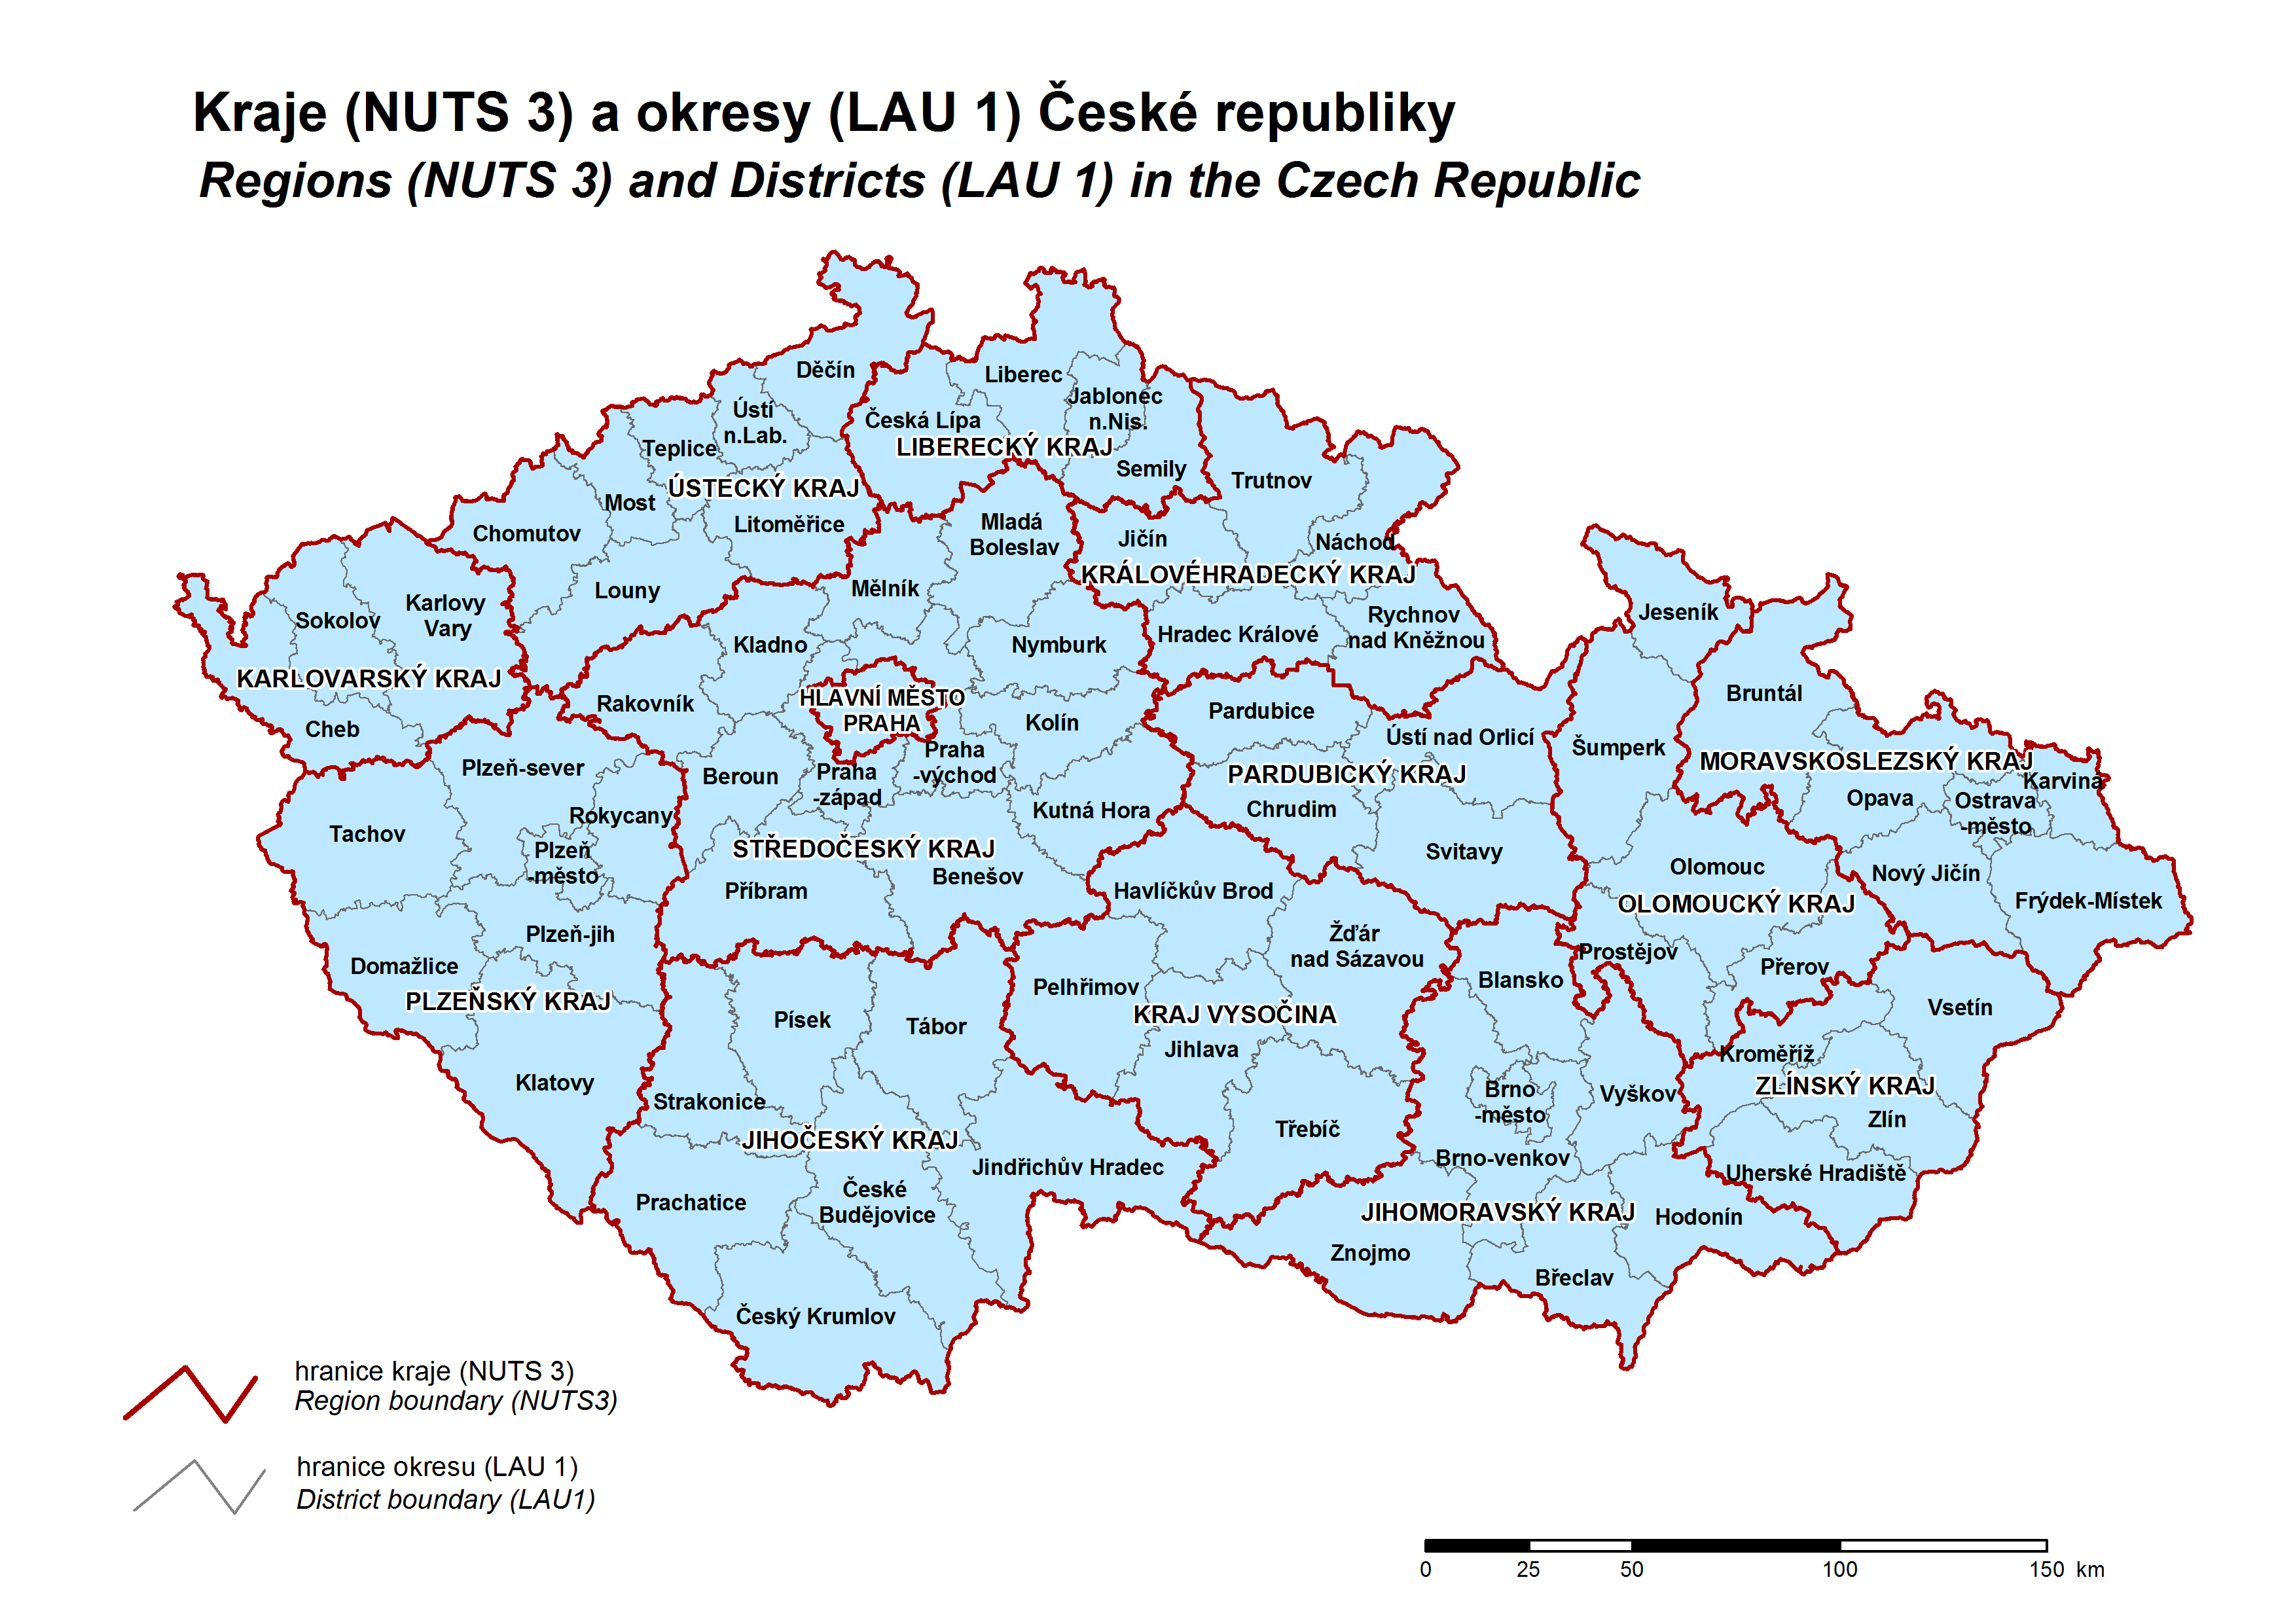
\includegraphics[width=1\textwidth]{Pictures/nuts_lau.png}
	\caption{Rozdělení České republiky na NUTS 3 a~LAU 1 \cite{nuts-lau-pic}}
	\label{fig:NutsLau}
\end{figure}

Vzhledem k~tomu, že je práce zaměřena na okresy ČR, budou se využívat pouze LAU kódy. Abychom mohli ve výsledcích API rozpoznat o~který okres se jedná, potřebujeme číselník, který nám umožní identifikovat daný LAU kód. Český statistický úřad poskytuje tento číselník online na stránkách ČSÚ \cite{czso-ciselnik-lau}. Číselník je možné stáhnout v~několika formátech, např. v~XML nebo CSV.

\subsubsection*{Zařazení ORP do okresů}
\label{sec:ciselnik-orp}

Práce bude využívat dataset s~informacemi o~vydaných dávkách očkování. Obsažená data nesou informaci o~bydlišti osoby, které byla vydaná jedna z~dávek. Bydliště je na úrovni ORP (obec s~rozšířenou působností) a~je nutné ji přiřadit okres, ve kterém se nachází. To umožní číselník na stránkách ČSÚ \cite{csu-ciselnik-orp}, který obsahuje potřebné informace k~přiřazení ORP do okresů.

\subsubsection*{Počet obyvatel v~okresech}

Při vizualizaci dat se bude pracovat i~s~přepočtem na sto tisíc obyvatel, který se běžně používá ve statistice. Jedná se o~hodnotu, která může přesněji vyobrazit situaci v~daném okrese. ČSÚ poskytuje své výsledky sčítání lidu na svých stránkách \cite{czso-pocet-obyvatel}. Data poskytuje ve formátu CSV a~obsahují velkou řadu informací, obsahuje nejen počty obyvatel v~krajích a~okresech rozdělené podle pohlaví, ale třeba i~průměrný věk podle pohlaví v~těchto celcích. Data byla přeformátována tak, aby byla jednoduše použitelná v~naší aplikaci.

\endinput
\chapter{Analýza řešení}

\section{Cíl a~schopnost nového řešení}

Po zkoumání současných dostupných aplikací se zjistilo, že žádné z~těchto řešení není na vizualizaci dat o~koronaviru na úrovni okresů ideální. Aplikace Onemocnění aktuálně poskytuje několik interaktivních map na úrovni okresů, ale žádná z~těchto map není schopna dostatečného přizpůsobení nebo zobrazují pouze část ČR. Naopak aplikace projektu OpenDataLab poskytuje takové mapy, které vyobrazují pouze současnou situaci, takže se v~nich nelze posouvat v~čase. Tyto mapy nejsou nijak přizpůsobitelné.

Ideální aplikace by byla taková, která by poskytovala plně interaktivní mapu okresů ČR a~kterou by si mohl uživatel libovolně přizpůsobit ať už z~hlediska dat, času nebo vzhledu. Toto umožní uživateli si aplikaci přizpůsobit právě svému použití a~zpříjemnit mu průběh používání. Vše, co musí výsledná aplikace splňovat a~čeho bude aplikace schopna, je shrnuto v~následujícím seznamu:

\begin{itemize}
    \item musí obsahovat mapu ČR s~rozdělením na okresy,
    \item obsažená mapa musí obsahovat interaktivní prvky (např. po kliknutí nebo přejetí myší po okrese zobrazit dodatečné informace),
    \item schopnost zobrazit průběh koronaviru po celé období zkoumání,
    \item schopnost zkoumat daná období (např. konkrétní covidové vlny),
    \item schopnost vyobrazit všechny čtyři datasety (infekce, úmrtí, očkování, PCR testy),
    \item možnost porovnat různé datasety v~reálném čase a~umožnit tak uživateli najít souvislosti,
    \item možnost spuštění animace (automatické posouvání data),
    \item možnost si mapu přizpůsobit dle potřeb (např. průhlednosti vrstev nebo přiblížení),
    \item schopnost ukládat covidová data na serveru aplikace, aktualizovat je a~poskytovat je uživateli.
\end{itemize}

Pokud by byla aplikace v~budoucnu nasazena na veřejný server, dá veřejnosti nový pohled na průběh koronaviru v~České republice. Aplikace bude využitelná v~mnoha oblastech, umožní lidem pohlédnout zpět do historie průběhu koronaviru a~získat tak potřebné informace. Díky schopnosti porovnávat data v~reálném čase mohou uživatelé snadno hledat souvislosti mezi různými daty a~zjistit tak zajímavé poznatky. Uživatel se bude moci stát režisérem a~společně se svými vybranými daty a~přizpůsobením mapy dokáže vytvořit pozoruhodné animace. 

\section{Rozbor možných způsobů řešení}
Ještě několik desetiletí zpátky existovaly pouze takové primitivní počítače, které byly sestaveny na určitou činnost a~nenabízely uživateli tolik možností jako dnes. Pojem internet nikdo neznal a~představa chytrého telefonu, který vás bude navigovat ve městě, byl pouhý sen každého člověka. V~dnešní moderní době jsou taková zařízení a~možnosti zcela běžné a~někteří z~nás si bez nich nedokážou představit svůj život. Díky těmto novým technologiím nejsou aplikace stavěné pouze na stolní počítače, jak tomu bývalo v~historii, ale i~na mobilní zařízení. Nově lze také vyvíjet takovou aplikaci, která pracuje pouze ve webovém prohlížeči. U~takových aplikací se musí dbát na nové požadavky jako např. vyžadovat připojení k~internetu nebo optimalizovat aplikaci tak, aby nevybíjela moc baterie. Aplikace lze tedy psát na několik platforem, např. na stolní počítače, mobilní zařízení nebo na web.

Rád bych tyto typy aplikací porovnal, poukázal na jejich výhody a~nevýhody a~poté zvolil nejvhodnější typ pro naše využití.

\subsection{Desktopová aplikace}
Desktopové aplikace jsou software, který lze spustit lokálně na osobních počítačích. Mezi takové počítače můžeme řadit např. stolní počítače nebo přenosné notebooky. Osobní počítače mají podobné vlastnosti, téměř všechny se ovládají myší a~klávesnicí, mají velké obrazovky (oproti mobilním zařízením) a~často obsahují výkonný hardware. V~porovnání s~webovými aplikacemi není nutné, aby desktopové aplikace vyžadovaly internetové připojení k~jejich užití. Nevýhodou většiny desktopových aplikací je jejich neschopnost udržet se aktuální, tudíž se samovolně aktualizovat. Aktualizace aplikací často vyžadují nějakou interakci uživatele nebo i~zvýšená práva. Většina aplikací se také musí instalovat.

Všechny aplikace stavěné na desktop nejsou univerzální, mohou ale být kompatibilní v~různých verzích daného operačního systému. Příkladem může být aplikace vyvinutá pro operační systémy Windows, která nebude nativně spustitelná na systémech MacOS. Dominantním desktopovým operačním systémem na trhu je Windows společnosti Microsoft, který převažuje v~70 \% počítačích využívající desktopový OS \cite{marketshare-desktop-os}. Na grafu \ref{fig:MarketshareDesktopOS} lze vidět podíl desktopových OS na trhu od začátku roku 2022 do začátku roku 2023.

Otázkou je, zda je desktopová aplikace vhodná pro naše využití. Komplexní desktopové aplikace dokážou využít veškeré zdroje osobních počítačů při plnění náročnějších úkolů. V~našem případě se nejedná o~nijak hardwarově náročnou aplikaci, která by vyžadovala velký počet hardwarových prostředků. S~desktopovou aplikací nebude možné oslovit široké spektrum veřejnosti z~důvodu nemožnosti spustit aplikaci na všech operačních systémech. Někteří uživatelé také nemusí mít na svých zařízeních dostatečná práva k~instalaci aplikace.

% obrazek 14x21 cm
\begin{figure}
	\centering
	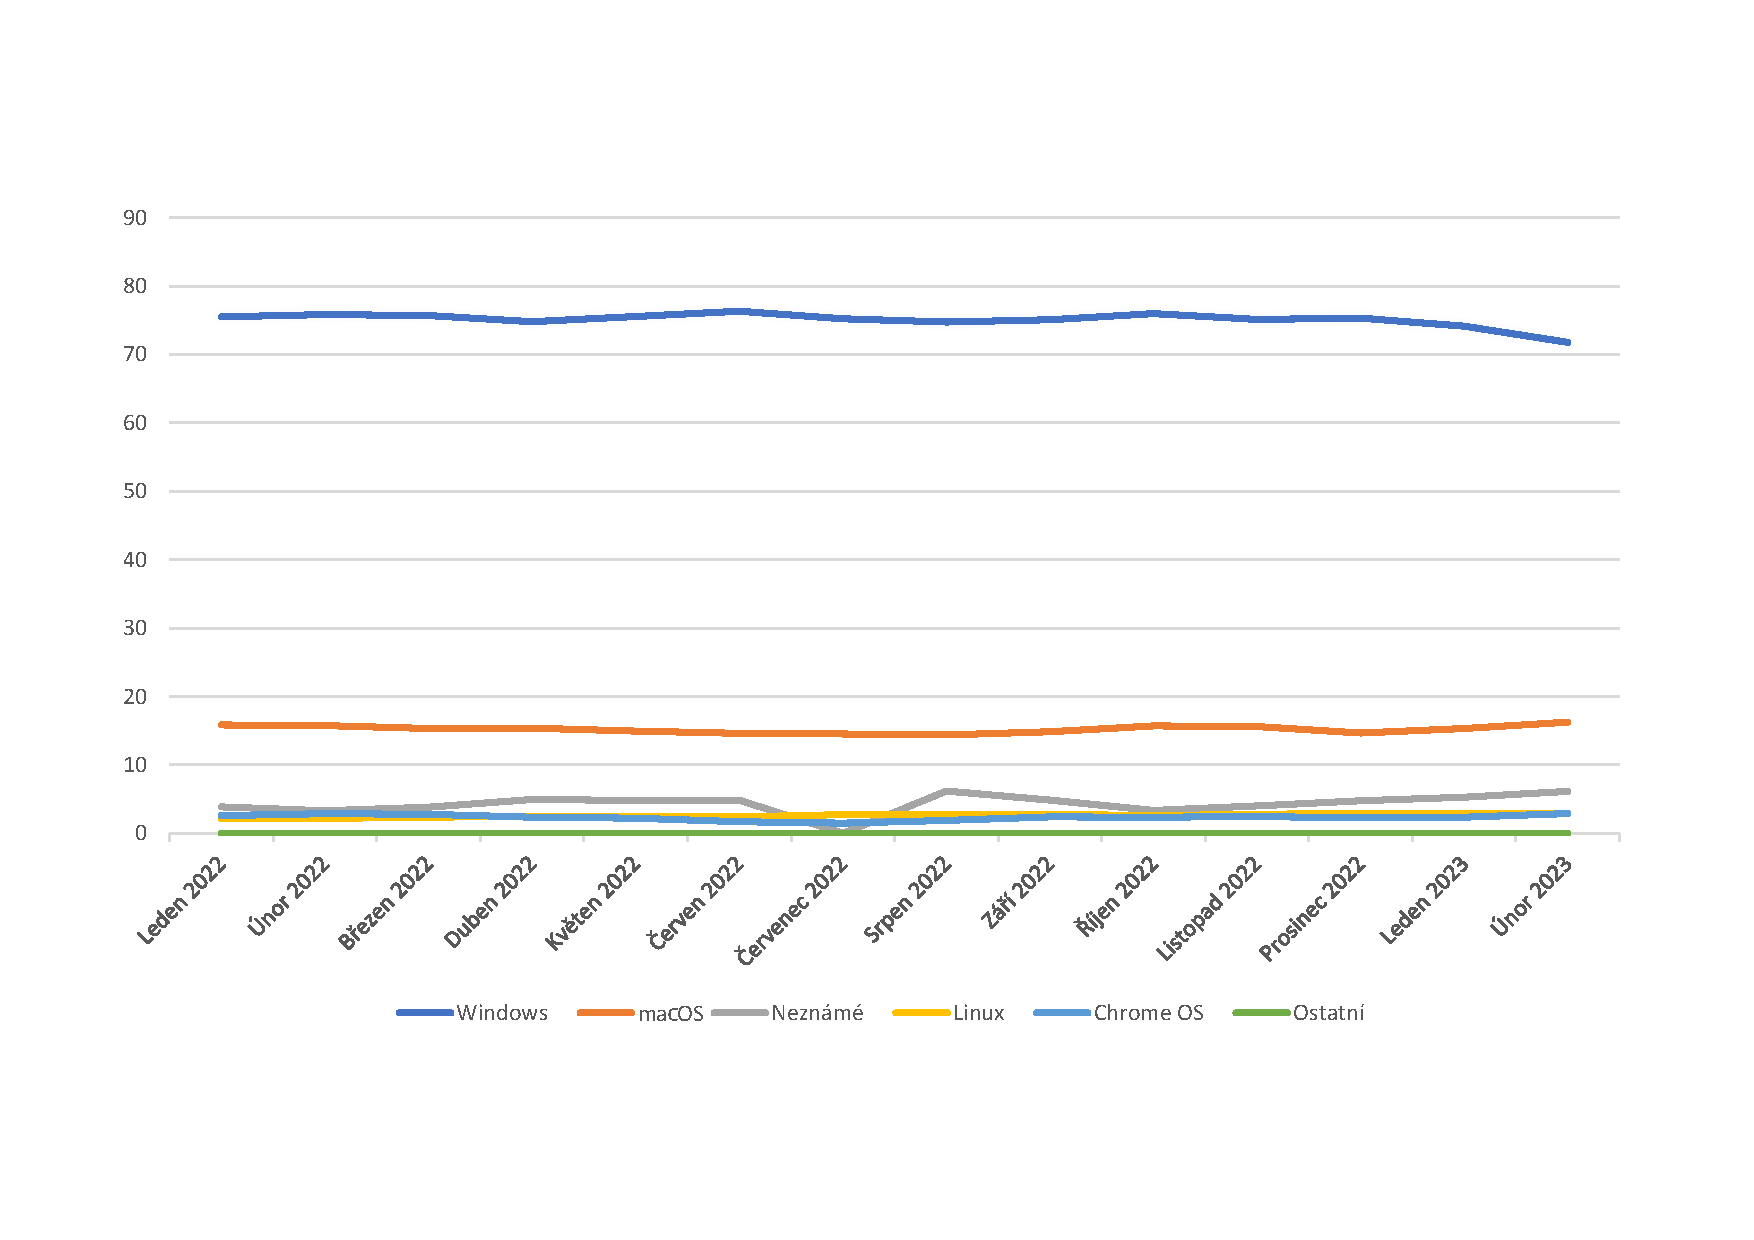
\includegraphics[width=1\textwidth]{Pictures/graf1.pdf}
	\caption{Podíl desktopových OS na trhu (v~\%) \cite{marketshare-desktop-os}}
	\label{fig:MarketshareDesktopOS}
\end{figure}

\subsection{Mobilní aplikace}

Mobilní aplikace jsou takový software, který lze vidět jako kontrast k desktopovým aplikacím. Jsou stavěné pro zařízení s~menšími obrazovkami, bezdrátovým připojením a~napájením z~baterie. V~dnešní době se jedná především o~chytré telefony a~tablety, chytré hodinky nebo např. i~software v~moderních automobilech. Takový software obsahuje různé optimalizace, aby předcházel nadměrnému vybíjení baterie, neboť baterie v~těchto zařízeních nemají vysoké kapacity. Většina těchto zařízení obsahuje dotykové obrazovky pomocí kterých může uživatel komunikovat s~technologií.

Mobilní aplikace jsou stavěné na menší obrazovky, tudíž nemají příliš prostoru na vyobrazování informací - je potřeba zobrazovat pouze ty informace, se kterými uživatele právě pracuje. Toto může být kámen úrazu pro naše využití - vizualizaci onemocnění na mapě ČR. Mapa ČR je vcelku rozsáhlá a~samotná mapa zabere na obrazovce hodně prostoru. Kdybychom chtěli v~aplikaci zobrazovat i~další elementy s~mapou jako např. informace o~zvoleném okrese, dodatečné grafy nebo nastavení, z~obrazovky by se zkrátka stal chaos. Řešením by mohly být chytré tablety, ale tato zařízení mají oproti chytrým telefonům podíl na trhu pouhých 3 až 4 \% \cite{marketshare-mobile-tablet}.

Podobně jako u~desktopových aplikací je nutné aplikaci stavět pro určitý mobilní operační systém neboť tyto systémy nejsou mezi sebou kompatibilní. Mezi nejpoužívanější mobilní OS patří Android společně s~iOS, kde Androidu náleží podíl na trhu kolem 70 \% ze všech mobilních OS \cite{marketshare-mobile-os}.

\begin{figure}
	\centering
	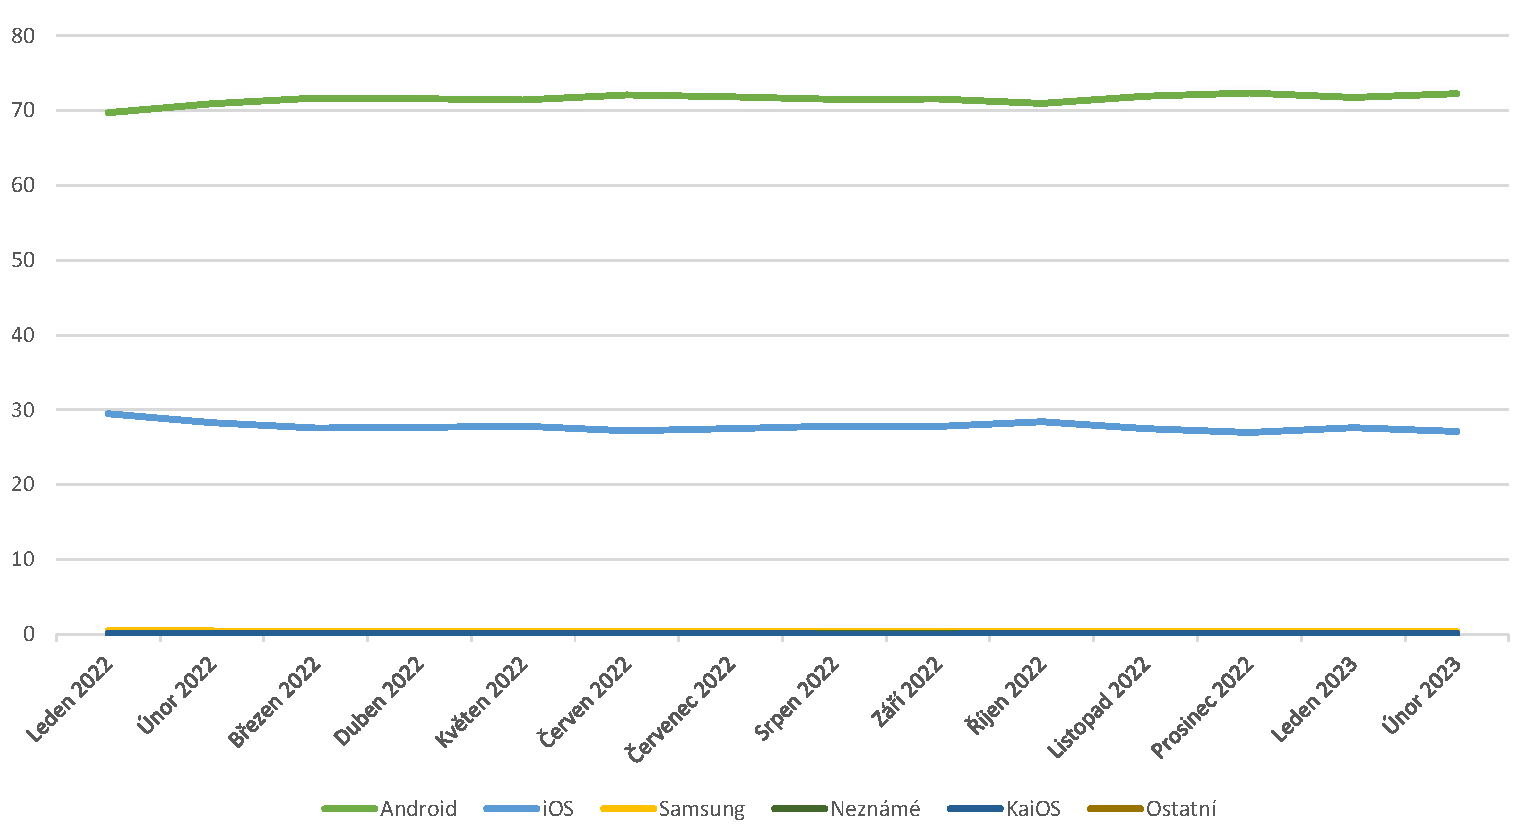
\includegraphics[width=1\textwidth]{Pictures/graf2.pdf}
	\caption{Podíl mobilních OS na trhu (v~\%) \cite{marketshare-mobile-os}}
	\label{fig:MarketshareMobileOS}
\end{figure}


\subsection{Webové aplikace}

Posledním možným řešením je webová aplikace. Webová aplikace je odlišná od desktopových a~mobilních tak, že je uložena na vzdáleném serveru a~uživatelé k~ní přistupují pomocí webového prohlížeče. Webové prohlížeče již bývají součástí operačních systémů, ať už desktopových nebo mobilních. Pro použití aplikace je potřeba mít přístup k~internetu, některé aplikace dokonce vyžadují neustálé připojení po celou dobu používání. 

Většina webových aplikací se skládá ze dvou hlavních částí - frontend a~backend. Frontend je část aplikace, která se zobrazuje uživateli ve webovém prohlížeči. Jedná se o~rozhraní, tlačítka, formuláře apod. Frontend je vytvářen jazyky jako HTML, CSS a~JavaScript. JavaScript se používá k~interakci s~uživatelem a~pro manipulaci obsahu stránky. Backend je taková část aplikace, která je umístěna na serveru a~zajišťuje různé výpočetní nebo datové operace. Důležitou vlastností backendu je, že dokáže zpracovávat požadavky frontendu a~dokáže pracovat s~databází.

Webové aplikace s~sebou nesou důležitou výhodu - jsou multiplatformní, což znamená, že tyto aplikace fungují na široké škále zařízení i~prohlížečů a~není tak potřeba vytvářet několik verzí pro různé systémy. Takové aplikace není třeba nijak lokálně instalovat, jejich aktualizace probíhají na straně serveru, kde jsou aplikace hostovány, takže uživatel vždy používá nejnovější verzi. V~dnešní době je nejvíce používaným webovým prohlížečem Google Chrome, který podporuje mnoho operačních systémů, např. Windows, macOS, Linux, Android nebo iOS. Jeho podíl na trhu přesahuje 65~\% všech webových prohlížečů \cite{marketshare-browser}. Díky rozsáhlé podpoře systémů tohoto prohlížeče lze zajistit kompatibilitu a~stejnou funkčnost na velkém množství zařízení.

Ideální aplikace pro naše využití by byla taková, která by byla snadno přístupná a~jednoduše použitelná na mnoha zařízeních. Po shrnutí různých typů aplikací jsem se rozhodl zvolit zrovna webovou. Webové aplikace mají dnes širokou škálu možností, dokážou stahovat data z~webových API, komunikovat se servery, tvořit grafy nebo i~vizualizovat mapu ČR. Tudíž by webová aplikace měla být schopna splnit to, co po ní v tomto případě vyžadujeme.

\section{Analýza požadavků vybraného řešení}

Když jsme zvolili webovou aplikaci jako vhodnou variantu, je potřeba zvážit a~zanalyzovat její požadavky, aby byla aplikace funkční a~pracovala správně. Pojďme si prvně ukázat jak obecně webové aplikace fungují:

\begin{enumerate}
    \item Uživatel přistoupí k~webové aplikaci prostřednictvím webového prohlížeče - frontend se stáhne z~webového serveru.
    \item Při interakci s~uživatelem (zmáčknutí tlačítka) může frontend zaslat požadavek na backend.
    \item Jakmile je požadavek předán backendu, provede požadovaný úkol - např. vypočte data nebo získá data z~databáze.
    \item Backend odešle zpět odpověď frontendu.
    \item Frontend zobrazí odpověď uživateli v~prohlížeči \cite{frontend-backend}.
\end{enumerate}

\subsection{Webový prohlížeč}

Podle prvního kroku je zcela zřejmé, že aby uživatel přistoupil k~aplikaci, musí použít webový prohlížeč. Budeme předpokládat, že uživatel bude přistupovat ze svého osobního počítače. Na této platformě patří mezi nejznámější prohlížeče Google Chrome a~jiné prohlížeče založené na projektu Chromium (Opera, Microsoft Edge), Mozilla Firefox nebo Safari. Vzhledem k~tomu, že tyto webové prohlížeče používají rozdílná jádra na zobrazování HTML, může výsledná aplikace vypadat na každém prohlížeči mírně jinak. Hlavní rozdíly lze spatřit u~ovládacích prvků (např. posuvníky nebo přepínače), protože každý prohlížeč používá svůj určitý design. Funkčnost aplikace by neměla být nijak ovlivněna.

\subsubsection*{Technologie použité ve webovém prohlížeči}

Každý moderní webový prohlížeč umí pracovat se třemi základními technologiemi, které jsou využité v~téměř každé webové aplikaci. Jedná se o~HTML, CSS a~JavaScript. Na tyto tři technologie se můžeme dívat tímto způsobem: HTML je konstrukce rodinného domu, CSS je dekorace interiéru a~exteriéru a~JavaScript je systém elektřiny, vody a~mnoha dalších funkčních prvků, díky kterým je dům obyvatelný \cite{what-is-html}.

HTML (\emph{Hyper Text Markup Language}) je značkovací jazyk pro vytváření webových stránek. Tento jazyk vyjadřuje jak je strukturovaný webový dokument a~jak by jej měl webový prohlížeč zobrazit. Struktura se skládá z~elementů vyznačené tagy. Elementy se skládají z~otevíracího tagu, obsahu a~uzavíracího tagu. Některé elementy ale mohou být prázdné, to znamená, že nemají uzavírací tag a~ani obsah, ale místo toho obsahují jediný tag, ve kterém mohou mít zdroj nebo odkaz na obsah, který chcete vložit na webovou stránku. Součástí elementu jsou i~atributy, které více definují chování nebo vzhled elementu \cite{google-scholar-html}. Na výsledné HTML stránce kódu \ref{src:HtmlListing} se nachází obrázek, nadpis a~jeden odstavec textu.

\begin{lstlisting}[style=htmlcssjs,label=src:HtmlListing,caption={Příklad HTML kódu}]
<!DOCTYPE html>
<html>
<body>
    <img src="https://www.w3.org/html/logo/badge/html5-badge-h-solo.png" alt="html_logo" >
    <h1> Toto je nadpis dokumentu </h1>
    <p> Zde je odstavec textu. </p>
</body>
</html>
\end{lstlisting}

CSS (\emph{Cascading Style Sheets}) je jazyk definující grafický vzhled HTML elementů ve webovém dokumentu. Pomocí CSS lze definovat vlastnosti (barvy, zarovnání, velikost písma atd.) pro každý element v~dokumentu. Díky tomuto jazyku můžeme styly definovat jednou pro celý dokument a~není třeba je opisovat při opakovaném použití v~dokumentu. Tyto styly se mohou uplatnit i~ve více dokumentech zároveň, např. v~celé webové aplikaci \cite{google-scholar-css}. Příklad CSS kódu, který styluje nadpisy, odstavce a~obrázky, se nachází v~kódu \ref{src:CssListing}. Porovnání webových stránek s~aplikovaným jednoduchým CSS a~bez stylu lze spatřit ve skupině obrázků \ref{fig:subfigures}.

JavaScript je objektově orientovaný programovací jazyk, který lze použít ve webových stránkách. Jedná se o~nezbytnou součást každé webové aplikace, díky které může webová stránka dynamicky měnit svůj obsah. JavaScript nám umožňuje aktualizovat obsah dokumentu, umístit interaktivní prvky, komunikovat se serverem nebo třeba i~vytvářet hry. Obecně díky JavaScriptu mohou získat webové dokumenty logiku a~dokážou být více responzivní a~interaktivní \cite{google-scholar-js}.


\begin{lstlisting}[style=htmlcssjs,label=src:CssListing,caption={Příklad CSS kódu}]
h1 {
    font-family: 'Brush Script MT', cursive;
    font-size: 40px;
    color: red;
    text-decoration: green solid underline;
}
p {
    font-family: 'Courier New', monospace;
    font-size: 20px;
    color: blue;
    background: aqua;
}
img {
    filter: grayscale(1);
}
\end{lstlisting}


\begin{figure}[h]
\centering
\subfloat[HTML kód \ref{src:HtmlListing} bez CSS stylování]{\label{fig:HTMLexampleWithoutCSS}{
\includegraphics[width=0.4\textwidth]{Pictures/html_kod.png}}}\hfill
\subfloat[HTML kód \ref{src:HtmlListing} s CSS kódem \ref{src:CssListing}]{\label{fig:HTMLexampleWithCSS}{
\includegraphics[width=0.4\textwidth]{Pictures/css_kod.png}}}
\caption{Jednoduchá ukázka porovnání CSS stylů}
\label{fig:subfigures}
\end{figure}


\subsection{Webový framework}
\label{sec:webframework}

Framework je softwarová struktura, která pomáhá při vývoji dalších softwarových projektů a~poskytuje podporu při programování. Tyto frameworky mohou obsahovat různé knihovny, podpůrné programy, návrhové vzory nebo ověřené postupy, zkrátka obsahují nástroje, které urychlují vývoj softwaru. Webový aplikační framework je speciální typ frameworku, který se zaměřuje na vývoj webových aplikací a~webových API. Frameworky často poskytují funkční základ, ke kterému můžeme přidat náš kód \cite{what-is-web-framework-geeks}. Použití nějakého webového aplikačního frameworku je nutné pro realizaci naší aplikace. Tyto frameworky dokážou zpracovávat HTTP požadavky, dokážou řídit a~spravovat databázi, mohou zlepšit zabezpečení a~tvořit výstupní data na základě požadavku uživatele \cite{what-is-web-framework-medium}. Příkladem tohoto typu frameworku mohou být např. Django, Ruby on Rails nebo ASP.NET.

\subsubsection*{Django}

Framework, který bude pro tuto práci využit, se jmenuje Django. Django je populární webový open-source framework napsaný v~programovacím jazyce Python. Je vyvinut na základě konceptu DRY (\emph{Don't Repeat Yourself}), který zdůrazňuje důležitost minimalizace duplicitního kódu. Django obsahuje mnoho vestavěných nástrojů jako jsou například správa uživatelů, autentizace a~správa databází. Tento framework je založen na architektuře MTV (\emph{Model-Template-View}), která je hodně podobná architektuře MVC (\emph{Model-View-Controller}). To poskytuje oddělení logiky, uživatelského rozhraní a~datového modelu \cite{django-dry,django-online-dokumentace}. 

Funkce v Djangu, které zpracovávají webové požadavky a~vrací odpovědi, se nazývají zobrazení (\emph{views}) a~jsou uloženy ve \emph{views.py}. Aby Django věděl jakou z~těchto funkcí má spustit, používá URL mapovač v~\emph{urls.py}, který přesměrovává požadavky danému zobrazení podle URL požadavku. Navíc může tento mapovač předat data do zobrazení, která byla obsažena v~URL adrese (např. data formulářů). Django také umí pracovat s~modely (\emph{models.py}). Každý tento model je třída, která se mapuje do jedné databázové tabulky. Na základě těchto modelů Django automaticky vygeneruje API, které umožňuje spravovat (přidávat, upravovat, odstraňovat) záznamy v~databázi. K~zobrazování a~generování stránek a~jejich obsahu využívá tento framework šablony (\emph{templates}). Podle těchto šablon se generují webové stránky a~mohou se naplnit daty z~modelů nebo jiných zdrojů \cite{what-is-django}. Zjednodušený postup zpracování HTTP požadavku Djangem lze vidět na obrázku \ref{fig:DjangoDiagram}.

\begin{figure}
	\centering
	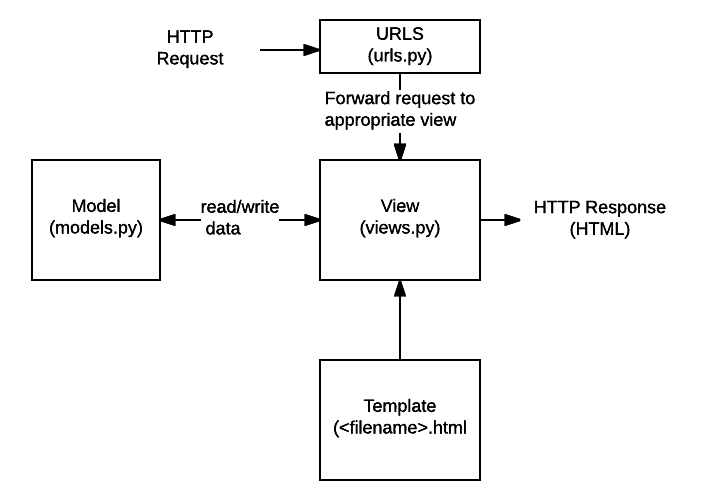
\includegraphics[]{Pictures/django-diagram.png}
	\caption{Postup zpracování HTTP požadavku v Djangu \cite{what-is-django}}
	\label{fig:DjangoDiagram}
\end{figure}

\subsection{Databáze}
\label{sec:DatabaseTheory}

Tato aplikace pracuje s~daty onemocnění covid-19, přístup k~nim nám umožňuje API portálu Onemocnění aktuálně. Vzhledem k~tomu, že je toto API veřejné a~je k~němu teoreticky neomezený přístup, nemusí nám toto API vždy rychle odpovědět. Proto by bylo vhodné mít data uložena lokálně v~backendu. To nám umožní si data libovolně předzpracovat a~díky tomu můžeme urychlit aplikaci. Nejlepší metoda pro ukládání dat by byla pravděpodobně použití databáze. Databáze je z~hlediska IT organizovaná sada strukturovaných informací nebo dat, které jsou uloženy v~elektronické podobě v~počítačovém systému. Tyto databáze ve většině případů používají strukturovaný dotazovací jazyk SQL pro manipulaci samotné databáze a~dat. Databáze obvykle vyžadují správu pomocí systému řízení báze dat (DBMS) \cite{what-is-database-oracle}.

Databázový systém, který je použitý pro tuto aplikaci, se nazývá SQLite. SQLite je relační databázový systém, který se používá pro ukládání dat v~souborech. Jedná se o~open-source software, který je zdarma dostupný pro použití v~komerčních i~nekomerčních projektech. Jeho důležitou vlastností je malá velikost a~nenáročnost. To znamená, že SQLite soubory mohou být velmi malé, často v~rámci jednotek MB, i~přesto, že mohou obsahovat velké množství dat. SQLite podporuje většinu standardních SQL příkazů, což znamená, že se s~ním lze snadno pracovat, pokud máte zkušenosti s~jinými relačními databázovými systémy. SQLite také umožňuje vytváření indexů pro rychlejší vyhledávání dat a~podporuje transakce pro zajištění konzistence dat \cite{what-is-sqlite}.

Jak bylo zmíněno, SQLite pracuje s~jednoduchými databázovými soubory. Pro práci s~těmito soubory bylo vytvořeno mnoho softwaru, mezi takové programy patří např. DB Browser for SQLite. Jedná se o~kvalitní open-source vizuální nástroj pro vytváření, navrhování a~úpravy databázových souborů kompatibilních s~SQLite. Tento program bude použit pro vytvoření databáze a~práci s~ní. Ukázka tohoto programu je na obrázku \ref{fig:SQliteScreenshot}.

Díky své jednoduchosti a~malé velikosti je SQLite ideální pro toto použití, v~tomto případě není třeba používat složitější relační databázové systémy jako např. MySQL.

\begin{figure}
	\centering
	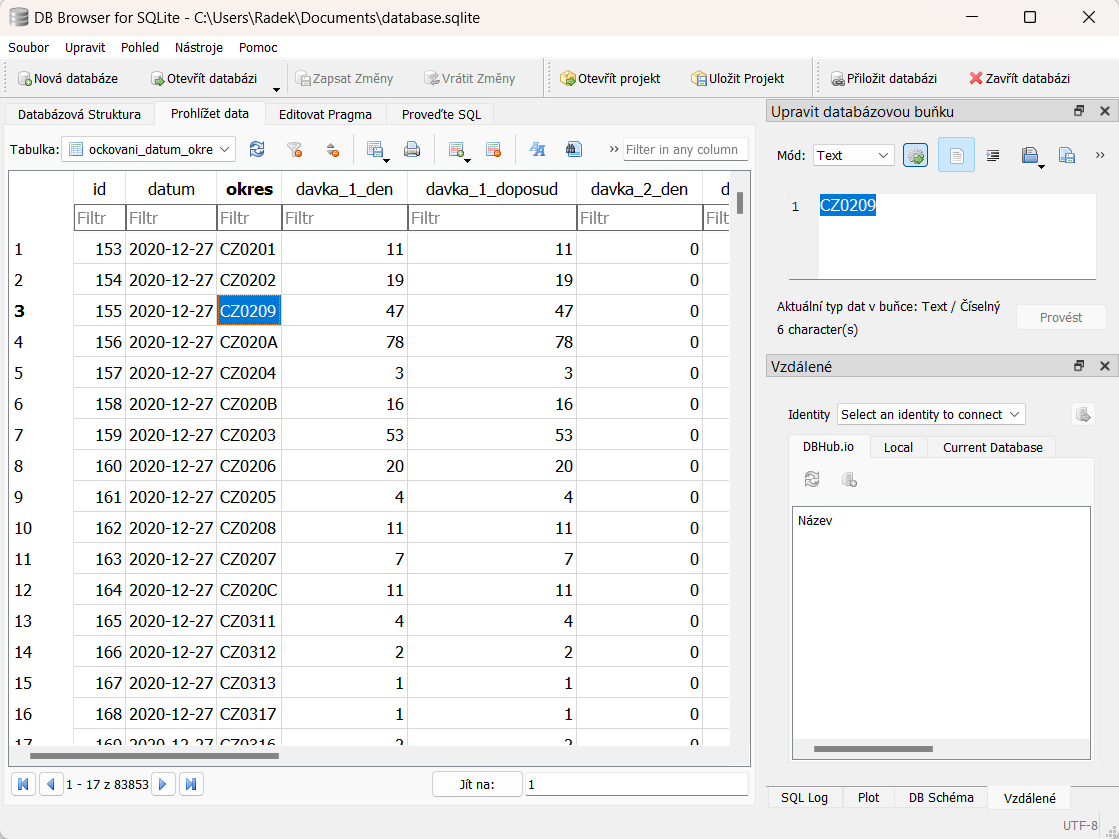
\includegraphics[width=0.8\textwidth]{Pictures/screen_sqlite.png}
	\caption{Program DB Browser for SQLite s~otevřeným databázovým souborem \cite{dbbrowser}}
	\label{fig:SQliteScreenshot}
\end{figure}

\subsection{Způsob vizualizace okresů}
\label{sec:GeoJSON}

Existuje několik způsobů jak vizualizovat územní celky státu na mapě. Byla zvolena možnost vyobrazení pomocí GeoJSONu neboť je tento formát používán v~knihovně, která bude využita pro vytvoření interaktivní mapy.

GeoJSON je formát pro kódování různých geografických datových struktur pomocí JSONu. To umožňuje zakódovat různé geometrické útvary - body, linie, mnohoúhelníky a~další útvary a~dokáže k~nim přidat různé další vlastnosti. Tyto zakódované útvary jsou tzv. GeoJSON objekty. Sady těchto objektů jsou obsaženy v~nadúrovňových objektech \lstinline{FeatureCollection} nebo \lstinline{GeometeryCollection} \cite{google-scholar-geojson}. Každý útvar je definován svým typem a~souřadnicemi na mapě. Ke každému útvaru lze také připsat dodatečné informace, třeba o~jaké místo se jedná.

Pro tvorbu GeoJSON souborů existuje mnoho nástrojů, ve velké většině z~nich se jedná o~webové aplikace. Jedním z~nich je GeoJSON.io \cite{geojson.io}. Tento online nástroj umožňuje nejen vytvářet GeoJSON soubory, ale také dokáže pracovat s~jinými typy souborů a~vyobrazovat je na mapě. Umí pracovat s~formáty jako GPX, CSV, KML nebo samotným GeoJSON \cite{geojson.io}.

Aplikace obsahuje interaktivní mapu s~nástroji kreslení geometrických útvarů. Po dokončení útvaru vám aplikace na pravé straně stránky převede daný útvar do GeoJSONu. Poté stačí kód zkopírovat a~data jsou hotova. Na obrázku \ref{fig:GeoJson.ioScreen} lze vidět aplikaci společně s~vytvořeným kódem pro lokaci Katedrály sv. Víta v~Praze.

\begin{figure}[h]
	\centering
	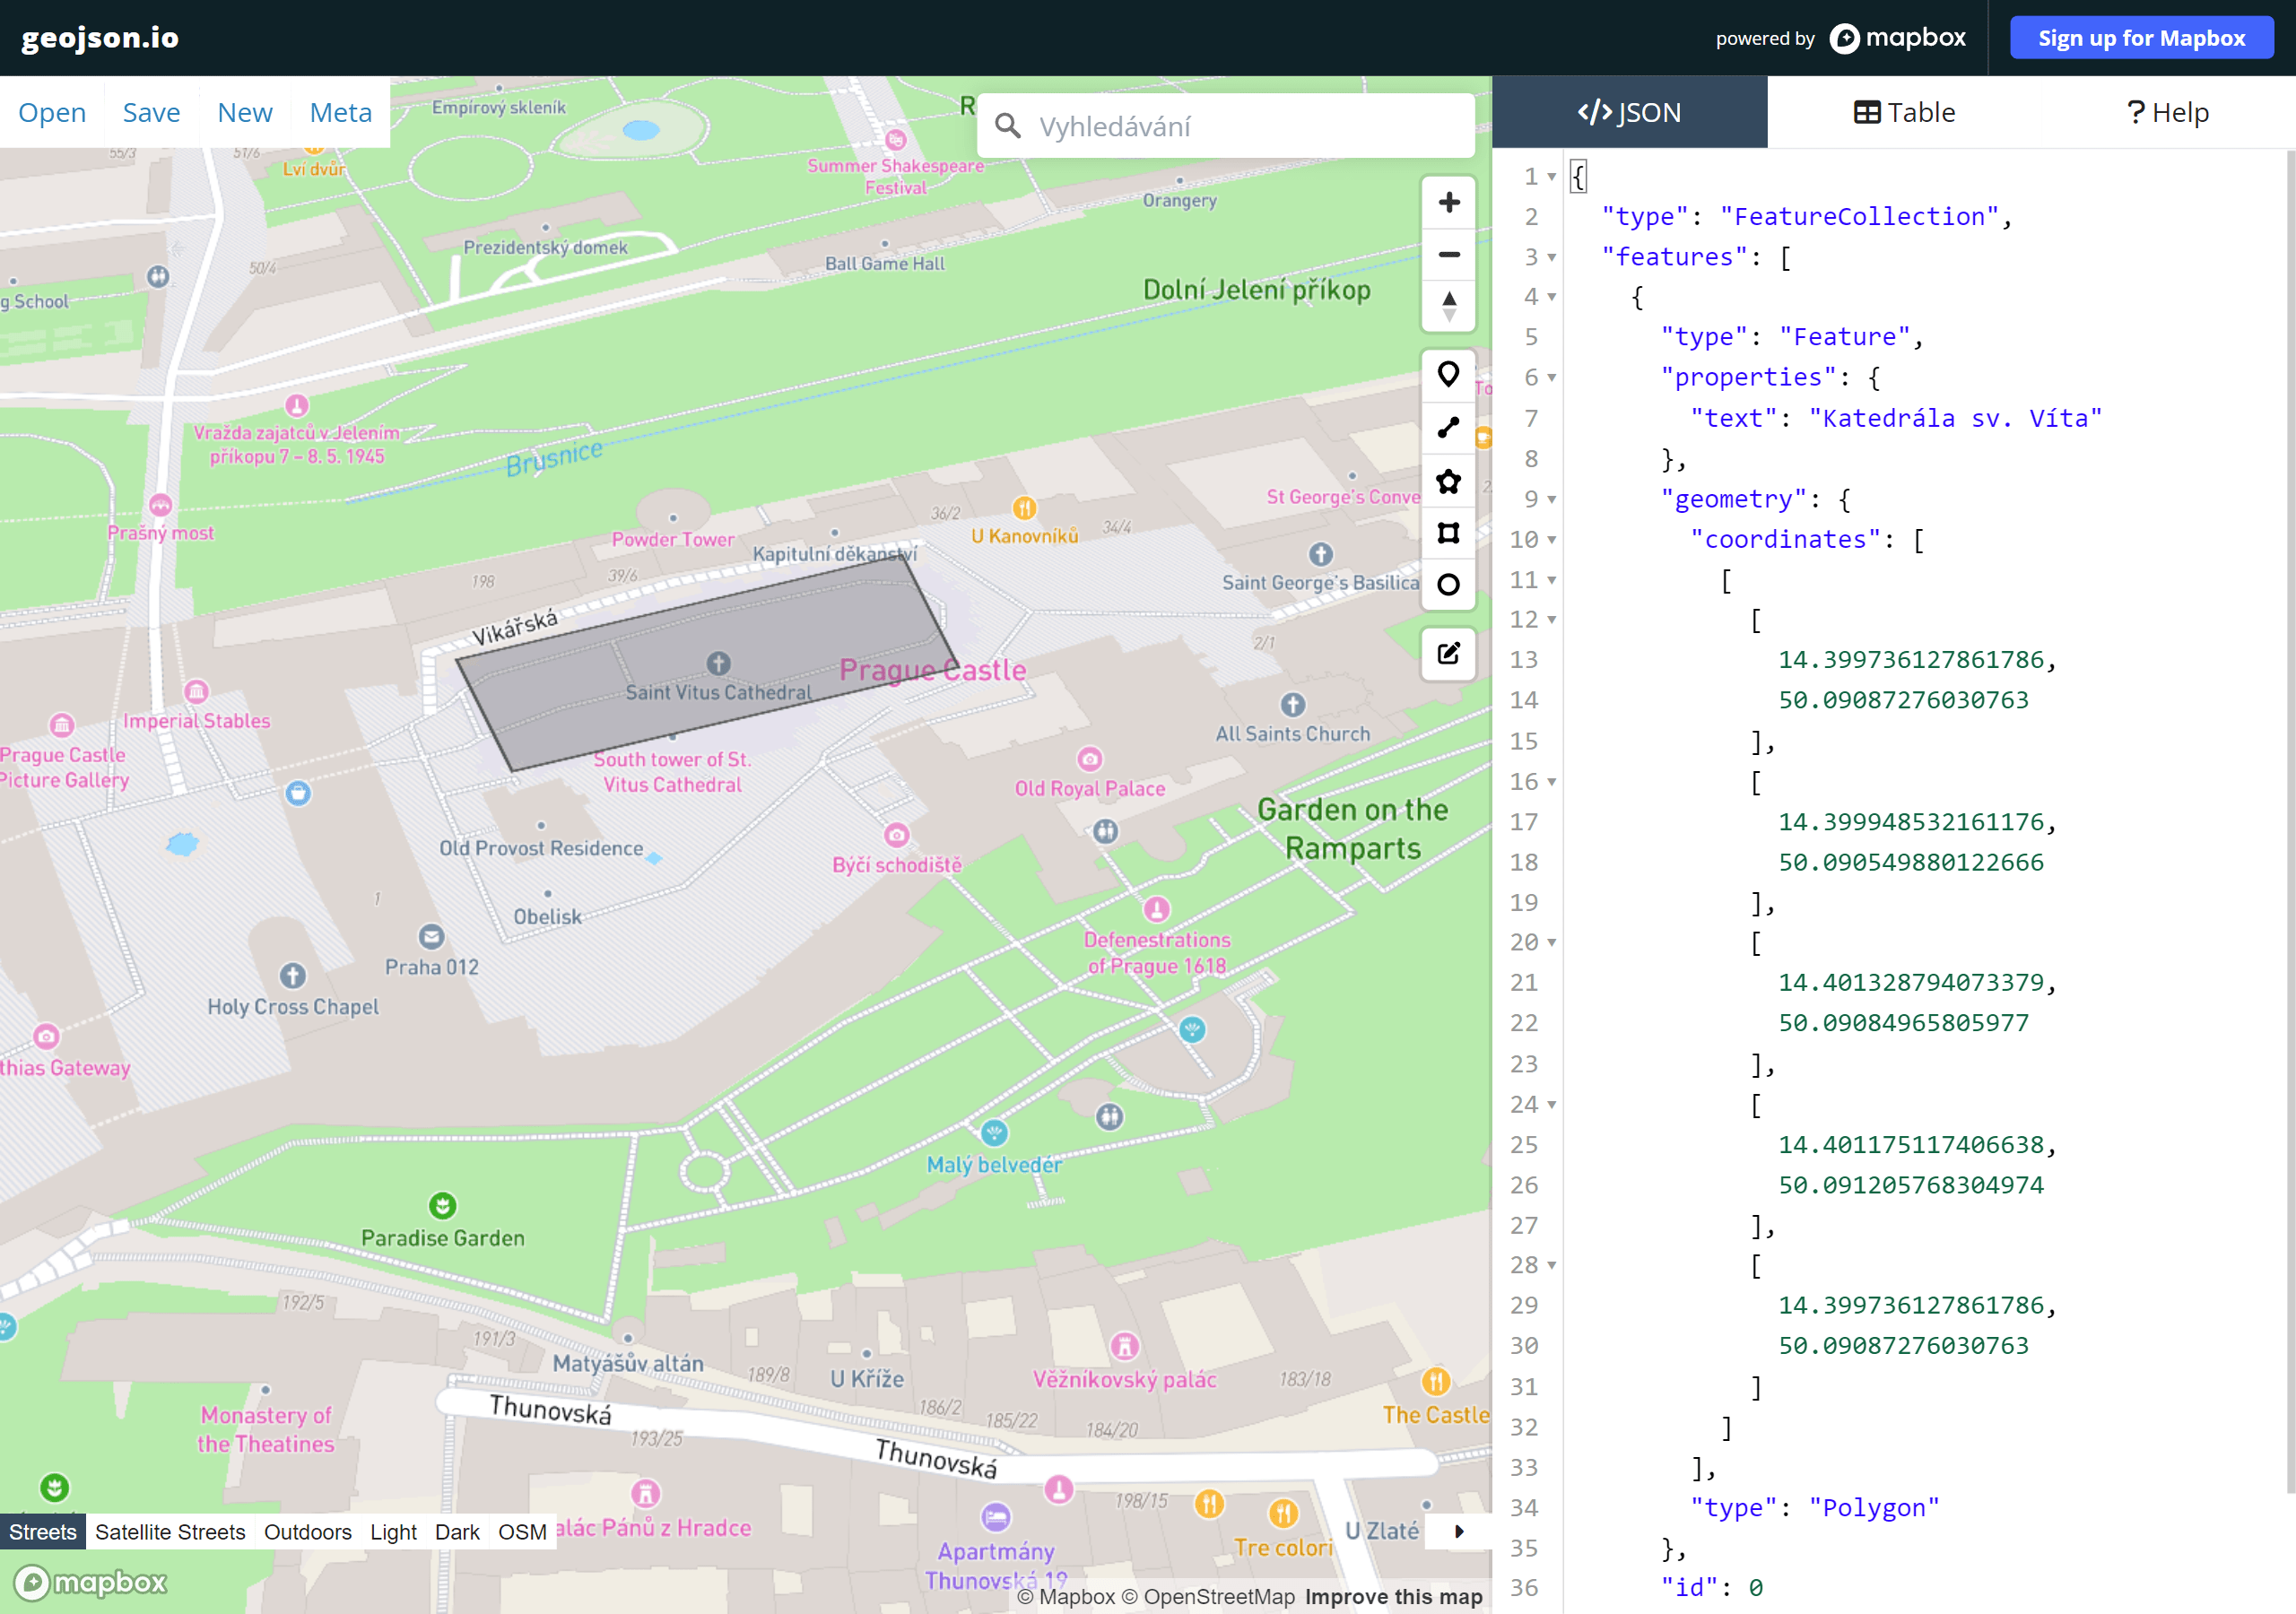
\includegraphics[width=1\textwidth]{Pictures/geojson_screen.png}
	\caption{Práce s~webovou aplikací geojson.io \cite{geojson.io}}
	\label{fig:GeoJson.ioScreen}
\end{figure}
\chapter{Popis řešení}

\section{Shrnutí vybraného řešení}

Po zkoumání různých řešení bylo rozhodnuto, že nejvhodnějším řešením bude webová aplikace. Hlavním prvkem této aplikace je webový aplikační framework Django, který bude provozován na serverové straně. Celý framework je napsán v~programovacím jazyce Python, což znamená, že veškerá logika na straně serveru bude psána ve stejném jazyce. Pojďme se nyní podívat co bude hlavními úkoly serverové části (backendu):

\begin{itemize}
    \item stahovat nová data z~API Onemocnění aktuálně,
    \item ukládat stažená data do lokální databáze,
    \item vytvořit cache, která bude obsahovat rychle přístupná covidová data,
    \item odpovídat frontendu na jeho HTTP požadavky a~zasílat zpět vyžádaná data z~cache.
\end{itemize}

Strana klienta obsahuje uživatelské prostředí, které bude realizováno díky HTML a~CSS. Logická část aplikace poběží na pozadí webového prohlížeče, k~tomu dojde prostřednictvím JavaScript kódu, jež se automaticky spustí při načtení aplikace. Nyní si shrňme, co by měla zvládnout strana klienta (frontend):

\begin{itemize}
    \item požádat backend o~data,
    \item získaná data případně zpracovat a~poté zvizualizovat,
    \item interagovat s~uživatelem a~odpovídat na jeho požadavky (např. změna časového okna, přizpůsobení vizualizace atd.).
\end{itemize}

Kromě vysvětlení serverové a~klientské části aplikace bude také popsáno vytvoření interaktivní mapy a~její přizpůsobení, instalace a~nastavení frameworku Django, práce s~databází a~další. Zjednodušený use case diagram, který znázorňuje případy užití těchto dvou částí aplikace, je k~dispozici v~příloze \ref{fig:Diagram3}.

\subsection{Popis použití aplikace uživatelem}

Hlavní způsob, jak lze tuto webovou aplikaci použít, je přistoupit na webovou stránku aplikace. Jakmile uživatel na tuto stránku přistoupí, server automaticky zkontroluje, zda má aktuální data. Pokud jsou data aktuální, odešle odpověď uživateli ve formě HTML stránky, která obsahuje uživatelské prostředí a~interaktivní mapu. V~tento moment získává uživatel přístup k~vizualizaci covidových dat. Aby mohl uživatel vizualizaci dat ovládat, musí nejprve zvolit dataset a~časově okno. Po zvolení těchto možností zbývá uživateli stisknout tlačítko na stažení dat. Po stisknutí tlačítka dojde k~odeslání žádosti o~data na nově vytvořené API. API může buď vrátit chybový kód v~případě chyby nebo může vrátit data ve formě JSONu. Tato data aplikace na straně uživatele automaticky zpracuje a~následně spustí vizualizaci. Uživatel si poté může vizualizaci libovolně přizpůsobit nebo případně může stáhnout data pro jiné časově okno.

\section{Instalace a~nastavení Djanga}

Celý kód k~instalaci Djanga a potřebných balíčků je k~dispozici v příloze \ref{src:DjangoInstall}. V~této příloze se nachází i~příklad vytvoření projektu a~aplikace v~Djangu. Je nutné podotknout, že k~vykonání určitých částí kódu jsou potřeba zvýšená práva uživatele

\subsection{Python}

Django je webový framework založený na programovacím jazyce Python. Python je vysokoúrovňový interpretovaný objektově-orientovaný programovací jazyk, který nevyžaduje kompilaci nebo linkování. Díky tomu se s~tímto jazykem může vyvíjet software rychleji oproti jiným jazykům jako například C++. Je relativně jednoduchý k~použití a~je dostupný na mnoha operačních systémech. Je také známý pro svou snadnou čitelnost a~zápis \cite{google-scholar-python}. Pro zprovoznění Djanga je nutné mít v~systému nainstalovaný Python. Na webových stránkach Pythonu \cite{python-download} je k~dispozici instalátor pro systémy Windows nebo macOS. V~případě systému Linux je možné nainstalovat Python přes terminál, často ale bývá již předinstalovaný. Zjištění aktuální verze Pythonu společně s~instalací lze vidět na kódu v příloze \ref{src:DjangoInstall}.

\subsection{Pip}

Společně s~Pythonem je nutný pro instalaci Djanga pip. Jedná se o~instalační program balíčků pro Python, který dokáže instalovat balíčky z~Python Package Index a~jiných zdrojů \cite{pip-python}. Pip použijeme pro instalaci Djanga. V~příloze \ref{src:DjangoInstall} se prvně kontroluje, zda je pip nainstalovaný, a~poté se instaluje. Jakmile je nainstalovaný pip, můžeme jej využít k~instalaci balíčků pro Python.

\subsection{Virtuální prostředí}

Při instalaci balíčků přes pip se doporučuje používat oddělená virtuální prostředí. Tato prostředí jsou praktičtější, protože umožňují instalovat balíčky bez oprávnění správce a~budou nainstalovány pouze v~daném odděleném prostředí, nikoli v~celém systému. Samotnému prostředí můžeme přiřadit i~určitou verzi Pythonu, kterou si zvolíme \cite{venv-dokumentace}. Příklad vytvoření virtuálního prostředí je možné spatřit v~příloze \ref{src:DjangoInstall}.

\subsection{Instalace Djanga a~ostatních balíčků}

Jakmile je vše připraveno pro instalaci frameworku Django, nainstalujeme jej přes instalátor balíčků pip. Instalaci Djanga lze spatřit v kódu \ref{src:DjangoInstall}, kde jej nainstalujeme do vytvořeného virtuálního prostředí. Před instalací můžeme zkontrolovat, zda již náhodou není Django nainstalován. Mimo Django bude ještě potřeba knihovna APScheduler (\emph{Advanced Python Scheduler}), díky které je v~aplikaci zprovozněna automatická aktualizace covidových dat.

\subsection{Vytvoření projektu v~Djangu}

Abychom mohli vyvíjet webovou aplikaci, je potřeba vytvořit nový projekt v~Djangu. Projekt v~Djangu můžeme chápat jako prostředí, ve kterém budeme vyvíjet vlastní webovou aplikaci \cite{django-online-dokumentace}. Ve vytvořeném projektu si následovně vytvoříme novou aplikaci s názvem \emph{covid}. Vytvoří se nová aplikace se základní konfigurací, která je funkční již při vytvoření. Opět je vytvoření projektu a aplikace dostupné v příloze \ref{src:DjangoInstall}. 

\subsection{Nastavení projektu}

\subsubsection*{Nastavení šablon a~otestování zobrazení}

Po vytvoření aplikace dojde k~vytvoření adresáře, který obsahuje několik konfiguračních souborů. Nejdůležitější soubory v~adresáři aplikace jsou \emph{urls.py}, \emph{views.py} a~\emph{models.py}. Pro otestování si vyzkoušíme vrátit jednoduchou webovou stránku z~šablony. Nejprve je nutné v~projektu specifikovat cestu k~šablonám. Vytvoříme si nový adresář ve složce s~projektem a~nastavíme projekt, aby používal tento adresář k~procházení šablon. Nastavení šablon lze vidět v~kódu \ref{src:DjangoPythonSetupTemplates}, kde se specifikuje vytvořený adresář \emph{templates} v~soubouru \emph{settings.py}.

\begin{lstlisting}[language=Python,label=src:DjangoPythonSetupTemplates,caption={Nastavení šablon v Django projektu \cite{django-online-dokumentace}}]
# Soubor settings.py
TEMPLATES = [
    {
        'BACKEND': 'django.template.backends.django.DjangoTemplates',
        # 'DIRS' obsahuje seznam názvů adresářů s šablonami
        'DIRS': ['templates'],
        'APP_DIRS': True,
        'OPTIONS': {
            # ... nastavení zde ...
        },
    },
]
\end{lstlisting}

Jako příklad využijeme HTML kód \ref{src:HtmlListing}, který si uložíme do adresáře s~šablonami s~názvem \emph{index.html}. V~souboru \emph{views.py} v~adresáři s~aplikací si vytvoříme nové zobrazení s~názvem \emph{index}. Tomuto zobrazení nastavíme, že má jako výsledek vrátit danou šablonu. Výsledné zobrazení lze spatřit v~kódu \ref{src:DjangoPythonDefaultView}.

\begin{lstlisting}[language=Python,label=src:DjangoPythonDefaultView,caption={Přikladné zobrazení v Djangu s~využitím šablony}]
from django.shortcuts import render

def index(request):
    return render(request, 'index.html')
\end{lstlisting}

Na závěr je potřeba namapovat dané URL, aby při zaslání požadavku na toto URL zaslal server zpět výsledek vytvořeného zobrazení. Nejprve specifikujeme v~souboru \emph{urls.py} v~adresáři projektu, aby projekt namapoval všechny URL z~naší vytvořené aplikace. Následně v~adresáři s~aplikací v~souboru \emph{urls.py} namapujeme vytvořené zobrazení s~danou URL. Výsledné soubory lze vidět v~kódu \ref{src:DjangoPythonURLMapping}.

\begin{lstlisting}[language=Python,label=src:DjangoPythonURLMapping,caption={Namapování URL v projektu a aplikaci Djanga \cite{django-online-dokumentace}}]
# Nově upravený soubor urls.py v adresáři projektu
from django.contrib import admin
from django.urls import include, path
import covid.views

urlpatterns = [
    path('covid/', include('covid.urls'))
]

# Nově upravený soubor urls.py v adresáři aplikace
from django.urls import path
import covid.views

urlpatterns = [
    path('index/', covid.views.index, name='index')
]
\end{lstlisting}

Nyní aplikace vrací kód \ref{src:HtmlListing} při přistoupení na adresu \url{https://127.0.0.1:8000/covid/index}. Po celou dobu práce s~Djangem se bude používat lokální testovací server, který umožňuje snadné testování aplikace.

Při vytváření aplikace bude projekt nastaven v~tzv. vývojovém režimu. Při tomto režimu má projekt nastavený klíč \texttt{DEBUG} v~souboru \emph{settings.py} na \texttt{True}. To umožní snazší vývoj aplikace, neboť bude aplikace detailně zobrazovat veškeré chyby během používání ve webovém prohlížeči společně s~jinými dodatečnými informacemi. Tento režim by měl být vypnut při finálním nasazení na server. Pro testování aplikace je aplikaci možno spustit lokálně pomocí příkazu \lstinline{python3 manage.py runserver} v~adresáři s~projektem a~je možné k~ni přistoupit na adrese \url{https://127.0.0.1:8000}.

\subsubsection*{Statické soubory}

Součástí každé webové aplikace jsou statické soubory. Může se jednat o~různé obrázky, kaskádové styly nebo i~JavaScript soubory. Django ve svém defaultním nastavení neposkytuje statické soubory, bude třeba je zapnout. Pro začátek je nutné Djangu specifikovat novou aplikaci, kterou má použít, jedná se o~aplikaci \lstinline{django.contrib.staticfiles}, která spravuje statické soubory. Následně stačí nastavit dva klíče \texttt{STATIC\_URL} a~\texttt{STATICFILES\_DIRS} tak, aby ukazovaly na adresář se statickými soubory. Pro jejich správné nastavení bude možná potřeba znát kořenový adresář Django projektu. Získání tohoto adresáře (\texttt{BASE\_DIR}) můžeme vidět v~kódu \ref{src:DjangoStaticFiles}, který obsahuje změny konfigurace projektu. Po správném nastavení se cesta ke statickým souborům definuje v~šablonách pomocí speciální značky \lstinline[language=bash]||, v šabloně se také musí na začátku dokumentu nacházet kód, který umožní statické soubory používat - \lstinline[language=bash]||.

\begin{lstlisting}[language=Python,label=src:DjangoStaticFiles,caption={Nastavení statických souborů v Djangu \cite{django-static}}]
from pathlib import Path
import os

BASE_DIR = Path(__file__).resolve().parent.parent

INSTALLED_APPS = [
    # ... aplikace ... #
    'django.contrib.staticfiles'
]

STATIC_URL = 'covid/static/'

STATICFILES_DIRS = ( os.path.join(BASE_DIR, 'covid/static'))

\end{lstlisting}

\subsubsection*{X-Frame-Options}

Mezi další nastavení, která jsou v~případě této aplikace nutná, patří nastavení \emph{X-Frame-Options}. Jedná se o~bezpečnostní hlavičku, která slouží k~ochraně webových stránek před útoky typu \enquote{clickjacking}. Clickjacking je typ útoku na webovou stránku, při kterém útočník zavádí uživatele ke kliknutí na odkaz nebo tlačítko na stránce bez jeho vědomí. Zdrojem tohoto útoku často bývá využití tagu \emph{iframe}, který je neprůhledný a~ve kterém se nachází stránka útočníka \cite{google-scholar-clickjacking}. Hlavička \emph{X-Frame-Options} říká prohlížeči, zda má nebo nemá povolit načtení webové stránky v~rámci \emph{iframe} \cite{mozilla-xframe}. V~našem případě je potřeba hodnota \texttt{SAMEORIGIN}, to znamená, že by měl prohlížeč umožnit načtení webové stránky v~rámci \emph{iframe} pouze v~případě, že je URL v~\emph{iframe} na stejné doméně jako webová stránka. Toto je nutné, abychom mohli zobrazit interaktivní mapu zvlášť v~\emph{iframe} mimo hlavní dokument. Pro nastavení této hlavičky je potřeba přidat middleware \lstinline{django.middleware.clickjacking.XFrameOptionsMiddleware} do nastavení projektu. Změněnou konfigurace lze vidět v~kódu \ref{src:DjangoXFrame}.

\begin{lstlisting}[language=Python,label=src:DjangoXFrame,caption={Nastavení X-Frame-Options v Djangu}]
MIDDLEWARE = [
    # ... náš middleware ...
    'django.middleware.clickjacking.XFrameOptionsMiddleware',
]

X_FRAME_OPTIONS = 'SAMEORIGIN'

\end{lstlisting}

\subsubsection*{Provedení akcí při startu frameworku}

Jakmile dojde ke spuštení frameworku Django, provede se několik důležitých akcí. Mezi hlavní patří načtení cache, která se později využívá v~programu. Dodatečně také dojde k~pokusu o~aktualizaci covidových dat a~spuštení úlohy, která se automaticky každou hodinu pokouší aktualizovat data. Aby bylo možné spustit kód při spuštění aplikace, je nutné upravit konfiguraci aplikace v~Djangu. Konfigurace aplikace se nachází v~adresáři aplikace v~souboru \emph{apps.py}. V~tomto souboru se nachází třída, která odpovídá názvu aplikace s~příponou \enquote{Config}. Do této třídy se vloží nová metoda \lstinline{ready}, ve které se bude nacházet kód, který se má spouštět při startu aplikace. Výslednou třídu lze vidět v~následujícím kódu \ref{src:DjangoStartup}. Na závěr je nutné přidat tuto upravenou konfiguraci do listu \texttt{INSTALLED\_APPS} v~souboru \emph{settings.py}. V~našem případě se jedná o~přidání \lstinline{covid.apps.CovidConfig}.

\begin{lstlisting}[language=Python,label=src:DjangoStartup,caption={Změna konfigurace aplikace v Djangu}]
from django.apps import AppConfig

class CovidConfig(AppConfig):
    default_auto_field = 'django.db.models.BigAutoField'
    name = 'covid'

    def ready(self):
        # Načtení cache
        # Aktualizace covidových dat
        # Spuštění automatické úlohy na aktualizaci dat
\end{lstlisting}

\subsubsection*{Automatická aktualizace covidových dat}

Aplikace je připravena na takovou situaci, kdy k~ní po dlouhou dobu nepřistoupí žádný uživatel. Původně by to způsobilo neaktuálnost dat, protože si aplikace aktualizuje data až při přístupu na její webovou stránku uživatelem. Tuto situaci řeší úloha, která se automaticky spouští každou hodinu. Toto je realizováno knihovnou APScheduler, která umožňuje plánovat úlohy v~jazyce Python. Náplní této úlohy je kontrola aktuálnosti dat, pokud data nejsou aktuální, stáhnou se nová data a~aktualizuje se cache. Aby bylo možné spouštět nějakou úlohu po daný interval, byla vytvořena nová funkce, která obsahuje kód, jež nastavuje danou úlohu. Jedná se o~funkci \lstinline{start_auto_updater} v~souboru \emph{tasks.py}. Ukázku spuštění úlohy lze spatřit v~kódu \ref{src:DjangoTask}.  

\begin{lstlisting}[language=Python,label=src:DjangoTask,caption={Nastavení plánované úlohy pomocí apscheduler}]
from apscheduler.schedulers.background import BackgroundScheduler
from exec.updater import *

def start_auto_updater():
    scheduler = BackgroundScheduler()
    scheduler.add_job(Updater.update_data, 'interval', hours=1)
    scheduler.start()
\end{lstlisting}

\section{Interaktivní mapa}

\subsection{Vytvoření GeoJSONu}

Princip a~fungování GeoJSONu byly vysvěleny v~kapitole \ref{sec:GeoJSON}. Pomocí online nástroje geojson.io \cite{geojson.io} byl vytvořen GeoJSON soubor, který obsahuje informace o~rozdělení České republiky na okresy. Vzhledem k~náročnosti vytváření takových map nemusí být mapa přesně rozdělena. Výsledný výstup GeoJSONu lze vidět na obrázku \ref{fig:GeoJSONczechia}.

\begin{figure}[h]
	\centering
	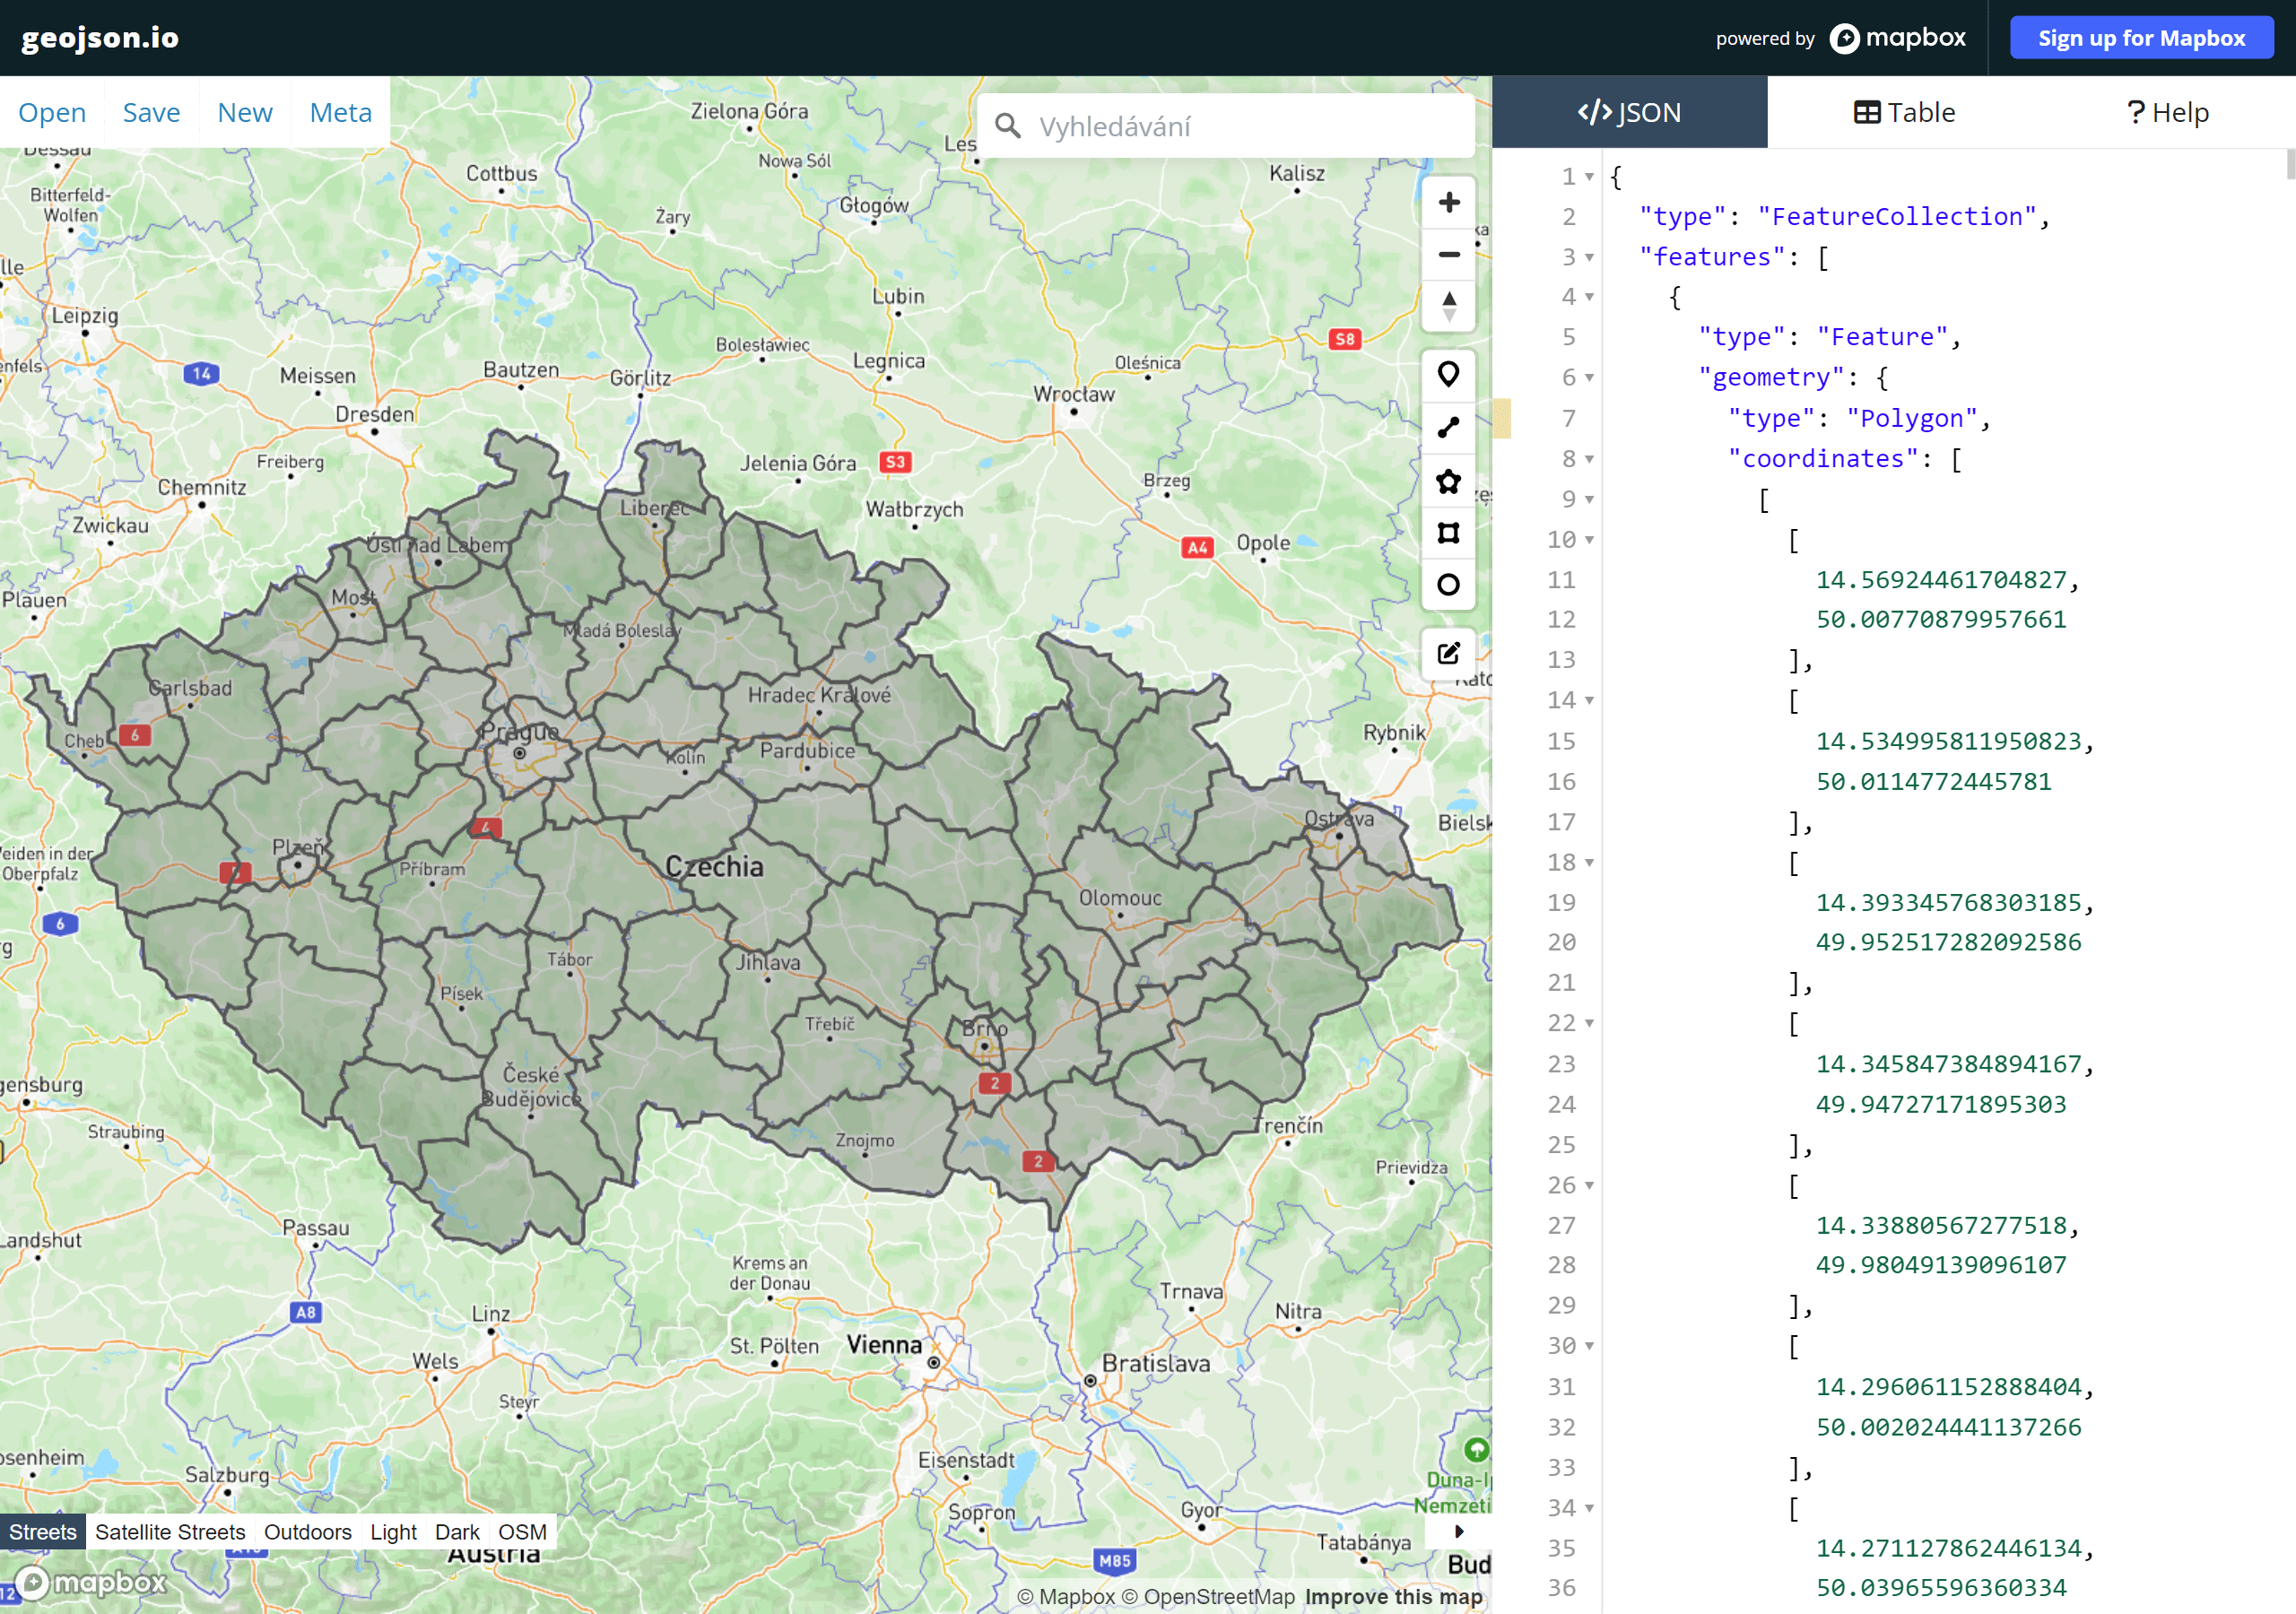
\includegraphics[width=0.87\textwidth]{Pictures/geojson_czech.png}
	\caption{Vytvoření GeoJSONu v~nástroji geojson.io \cite{geojson.io}}
	\label{fig:GeoJSONczechia}
\end{figure}

\subsection{Vytvoření mapy}
\label{map_creation}

Jedna z~mnoha knihoven, které umožňují vytváření interaktivních map z~GeoJSONu, je Folium. Folium je knihovna pro Python, která se používá pro vytváření interaktivních Leaflet map. Leaflet je open-source JavaScriptová knihovna zaměřená na tvoření interaktivních map s~možnostmi jako přibližování, vrstvování nebo zobrazování bodů na mapě. Je vysoce přizpůsobitelná a~pracuje s~poskytovateli map jako OpenStreetMap, Mapbox a~jinými \cite{leafletjs-dokumentace}. Folium používá tuto knihovnu, aby vytvořil konečnou interaktivní mapu ve formátu HTML, kterou lze otevřít ve webovém prohlížeči. Jednou ze schopností Folia je, že dokáže pracovat s~GeoJSONem a~že dokáže zobrazit jeho obsah na výsledné mapě s~interaktivními prvky (např. po kliknutí na okres se zobrazí informace).

Celý proces vytvoření mapy lze spatřit v~příloze \ref{src:CreateMapFolium}. Prvně dochází k~vytvoření prázdného mapového objektu. Následně je načtený GeoJSON s~okresy České republiky ze souboru a~poté je uložen do proměnné. Poté se vytvoří nová mapová vrstva s~nastaveným GeoJSONem a~přidá se do nově vytvořeného mapového objektu. Dále následuje nastylování objektů GeoJSONu a~styl vyskakovacích oken společně s~\enquote{hoverem}. Na závěr přidáme tato nastavení do mapového objektu, přidáme mapový objekt do seznamu vrstev celkové mapy a~uložíme vytvořenou mapu do HTML souboru.

Výstupem je HTML interaktivní mapa, která bude použita ve výsledné aplikaci. Některé prvky mapy se budou měnit za chodu aplikace, např. zvýraznění vybraného okresu, barvy nebo průhlednost okresů.

\section{Popis důležitých komponent a~částí backendu}

V~této podkapitole budou popsány veškeré důležité funkce a~části backendu. Základem backendu je framework Django, který dokáže přijímat požadavky z~frontendu.

\subsection{Databáze}

V~kapitole \ref{sec:DatabaseTheory} bylo zmíněno, že k~realizaci ukládání dat z~API Onemocnění aktuálně bude využita SQLite databáze. Pro ukládání dat o~koronaviru bude využita externí SQLite databáze mimo framework, která bude obsahovat pouze informace o~koronaviru, nikoli i~informace o~Django projektu, které jsou obsaženy v~původní Django databázi.

\subsubsection*{Vytvoření databáze}

K~vytvoření databáze bude použit program DB Browser for SQLite. Ukázku programu lze vidět na obrázku \ref{fig:SQliteScreenshot}. V~kapitole \ref{sec:onemocneni-aktualne} byly zmíněny datasety, ze kterých bude aplikace čerpat data. Aplikace bude zobrazovat celkem čtyři kategorie dat - infekce, úmrtí, očkování a~PCR testování. V~databázi se bude také uchovávat číselník ORP, který slouží k~přiřazení ORP do okresu. Podle těchto kategorií bude vytvořena databáze s~následujícími tabulkami:

\begin{itemize}
    \item \emph{covid\_infections},
    \item \emph{covid\_deaths},
    \item \emph{covid\_vaccinations},
    \item \emph{covid\_pcr\_tests},
    \item \emph{district\_orp\_table}.
\end{itemize}

První tabulka je zaměřená na infekce v~okresech, uchovává informace o~datu a~okresu a~poté informace o~nových případech pro daný den, nových případech za poslední týden, nových případech za poslední dva týdny a~nových případech nakažených lidí starších 65 let pro daný den. Tato tabulka společně s~ostatními obsahuje unikátní ID pro rozeznání každého záznamu. Tabulka navíc obsahuje počet aktivních případů v~daný den, tento počet ale zatím není využit z~důvodu chybných dat. Příkaz na vytvoření tabulky lze vidět na kódu \ref{src:SQliteCreateInfections}. 

\begin{lstlisting}[style=enhancedSQL,label=src:SQliteCreateInfections,caption={Vytvoření SQLite tabulky na infekce}]
CREATE TABLE "covid_infections" (
	"id"	INTEGER NOT NULL,
	"date"	TEXT NOT NULL,
	"district"	TEXT,
	"infections_new"	INTEGER,
	"infections_active"	INTEGER,
	"infections_new_7"	INTEGER,
	"infections_new_14"	INTEGER,
	"infections_new_65_age"	INTEGER,
	PRIMARY KEY("id" AUTOINCREMENT)
);
\end{lstlisting}

Druhá tabulka pojednává o~úmrtích v~okresech. Taktéž uchovává informace o~datu a~okrese a~tentokrát obsahuje informace o~úmrtích pro daný den a~úmrtích pro daný den doposud. Kód k~vytvoření tabulky je k~dispozici ve výpisu \ref{src:SQliteCreateDeaths}.

\begin{lstlisting}[style=enhancedSQL,label=src:SQliteCreateDeaths,caption={Vytvoření SQlite tabulky na úmrtí}]
CREATE TABLE "covid_deaths" (
	"id"	INTEGER NOT NULL,
	"date"	TEXT NOT NULL,
	"district"	TEXT,
	"deaths_day"	INTEGER,
	"deaths_alltime"	INTEGER,
	PRIMARY KEY("id" AUTOINCREMENT)
);
\end{lstlisting}

Třetí tabulka je zaměřena na očkování v~okresech. Stejně jako ostatní tabulky uchovává informace o~datu a~okrese a~poté obsahuje informace o~každé ze čtyř dávek, tzn. kolik lidí se naočkovalo danou dávkou daný den a~kolik lidí bylo dávkou doposud naočkováno. Také obsahuje informace o~celkovém počtu vydaných dávek daný den a~celkově. Kód \ref{src:SQliteCreateVac} ukazuje vytvoření této tabulky.

\clearpage

\begin{lstlisting}[style=enhancedSQL,label=src:SQliteCreateVac,caption={Vytvoření SQLite tabulky na očkování}]
CREATE TABLE "covid_vaccinations" (
	"id"	INTEGER NOT NULL,
	"date"	TEXT NOT NULL,
	"district"	TEXT,
	"dose_1_day"	INTEGER,
	"dose_1_alltime"	INTEGER,
	"dose_2_day"	INTEGER,
	"dose_2_alltime"	INTEGER,
	"dose_3_day"	INTEGER,
	"dose_3_alltime"	INTEGER,
	"dose_4_day"	INTEGER,
	"dose_4_alltime"	INTEGER,
	"doses_day"	INTEGER,
	"doses_alltime"	INTEGER,
	PRIMARY KEY("id" AUTOINCREMENT)
);
\end{lstlisting}

Předposlední tabulka obsahuje informace o~PCR testování v~okresech v~daný den. Obsahuje každodenní přírůstky a~také doposud celkový počet provedených PCR testů v~daný den. Tabulka také obsahuje počty testů s~korekcí na opakovaně pozitivní (kontrolní) testy \cite{onemocneni-aktualne-docs}. Kód \ref{src:SQliteCreateTest} obsahuje vytvoření této tabulky.

\begin{lstlisting}[style=enhancedSQL,label=src:SQliteCreateTest,caption={Vytvoření SQLite tabulky na PCR testování}]
CREATE TABLE "covid_pcr_tests" (
	"id"	INTEGER NOT NULL,
	"date"	TEXT NOT NULL,
	"district"	TEXT,
	"tests_new"	INTEGER,
	"tests_alltime"	INTEGER,
	"tests_new_correction"	INTEGER,
	"tests_alltime_correction"	INTEGER,
	PRIMARY KEY("id" AUTOINCREMENT)
);
\end{lstlisting}

Na závěr bude potřeba číselník pro zařazení ORP (obce s~rozšířenou působností) do okresů. Vrácené informace o~očkování (z~API MZČR) obsahují bydliště očkované osoby na úrovni obce s~rozšířenou působností. Abychom zjistili v~jakém okrese se bydliště osoby nachází, je potřeba číselník pro zařazení ORP do okresů. Schéma a~kód k~vytvoření tabulky je vidět na výpisu \ref{src:SQliteCreateORP}.

\begin{lstlisting}[style=enhancedSQL,label=src:SQliteCreateORP,caption={Vytvoření SQLite tabulky pro zařazení ORP do okresů}]
CREATE TABLE "district_orp_table" (
	"id"	INTEGER NOT NULL,
	"orp_code"	TEXT NOT NULL,
	"orp_name"	TEXT,
	"district_code"	TEXT NOT NULL,
	"district_name"	TEXT,
	PRIMARY KEY("id" AUTOINCREMENT)
);
\end{lstlisting}

Celkové schéma databázových tabulek lze spatřit na následujícím diagramu \ref{fig:EntityRelationshipDiagram}.

\vspace*{0.5in}

\begin{figure}[h]
	\centering
	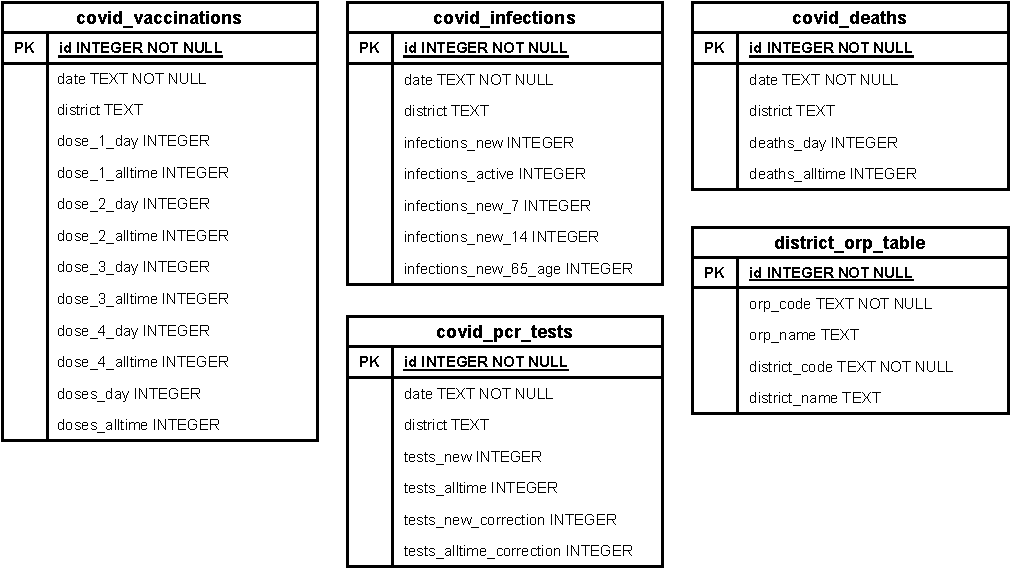
\includegraphics[width=0.87\textwidth]{Pictures/entity.pdf}
	\caption{Schéma databázových tabulek}
	\label{fig:EntityRelationshipDiagram}
\end{figure}

\subsubsection*{Práce s~databází}

Veškerá logická část aplikace, která pracuje s~databází, se nachází v~souboru \emph{database.py}. V~tomto souboru je obsažena singleton třída \lstinline{SQLiteDatabase}, která slouží jako prostředník mezi databází samotnou a~aplikací. Tato třída obsahuje metody, které získávají záznamy z~databáze nebo do databáze záznamy vkládají. Tyto metody přijímají a~vracejí objekty typu \lstinline{CovidVaccinationDayDistrict}, \lstinline{CovidDeathDayDistrict}, \lstinline{CovidInfectionDayDistrict} a~\lstinline{CovidPcrTestDayDistrict}, které reprezentují samotné záznamy v~databázi. Součástí třídy jsou i~metody, které zajišťují připojení k~databázi a~odpojení. Důležitou metodou je metoda \lstinline{commit}, která potvrzuje veškeré změny provedené v~databázi. Tuto metodu je potřeba volat po provedení změn neboť je databáze nastavena tak, že se její změny nepotvrzují automaticky. S~databází se pracuje při zjišťování aktuálnosti dat, aktualizaci dat a~při načítání cache.

\subsection{Stažení nových dat z~API Onemocnění aktuálně a~ukládání}

Při každém přístupu k~webové aplikaci se kontroluje aktuálnost stažených dat. Pokud aplikace zjistí, že data nejsou aktuální, stáhne nová data. Na základě stažených dat se sestaví objekty, které strukturově odpovídají záznamům v~dané databázové tabulce. Poté jsou tyto objekty postupně předány instanci třídy \lstinline{SQLiteDatabase}, která dokáže vložit data do databáze. Vždy se stahují data stará jeden týden, protože během tohoto týdne dochází k~různým korekcím a~opravám na straně API Onemocnění aktuálně. Třída \lstinline{Updater} v~souboru \emph{updater.py} obsahuje statickou metodu \lstinline{update_data}, která stahování dat provádí. Metoda se automaticky volá při přístupu na Django zobrazení \emph{main}. Vzorový požadavek na data z~API Onemocnění aktuálně lze spatřit v~kódu \ref{src:PythonListing}.

Databáze uchovává čtyři kategorie covidových dat - infekce, očkování, úmrtí a~PCR testování. Tyto kategorie mají podobný průběh stažení a~ukládání do databáze. Vždy se zkontroluje, zda nejnovější záznam v~databázi aktuálního datasetu je aktuální, to znamená, že záznam je přesně týden starý. Pokud není, tak aplikace spočítá kolik dní nejsou data aktuální a~pro všechny chybějící dny stáhne nová data. Seznam využitých datasetů se nachází v~kapitole \ref{sec:onemocneni-aktualne}. Dodatečně ještě probíhá kontrola, zda je právě po deváté hodině ráno, protože nová data začne API poskytovat přibližně před devátou hodinou dopoledne. Znázorněný obecný postup stahování dat ve formě diagramu je k~dispozici v~příloze \ref{fig:Diagram2}.

\subsubsection*{Infekce}

Dataset \emph{obce}, i~přes svůj název, obsahuje informace i~o~okrese, jak lze vidět v~příkladu odpovědi API \ref{src:APIinfectionsExample}. Před procházením záznamů se vytvoří prázdný slovník, který slouží jako dočasná úschovna dat okresů. Slovník má v~původním stavu nulové hodnoty, při procházení záznamů (obcí) se hodnoty přičítají k~hodnotě okresu ve slovníku. Jakmile procházení záznamů skončí, z~každého okresu ve slovníku se vytvoří nový objekt, který reprezentuje záznam v~tabulce, a~nahraje se do databáze. Ačkoli dataset \emph{obce} obsahuje počet aktivních případů, aplikace s~tímto počtem pracovat nebude, protože z~neznámého důvodu součet všech aktivních případů obcí pro okres neodpovídá reálnému výsledku.

\clearpage

\begin{lstlisting}[language=Java,label=src:APIinfectionsExample,caption={Schéma vrácených dat z datasetu \emph{obce} z API Onemocnění aktuálně}]
[
  {
    "id": "string",
    "den": "string",
    "datum": "yyyy-MM-dd",
    "kraj_nuts_kod": "string",
    "kraj_nazev": "string",
    "okres_lau_kod": "string",
    "okres_nazev": "string",
    "orp_kod": 0,
    "orp_nazev": "string",
    "obec_kod": 0,
    "obec_nazev": "string",
    "nove_pripady": 0,
    "aktivni_pripady": 0,
    "nove_pripady_65": 0,
    "nove_pripady_7_dni": 0,
    "nove_pripady_14_dni": 0
  }
]
\end{lstlisting}

\subsubsection*{Očkování}

Data očkování jsou na úrovni obcí s~rozšířenou působností (ORP), takže bude potřeba provést určitý převod na okresy. Ve vzorovém vráceném výsledku API Onemocnění aktuálně \ref{src:APIvacExample} lze vidět, že je obsažen klíč \texttt{orp\_bydliste\_kod} s~hodnotou kódu ORP. Tento kód můžeme díky číselníku v~kapitole \ref{sec:ciselnik-orp} převést na okres. Podobně jako u~předchozího datasetu se vytváří prázdný slovník. Tentokrát se ale do slovníku nahrají hodnoty z~předchozího dne, které reprezentují celkové dosavadní počty. Denní počty jsou v~původním stavu nulové. Poté se prochází všechny vrácené záznamy z~API. Každý záznam reprezentuje danou dávku v~ORP, obsahem jednoho záznamu je počet vydaných daných dávek, např. pořadí dávky je 2 a~počet dávek je 10, tudíž bylo vydáno 10 druhých dávek v~této ORP. Hodnoty záznamů se postupně ukládají do slovníku, kde se na závěr převede každý klíč a~hodnota na objekt reprezentující záznam v~tabulce, jež se poté nahraje do databáze.

\clearpage

\begin{lstlisting}[language=Java,label=src:APIvacExample,caption={Schéma vrácených dat z datasetu \emph{ockovani-geografie} z API Onemocnění aktuálně}]
[
  {
    "id": "string",
    "datum": "yyyy-MM-dd",
    "vakcina": "string",
    "vakcina_kod": "string",
    "poradi_davky": 0,
    "kraj_nazev": "string",
    "kraj_nuts_kod": "string",
    "orp_bydliste": "string",
    "orp_bydliste_kod": 0,
    "pocet_davek": 0
  }
]
\end{lstlisting}

\subsubsection*{Úmrtí}

V~případě dat o~úmrtí se využívá dataset \emph{umrti}, který poskytuje základní informace o~zemřelém člověku (viz. vrácený výsledek \ref{src:APIdeathsExample}). Stejně jako ve všech ostatních datasetech se vytváří slovník pro úschovnu dat okresů a~ukládají se do něj nulové denní počty a~celkové dosavadní počty z~předchozího dne. Každý záznam z~API reprezentuje jednoho zemřelého člověka. Díky tomu, že záznam obsahuje klíč \texttt{okres\_lau\_kod}, můžeme úmrtí přiřadit k~danému okresu ve slovníku. V~poslední řadě se výsledky nahrají do databáze.

\begin{lstlisting}[language=Java,label=src:APIdeathsExample,caption={Schéma vrácených dat z datasetu \emph{umrti} z API Onemocnění aktuálně}]
[
  {
    "id": "string",
    "datum": "yyyy-MM-dd",
    "vek": 0,
    "pohlavi": "string",
    "kraj_nuts_kod": "string",
    "okres_lau_kod": "string"
  }
]
\end{lstlisting}

\subsubsection*{PCR testování}

Na závěr se používá dataset \emph{kraj-okres-testy} pro získání dat o~provedených PCR testech v~okresech. Vzorový záznam tohoto datasetu lze vidět v~kódu \ref{src:APItestsExample}. Práce s~datasetem je velice jednoduchá neboť obsahuje veškeré potřebné informace o~počtu testů pro daný den a~kumulativních celkových počtech pro všechny okresy. Aplikace tak pouze stáhne data pro chybějící dny a~pro každý tento den iteruje vrácenými záznamy, jež si ukládá do dočasného slovníku, který na závěr po převedení na dané objekty nahraje do databáze.

\begin{lstlisting}[language=Java,label=src:APItestsExample,caption={Schéma vrácených dat z datasetu \emph{kraj-okres-testy} z API Onemocnění aktuálně}]
[
  {
    "id": "string",
    "datum": "yyyy-MM-dd",
    "kraj_nuts_kod": "string",
    "okres_lau_kod": "string",
    "prirustkovy_pocet_testu_okres": 0,
    "kumulativni_pocet_testu_okres": 0,
    "prirustkovy_pocet_testu_kraj": 0,
    "kumulativni_pocet_testu_kraj": 0,
    "prirustkovy_pocet_prvnich_testu_okres": 0,
    "kumulativni_pocet_prvnich_testu_okres": 0,
    "prirustkovy_pocet_prvnich_testu_kraj": 0,
    "kumulativni_pocet_prvnich_testu_kraj": 0
  }
]
\end{lstlisting}

\subsection{API pro komunikaci s~klientem}

\subsubsection*{Typ API}

Pokud chcete v~Django projektu vytvořit vlastní API, pravděpodobně se setkáte s~implementací pomocí REST API. Tento způsob umožňuje vytvořit webové API, které dokáže přistupovat k~datům uvnitř aplikace. V~Djangu lze REST API vytvořit pomocí knihovny Django REST framework. Tato knihovna nabízí podporu pro autentizaci, autorizaci a~řízení přístupu k~datům, dokáže generovat dokumentaci pro API a~mnoho další \cite{rest-api}.

I~když by se REST API mohlo zdát jako vhodná volba pro implementaci API v~naší aplikaci, v~našem konkrétním případě to není nutné. API v~této nové aplikaci je velice jednoduché a~nenáročné, je potřeba pouze stáhnout data bez kontroly uživatele. Také není nutné naše data nějak chránit, jedná se totiž o~data, která jsou volně přístupná. API v~této aplikaci bude stavěno na jednom upraveném zobrazení, které bude voláno při přístupu na danou URL s~parametry.

V~kapitole \ref{sec:webframework} byla lehce popsána struktura frameworku Django a~bylo zmíněno, že v~souboru \emph{urls.py} se mapují URL adresy ke konkrétním zobrazením. Tato URL mohou také přijímat parametry ve formátu, který lze vidět v~kódu \ref{src:DjangoAPIUrl}. Každý parametr je ohraničen znaménky větší než a~menší než a~uvnitř těchto znamének je specifikovaný datový typ parametru společně s~jeho názvem. Samotné parametry jsou předány do parametrů funkce zobrazení, tyto parametry musí mít stejný název jak v~URL, tak i~ve funkci. 

\begin{lstlisting}[language=Python,label=src:DjangoAPIUrl,caption={Mapování URL k API}]
urlpatterns = [
    path('api/from=<str:range_from>&to=<str:range_to>', covid.views.api, name='api')
]
\end{lstlisting}

Jelikož se jedná o~API (velice zjednodušené), bude dané zobrazení vracet výsledek ve formátu JSON. Pro docílení vrácení JSONu je nutné v~zobrazení vracet \lstinline{JsonResponse} namísto standardní HTML stránky.

\subsubsection*{Workflow API}

API přijímá na své jediné URL adrese dva parametry - jedná se o~časové rozmezí od a~do. Ještě než se získají data na základě časového rozmezí, zkontroluje se, zda se uživatel nedotazuje na data příliš často (viz. následující podkapitola \ref{APIsecurity}). Po této kontrole se volá metoda \lstinline{get_data} třídy \lstinline{Cache}, které jsou předány parametry, a~ty zkontroluje, zda jsou validní. Pokud dojde k~chybě parametrů, API vrátí výsledek s~chybovým HTTP kódem 400, který znamená špatný požadavek. Pokud jsou parametry validní, zpracují se z~cache výsledná data. Získaná data z~cache se následně komprimují za pomocí knihovny zlib a~komprimovaný výsledek se vrátí klientovi (porovnání velikostí komprimovaného a~nekomprimovaného slovníku a~rychlosti odpovědí lze vidět v~grafech \ref{fig:Compress}).

\begin{figure}[h]
\centering
\subfloat[Porovnání velikostí slovníku]{\label{fig:CompressSize}{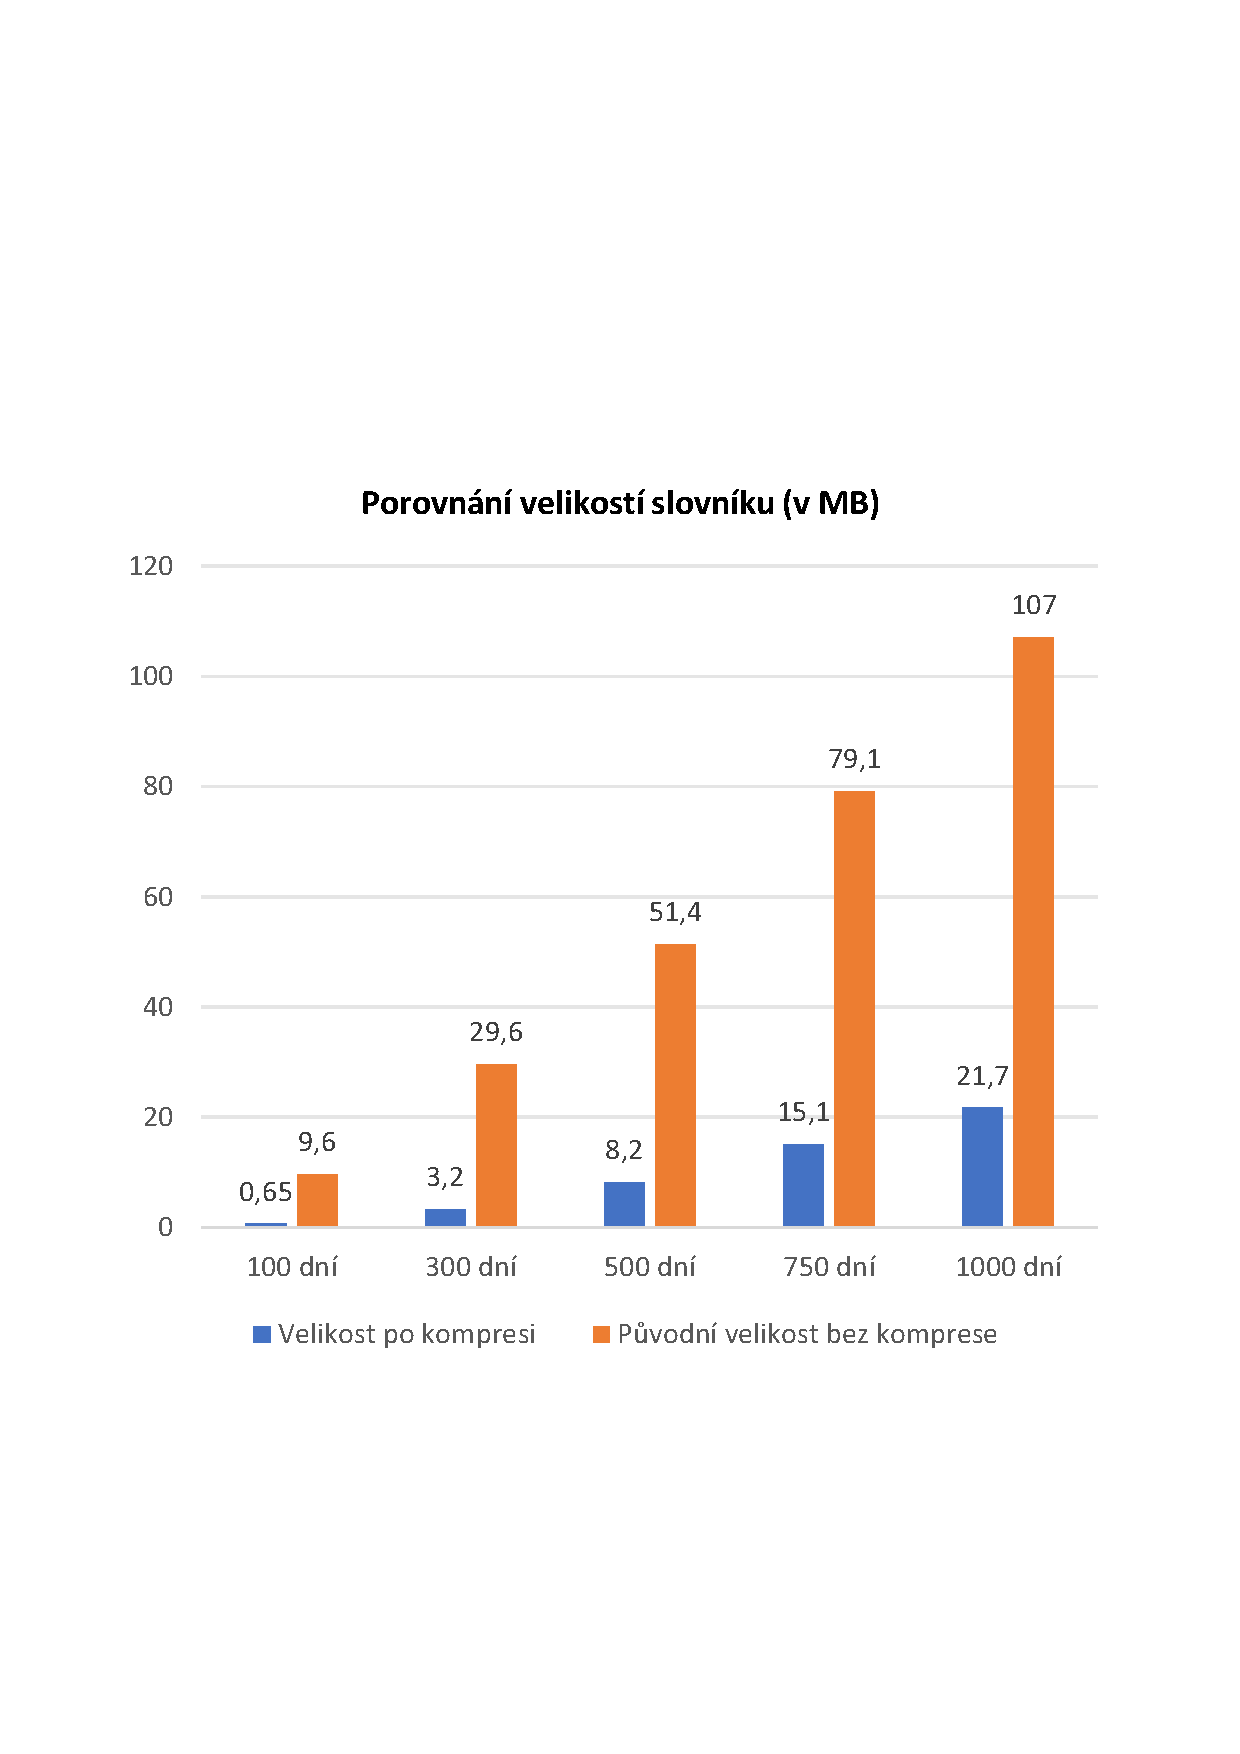
\includegraphics[width=0.47\textwidth]{Pictures/Graf1_crop.pdf}}}\hfill
\subfloat[Porovnání rychlostí odpovědi na lokálním serveru]{\label{fig:CompressTime}{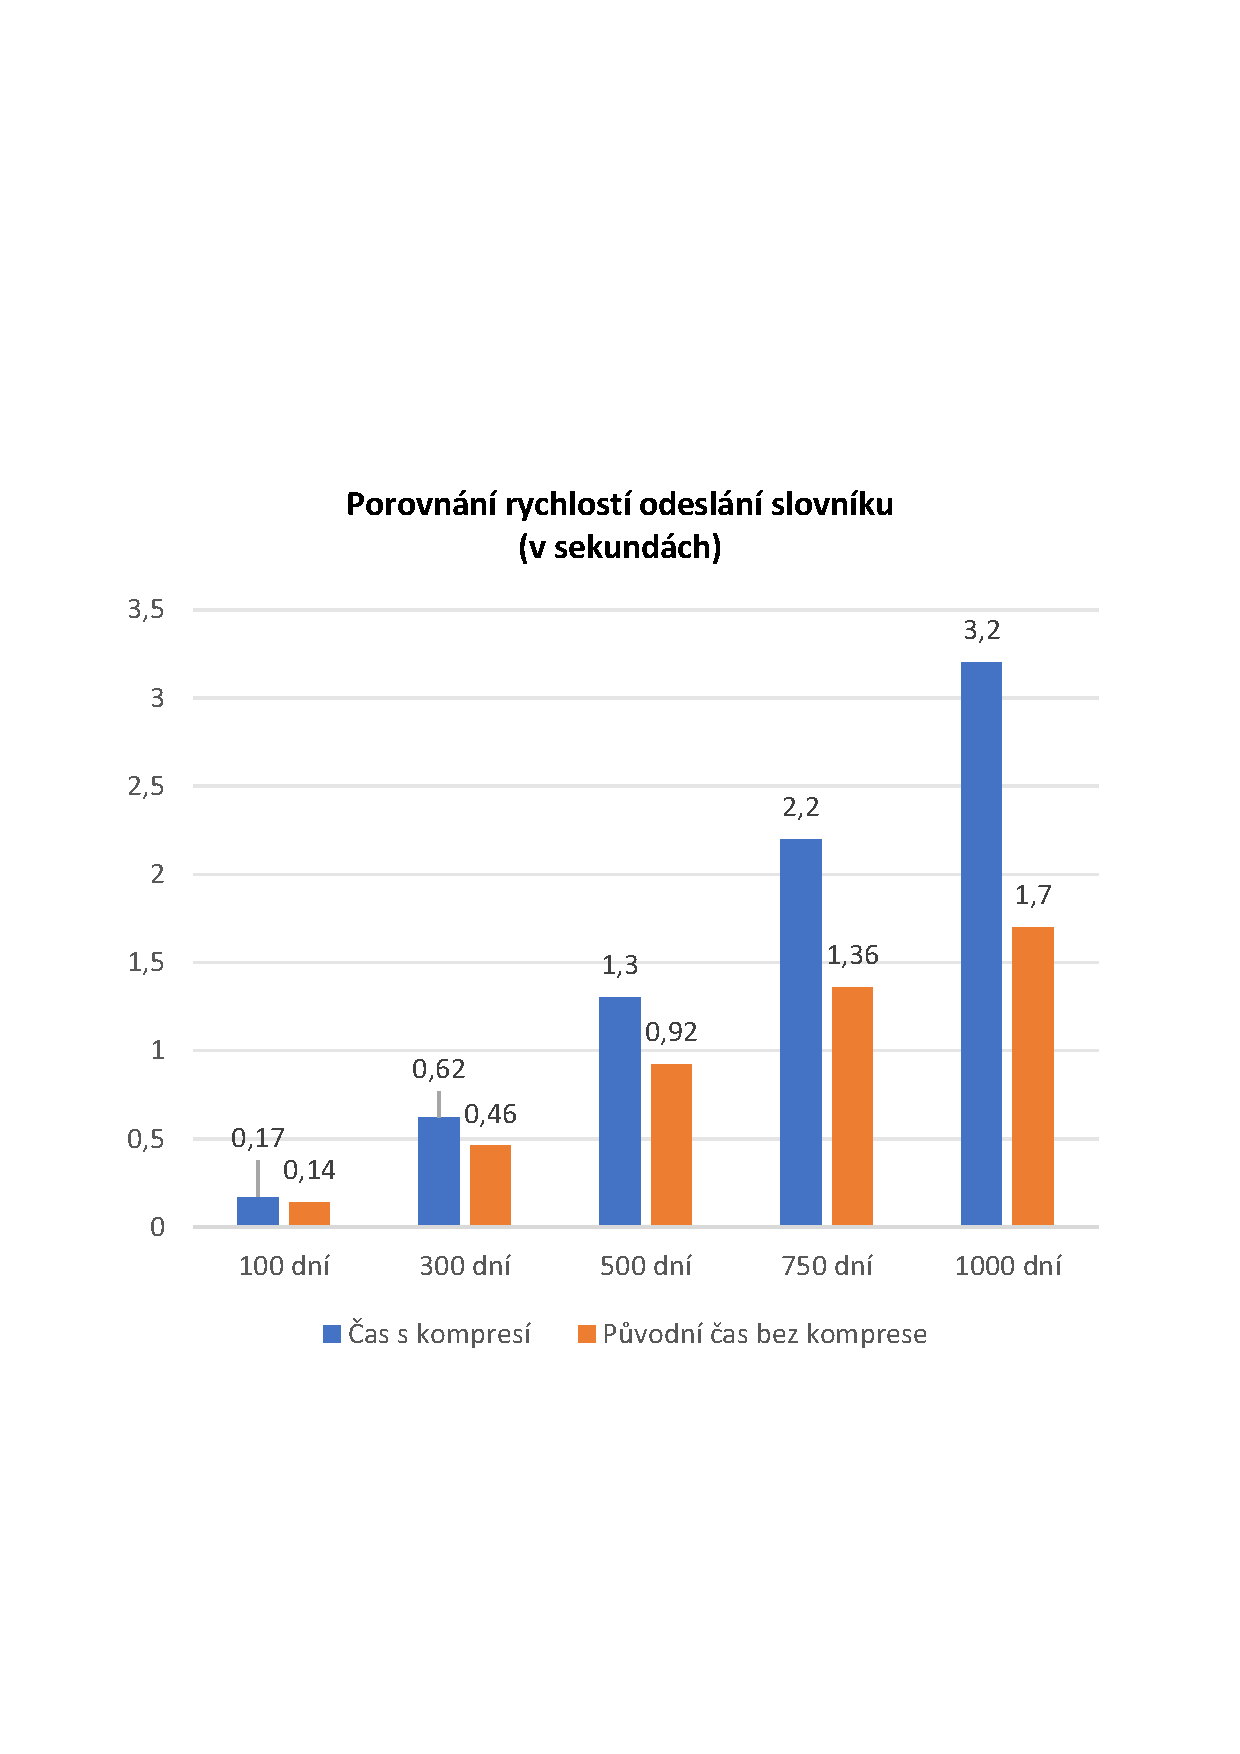
\includegraphics[width=0.47\textwidth]{Pictures/Graf2_crop.pdf}}}
\caption{Porovnání původních dat a~komprimovaných}
\label{fig:Compress}
\end{figure}

\subsubsection*{Kontrola zahlcení uživatelem}
\label{APIsecurity}
Aplikace sleduje IP adresy, ze kterých jsou HTTP požadavky odesílány. To je realizováno sledováním hlaviček \emph{HTTP\_X\_FORWARDED\_FOR} a \emph{REMOTE\_ADDR}, které mohou obsahovat IP adresu klienta, jež zaslal požadavek. Tyto hlavičky jsou obsaženy v~Django objektu \lstinline{HttpRequest}, který se automaticky předává zobrazení. Každý uživatel může přistoupit k~API pouze jednou za 20 sekund za~účelem zamezení zahlcení serveru. O~tuto funkčnost se stará statická metoda \lstinline{allow_request}, která je součástí třídy \lstinline{ClientAPI}, v~souboru \emph{api.py}. Tato metoda kontroluje, zda je daná IP adresa obsažena ve slovníku uchovaných IP adres. Pokud je obsažena, zkontroluje se její hodnota, která odpovídá času posledního přístupu k~API. Jakmile je rozdíl časů více jak 20 sekund, přístup je povolen, v~opačném případě se odešle zpět odesílateli výsledek s~chybovým HTTP kódem 429. Pokud není IP adresa ve slovníku, je přístup uživateli povolen a~čas přístupu je nově zaznamenán do slovníku.

Celý proces stahování dat z~API aplikace je dostupný v~příloze \ref{fig:Diagram1} ve formě diagramu.

\subsection{Cachování}
\label{cache}

Aplikace na straně serveru je schopna tzv. cachování. Cachování je proces ukládání dat do takové paměti, která je snadno dostupná a~rychlejší, než samotný zdroj poskytující daná data. Cílem je snížit počet I/O operací (čtení a~zápis dat) pomalejších disků a~urychlit přístup k~datům \cite{auth0-caching}.

Veškerá funkcionalita cachování je ukryta v~souboru \emph{cache.py}, kde se nachází singleton třída \lstinline{Cache}, která obsahuje metody pro ukládání do cache \lstinline{update_data} a~načítání z~cache \lstinline{get_data}. Při startu aplikace se ve frameworku Django automaticky vytváří instance třídy \lstinline{Cache} a~poté se cache naplní. Proces funguje tak, že se získají všechny dny v~databázi a~uloží se do velkého slovníku, který je uložený v~paměti RAM. Při ukládání dat do slovníku se také počítají maximální nalezené hodnoty v~dnech pro každý typ dat ve všech datasetech a~to z~toho důvodu, že aplikace poskytuje možnost škálovat zobrazení dat podle největší nalezené hodnoty. Díky těmto datům je poté snazší najít maximální hodnoty v~daném časovém období, které si uživatel zvolí. Celý proces cachování trvá přibližně 20-30 sekund (ve virtualizovaném stroji s~CPU AMD Ryzen 7 5800H a~NVMe diskem) a~nově utvořený slovník zabírá v~paměti RAM přibližně 110 MB (všechna data do 16.3.2023 - 1063 dní). 

Aplikace je připravena na aktualizaci cache v~případě, že dojde k~neaktuálnosti dat. V~tomto případě dokáže metoda \lstinline{update_data} přijmout parametr se seznamem dní, které má nově vložit z~databáze do existujícího slovníku, a~tak dojde k~aktualizaci cache za běhu. Metoda \lstinline{update_data} je volána vždy, když instance třídy \lstinline{Updater} zjistí, že jsou data neaktuální.

Při žádosti o~data z~našeho API dojde k~volání metody \lstinline{get_data}, která přijímá dva parametry, a~to časové rozpětí ve formě data od a~do. Toto rozpětí aplikace projde a~získá si potřebné dny, každý den si poté zkopíruje z~cache do nového slovníku společně s~dopočtenými maximálními hodnotami. Aplikace při výpočtu dní kontroluje, zda je rozpětí platné, to znamená, že není datum v~parametru od \enquote{větší} než parametr do a~naopak. Pokud se tak stane, aplikace vrátí chybový HTTP kód 400. Stejný kód aplikace vrátí, když daný den nebyl v~cache nalezen nebo pokud se nejedná o~validní datum.

\section{Popis důležitých komponent a~částí frontendu}

Součástí této podkapitoly jsou popisy a~vysvětlení různých důležitých komponent a~částí aplikace na straně uživatele. Aplikace využívá několik knihoven pro zlepšení uživatelského rozhraní. Díky některým knihovnám je možné použít v~aplikaci interaktivní grafy a~jiné interaktivní prvky. Většina logické části frontendu se nachází v~souboru \emph{core.js}.

\subsection{Uživatelské rozhraní}
\label{gui}

Uživatelské rozhraní (UI) je způsob, jakým uživatelé interagují s~počítačem, aplikací nebo jiným zařízením. Jedná se o~soubor prvků a~funkcí, které umožňují uživatelům komunikovat s~technologií a~provádět požadované úkoly.

Velkou část aplikace na straně klienta tvoří grafické uživatelské rozhraní (GUI). GUI se obvykle skládá z~vizuálních prvků, které umožňují uživatelům interagovat s~webovými stránkami pomocí myši, klávesnice nebo dotykové obrazovky. Správné používání GUI na webových stránkách může pomoci uživatelům snadno se orientovat na stránce a~snadněji používat aplikaci. 

Návrh uživatelského rozhraní lze vidět v~podkapitole \ref{uisample}. Mezi hlavní prvky aplikace patří vrchní lišta s~přepínači datasetů a~tmavého režimu. Jakmile si uživatel zvolí dataset, po celém rozhraní se aplikuje barevné schéma reprezentující daný dataset (zelená, fialová, šedá a~oranžová). Důležitým prvkem je levé okno s~nastavením aplikace. V~tomto okně uživatel nalezne volbu časového okna, úpravu vizualizace a~nastavení zobrazovaných dat a~animace. Mezi vedlejší prvky patří spodní levé okno s~obecným textem o~zobrazovaných datech a~škálou barev, pravé horní okno s~obrazem v~obraze (PiP) a~pravé spodní okno s~grafem. Okna s~obrazem v~obraze a~grafem se dají skrýt, pokud si to uživatel přeje, a~levé spodní okno lze zmenšit. Na závěr se může zobrazovat drobné \enquote{pop-up} okno při kliknutí nebo přejetím myši na okres. Drobnou součástí GUI jsou také uvítací okna aplikace a~informace o~autorovi.

V~nastavení aplikace v~záložce \emph{Zobrazení} lze měnit škálování uživatelského rozhraní. Je to z~toho důvodu, že zařízení mají různé velikosti obrazovek a~rozlišení, tudíž na některých obrazovkách může být GUI poměrně malé nebo naopak velké. Proto je uživateli umožněno si GUI zmenšit nebo zvětšit podle svých potřeb, uživateli je také při spuštění aplikace zobrazeno oznámení o~možné změně velikosti GUI. Hodnota měřítka GUI se ukládá v~lokálním úložišti prohlížeče, aby nebylo nutné měřítko při dalším přístupu k~aplikaci opět měnit.

Veškeré grafické uživatelské rozhraní této aplikace na straně klienta se nachází v~HTML souboru \emph{index.html}, jež se nachází v~adresáři \emph{templates} ve složce s~Django projektem.

\subsubsection*{Návrh uživatelského rozhraní}
Následující obrázky \ref{fig:WireframeWelcome}, \ref{fig:WireframeDefault} a~\ref{fig:WireframeFull} zobrazují návrh uživatelského rozhraní ve webové aplikaci. Znázorňují úvodní obrazovku a~rozvržení elementů na obrazovce.


\label{wireframes}
\begin{figure}[H]
	\centering
	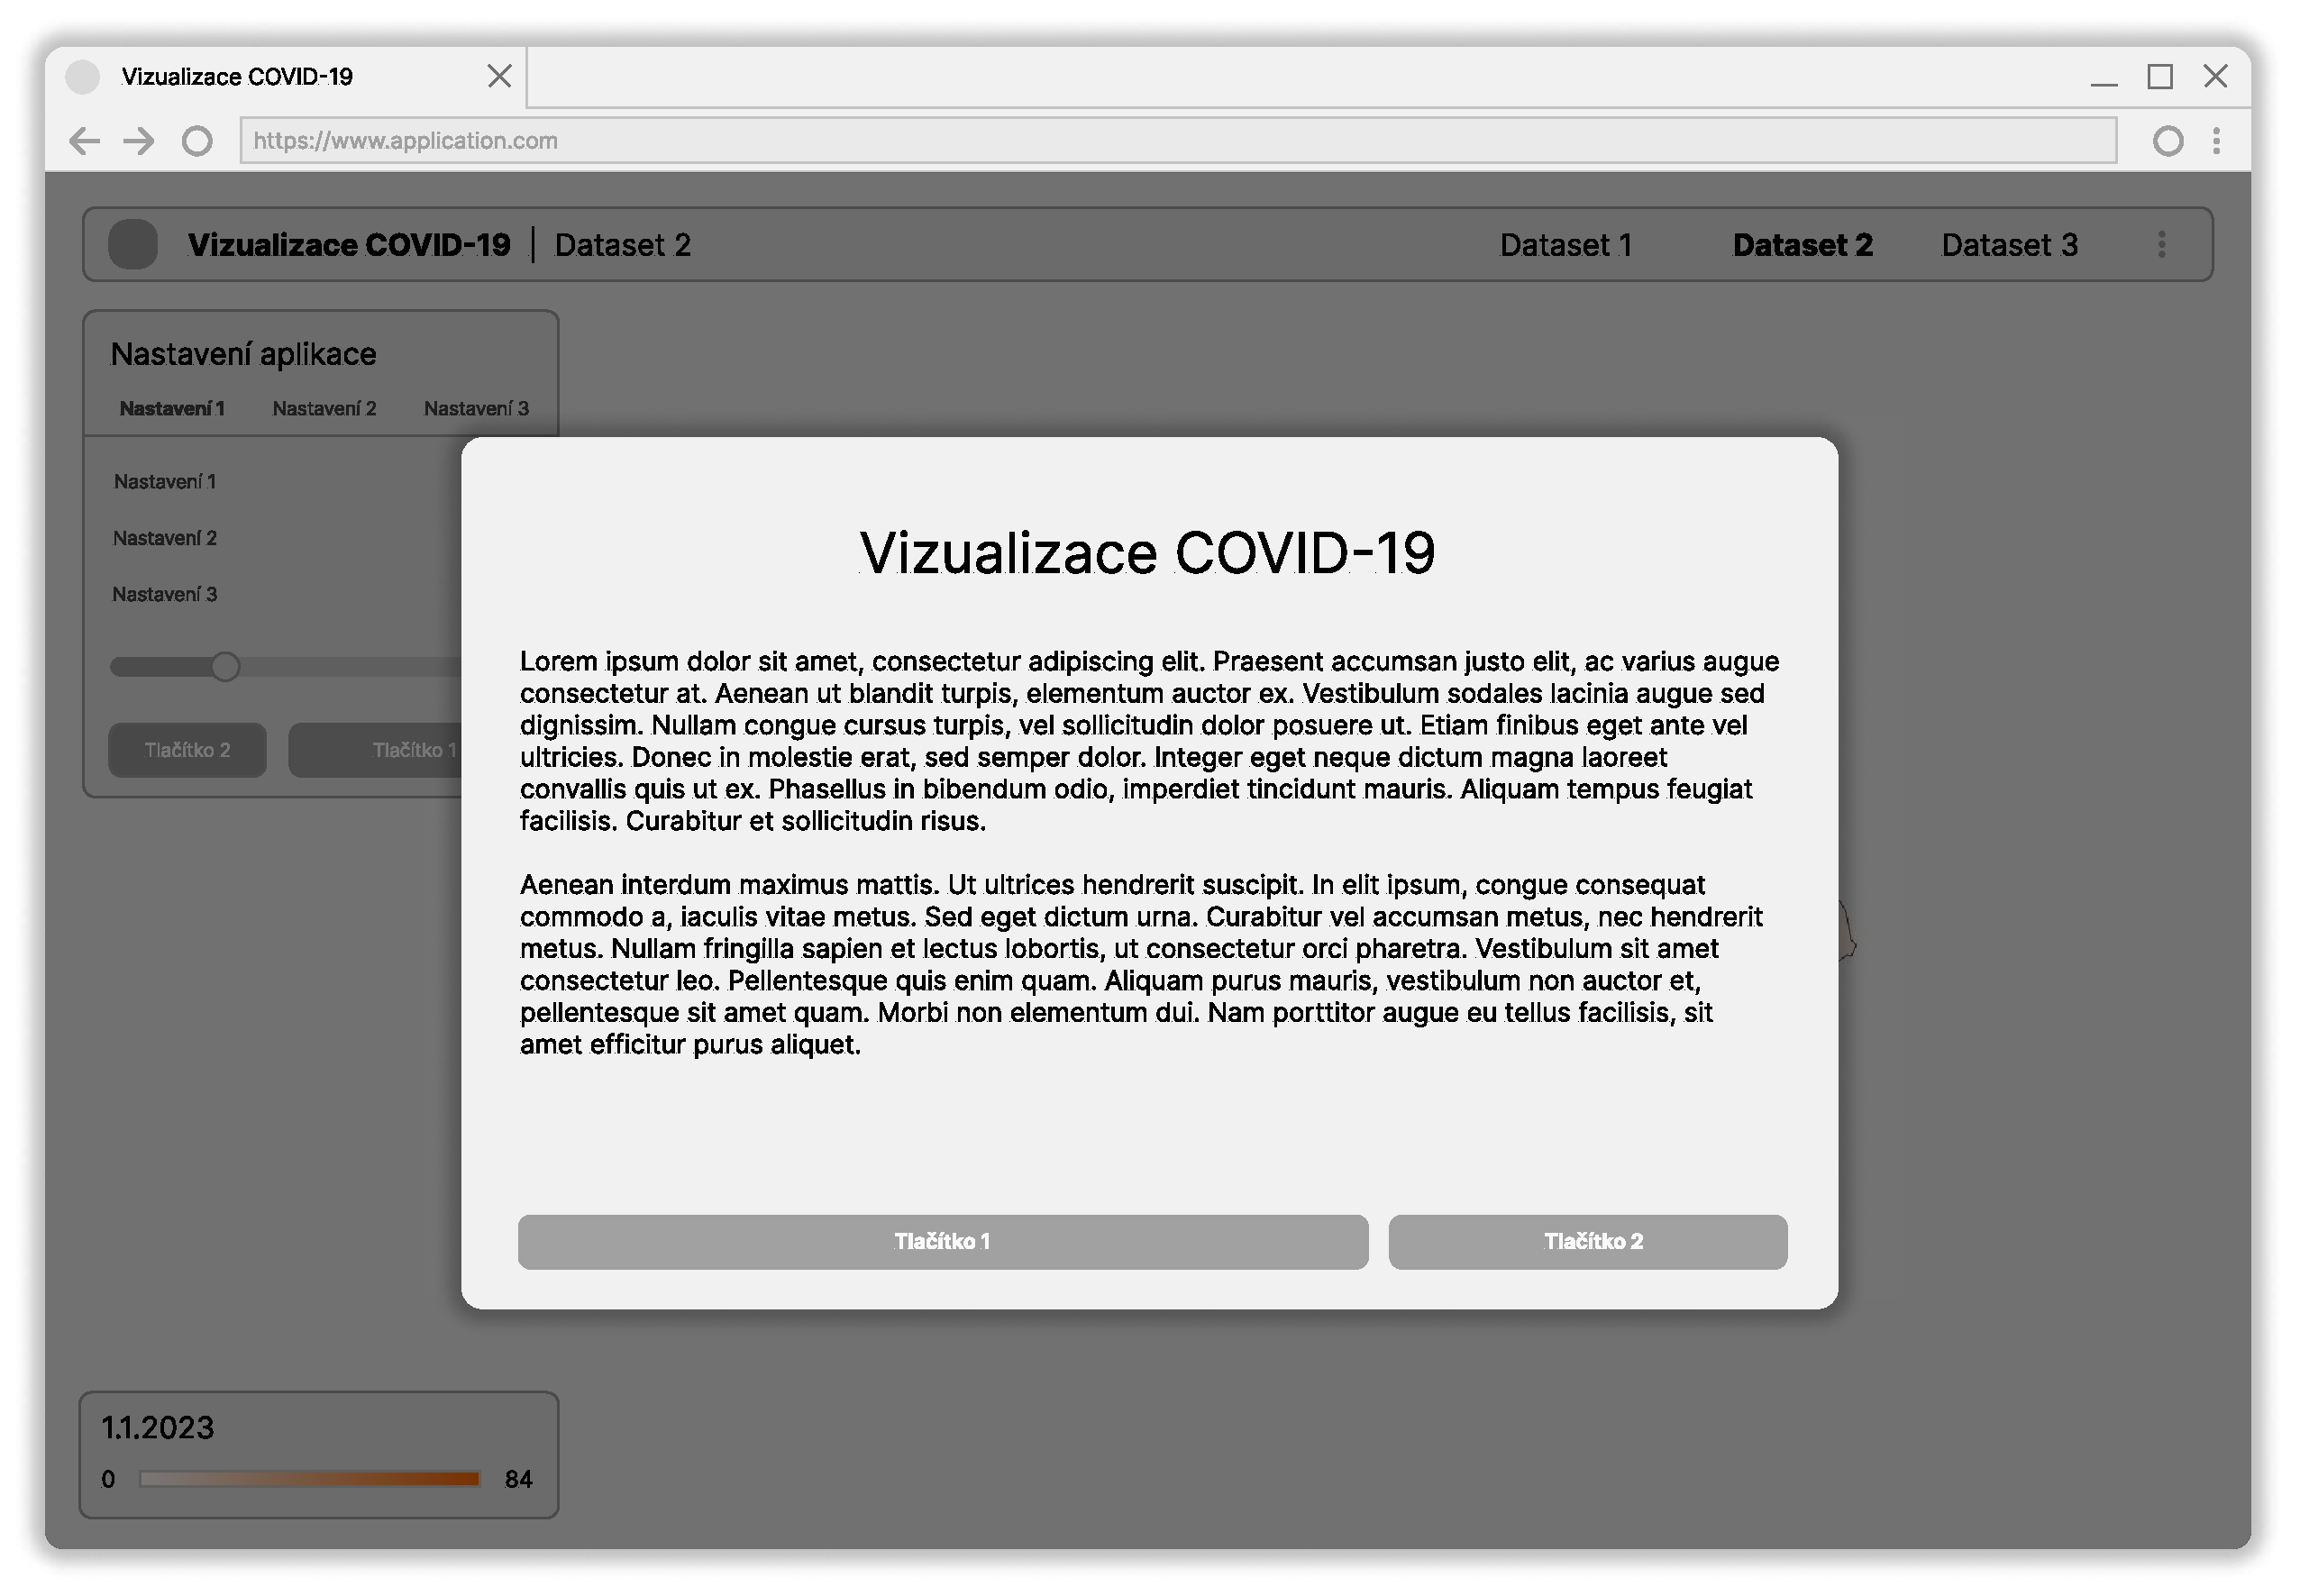
\includegraphics[width=0.85\textwidth]{Pictures/wireframe_welcome.pdf} 
	\caption{Wireframe - úvodní přivítání uživatele ve webové aplikaci}
	\label{fig:WireframeWelcome}
\end{figure}

\begin{figure}[H]
	\centering
	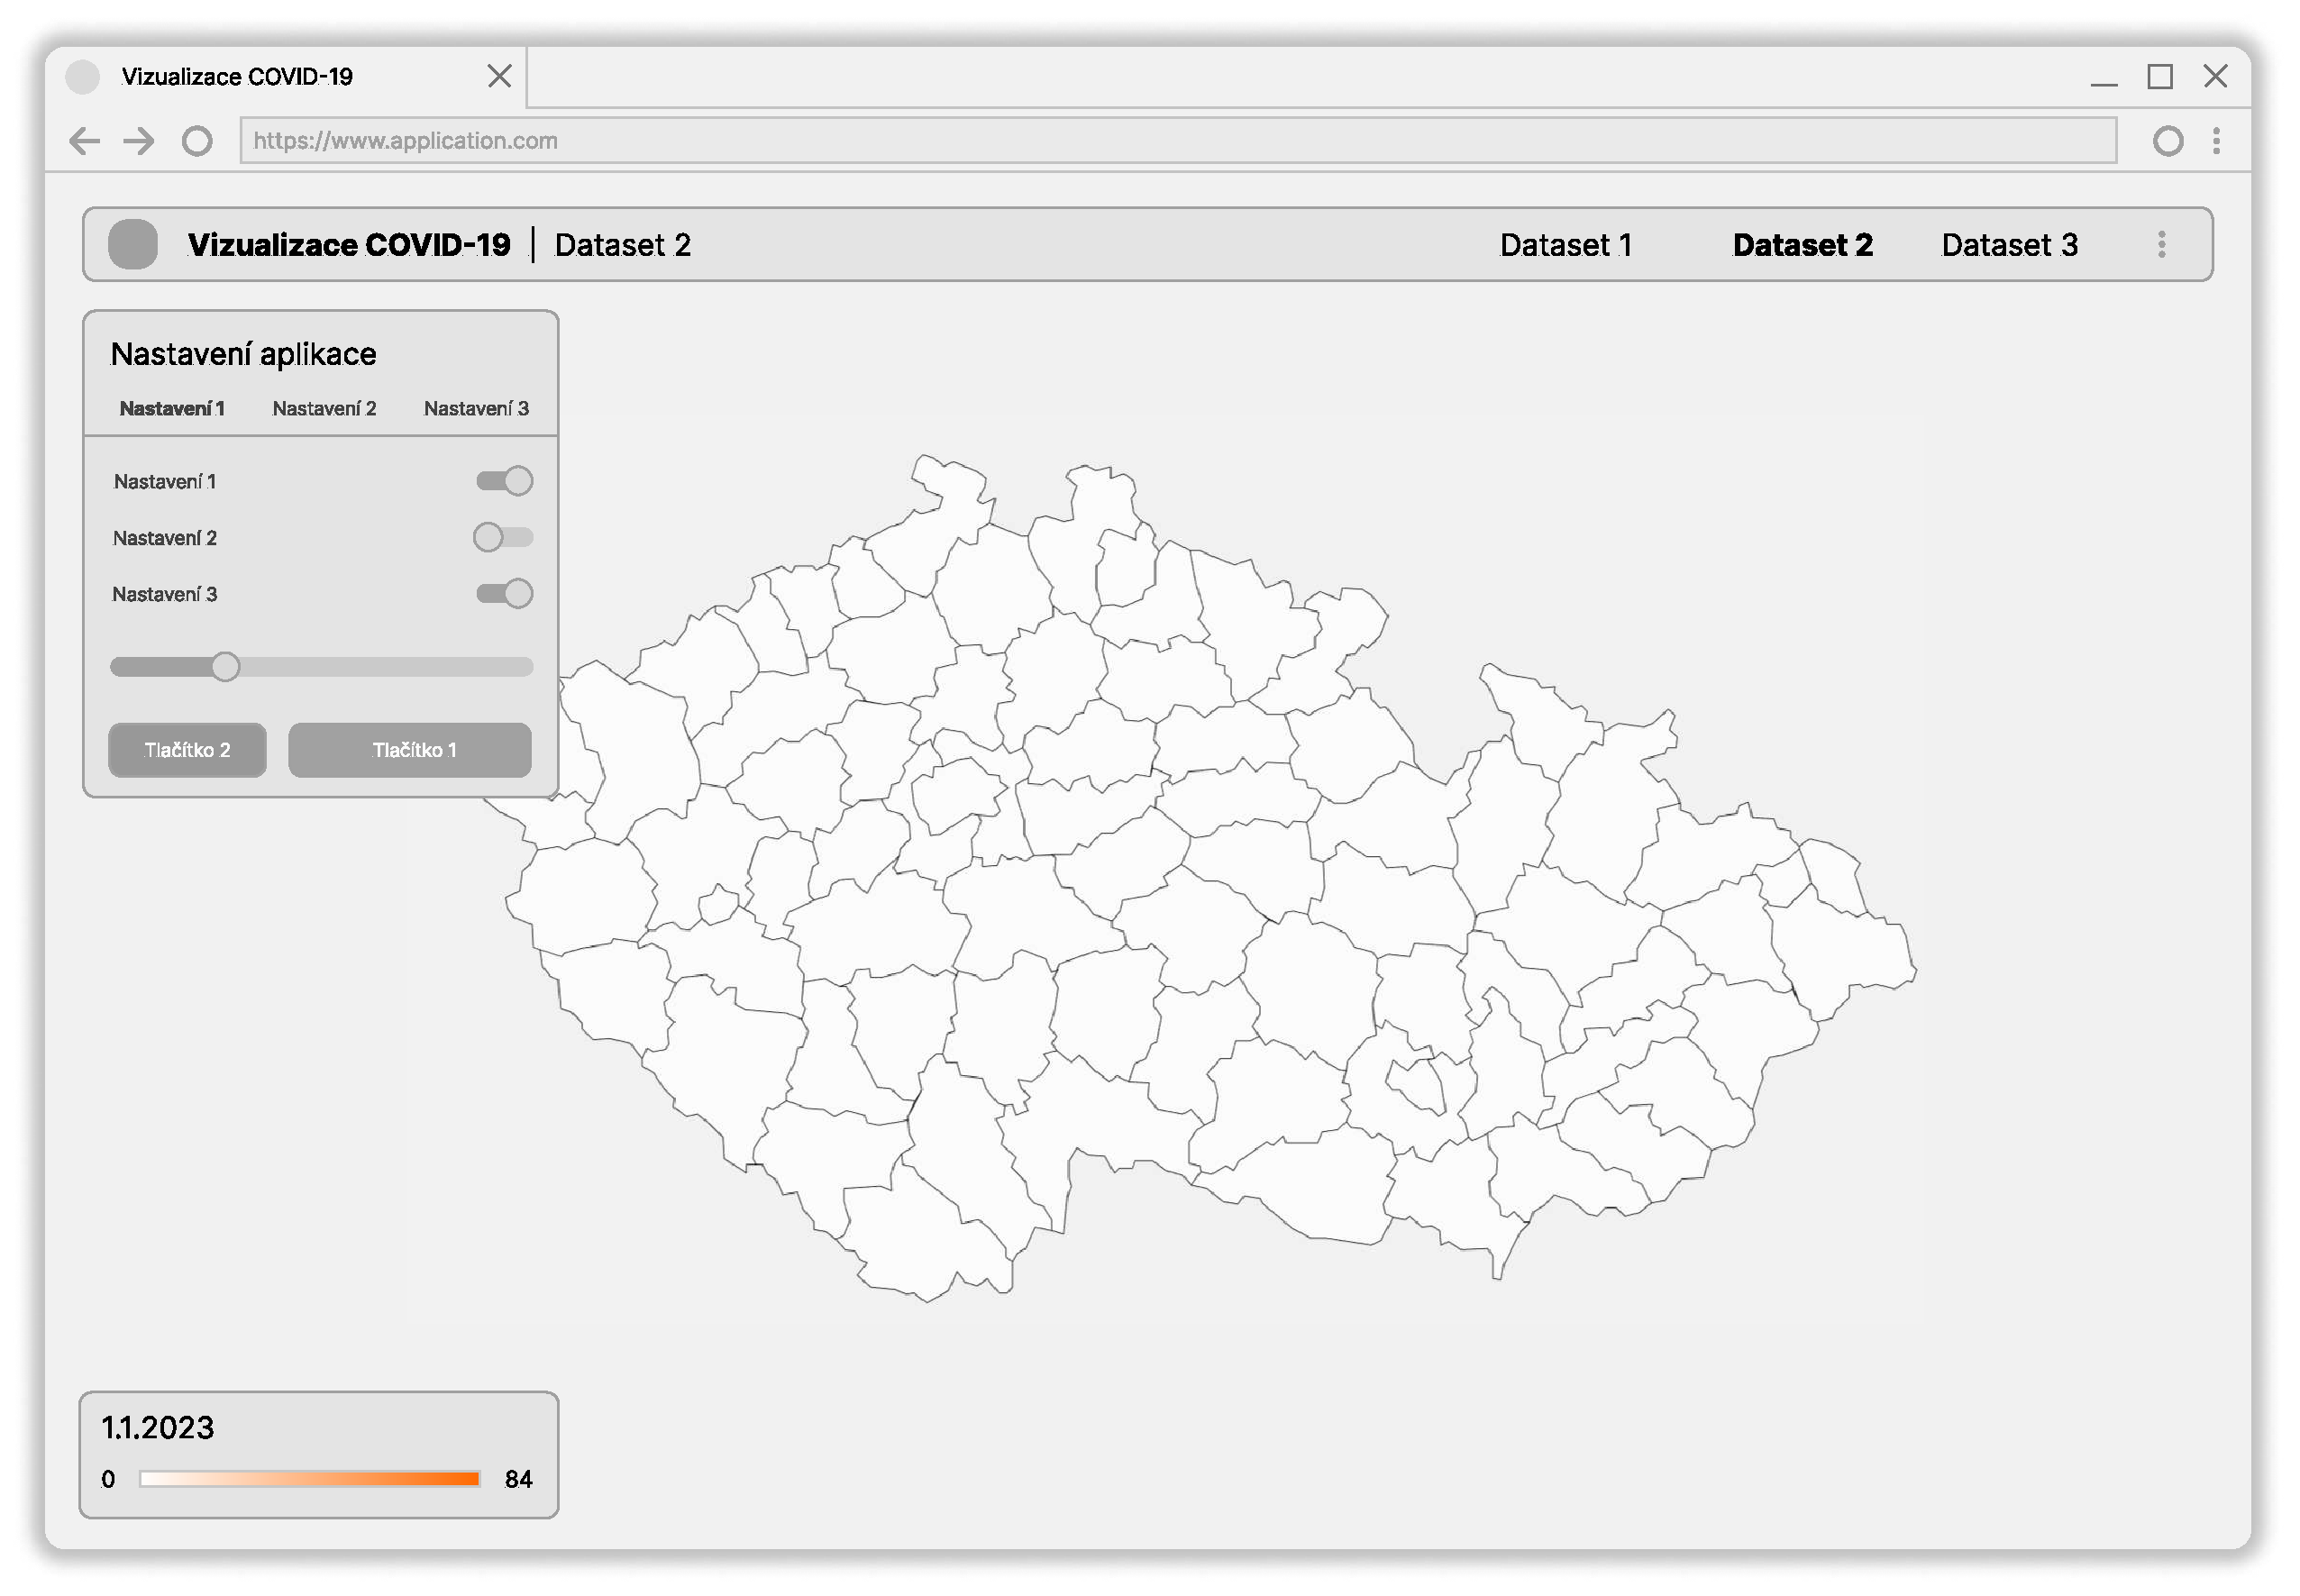
\includegraphics[width=0.85\textwidth]{Pictures/wireframe_default_white.pdf}
	\caption{Wireframe - defaultní prostředí webové aplikace}
	\label{fig:WireframeDefault}
\end{figure}

\begin{figure}[H]
	\centering
	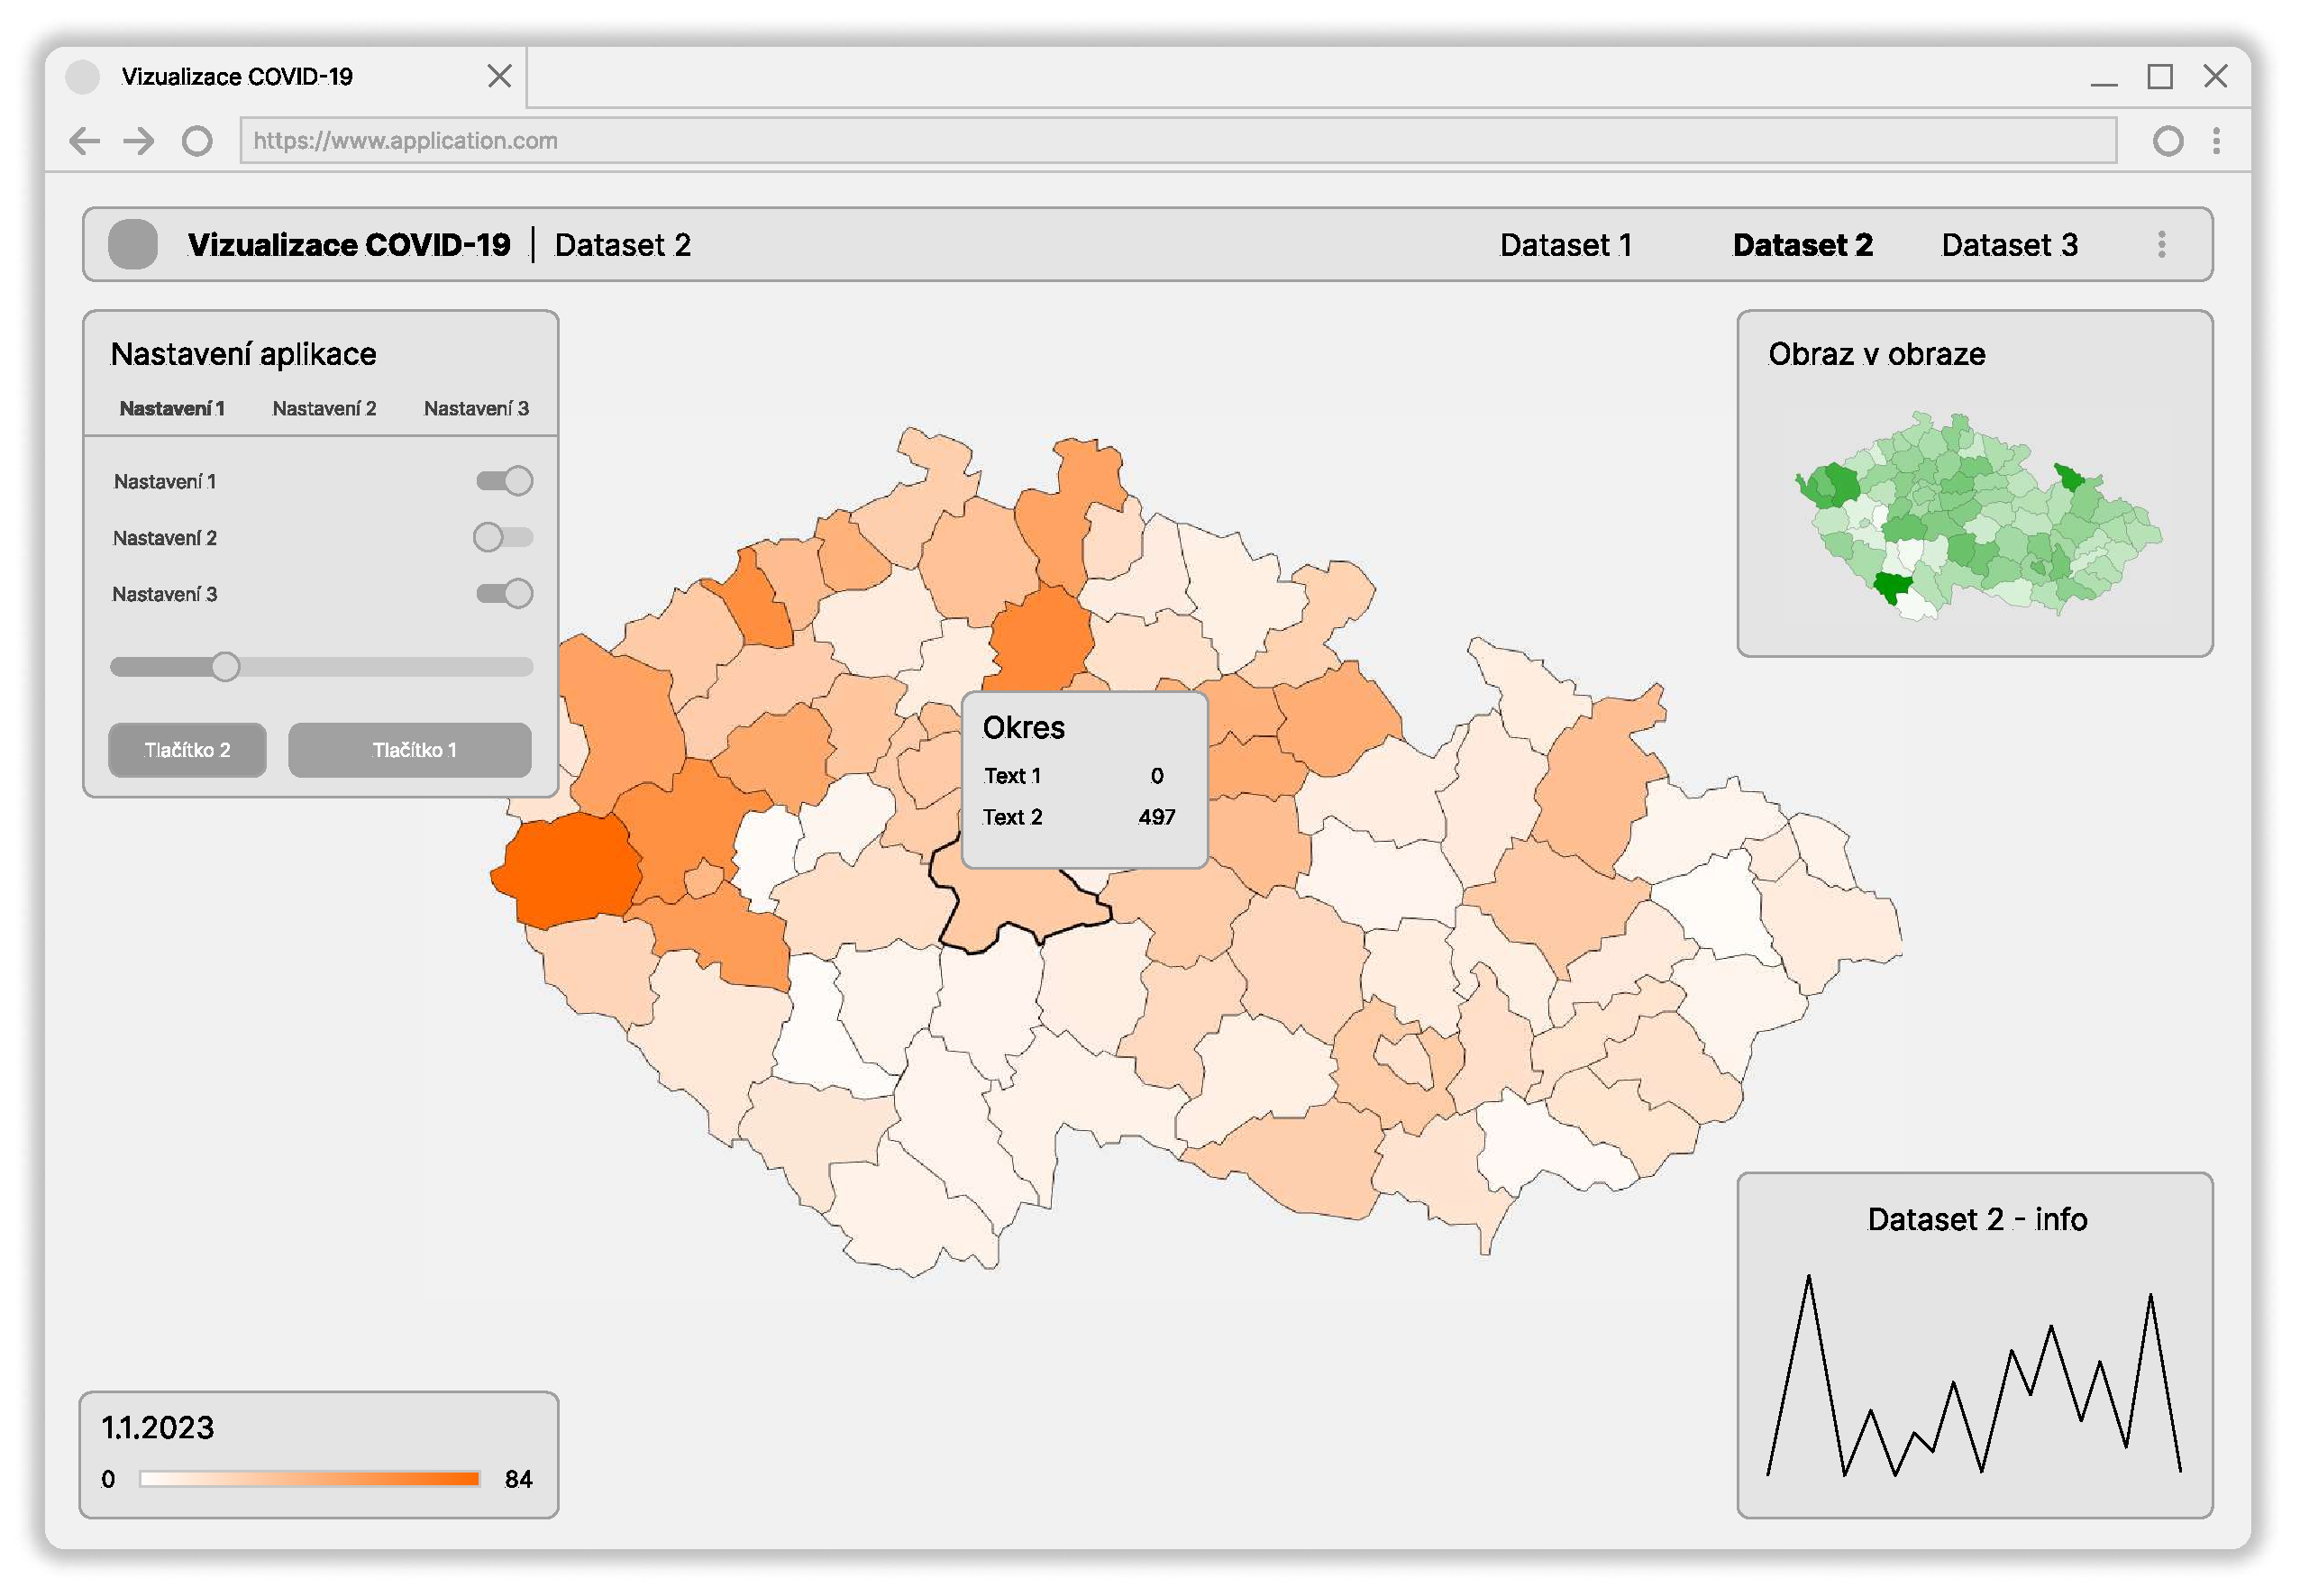
\includegraphics[width=0.85\textwidth]{Pictures/wireframe_full.pdf}
	\caption{Wireframe - detailní analýza okresu ve webové aplikaci}
	\label{fig:WireframeFull}
\end{figure}

\subsubsection*{W3.CSS}

Pro tvorbu kvalitního a~responzivního uživatelského rozhraní existuje mnoho frameworků a~knihoven. V~naší aplikaci byl využit W3.CSS. W3.CSS je moderní CSS framework vyvinutý organizací W3C (World Wide Web Consortium). Tento framework obsahuje mnoho předdefinovaných tříd a~stylů, které umožňují tvorbu moderních a~responzivních webových stránek, a~tak usnadňují programátorovi práci. Práce s~tímto frameworkem je velice jednoduchá a~obsahuje kvalitní dokumentaci s~ukázkovými příklady, navíc je navržen tak, aby fungoval na široké škále zařízení a~při různých velikostech obrazovky.

W3.CSS poskytuje velké množství responzivních prvků, celou dokumentaci lze nalézt zde \cite{w3-css-dokumentace}. Mezi nejpoužívanější třídy tohoto frameworku v~aplikaci patří karty (\texttt{w3-card}), kontejnery \newline(\texttt{w3-container}), zarovnávací třídy (např. \texttt{w3-center} nebo \texttt{w3-padding}) a~tlačítka (\texttt{w3-button}). Velice často také aplikace čerpá z~barevných schémat, které framework poskytuje. Framework dokonce poskytuje i~třídy animací, ty jsou využity např. v~přepínaní stránek nastavení.

Pro použití tohoto frameworku je nutné do HTML stránky vložit odkaz na framework přes element \emph{link}. Tento element se používá k~propojení webových stránek s~externími soubory, jako jsou např. kaskádové styly, JavaScript soubory nebo fonty. Tímto způsobem se používá framework v~naší aplikaci, lze ale framework také používat lokálně a~využít jej offline. Společně s~W3.CSS se do webové stránky přidává odkaz na barevná schémata W3.CSS, která se v~aplikaci využívají.

\subsubsection*{Material Design Lite}

Material Design Lite (MDL) je knihovna webových komponent pro usnadnění vývoje moderních a~responzivních webových stránek. Tato knihovna byla vyvinuta společností Google a~nabízí sadu předdefinovaných stylů a~komponent, které jsou inspirovány konceptem Material Design. Material Design je vizuální jazyk, který byl vyvinut společností Google pro jednotný vzhled a~chování aplikací napříč platformami a~zařízeními \cite{mdl-dokumentace} a~kterým je inspirované celé GUI frontendu.

Nejnovější verze tohoto vizuálního jazyka je 3, bohužel ale není tato verze zatím dostupná pro webové aplikace (v~době vývoje aplikace), je dostupná pouze pro Android aplikace. Naše aplikace tudíž využívá starší verze 2. Ukázku komponent nejnovější verze lze vidět na obrázku \ref{fig:MD3pic}.

Nejčastěji použité prvky z~této knihovny v~naší aplikaci jsou přepínače (\texttt{mdl-switch}), tlačítka (\texttt{mdl-button}) a~je taky využit posuvník (\texttt{mdl-slider}) při vybírání dne z~časového okna. V~poslední řadě je využit tzv. snackbar (\texttt{mdl-snackbar}), jedná se o~informační okno obsahující zprávu pro uživatele, které automaticky po určitém čase zmizí.

\begin{figure}[h]
	\centering
	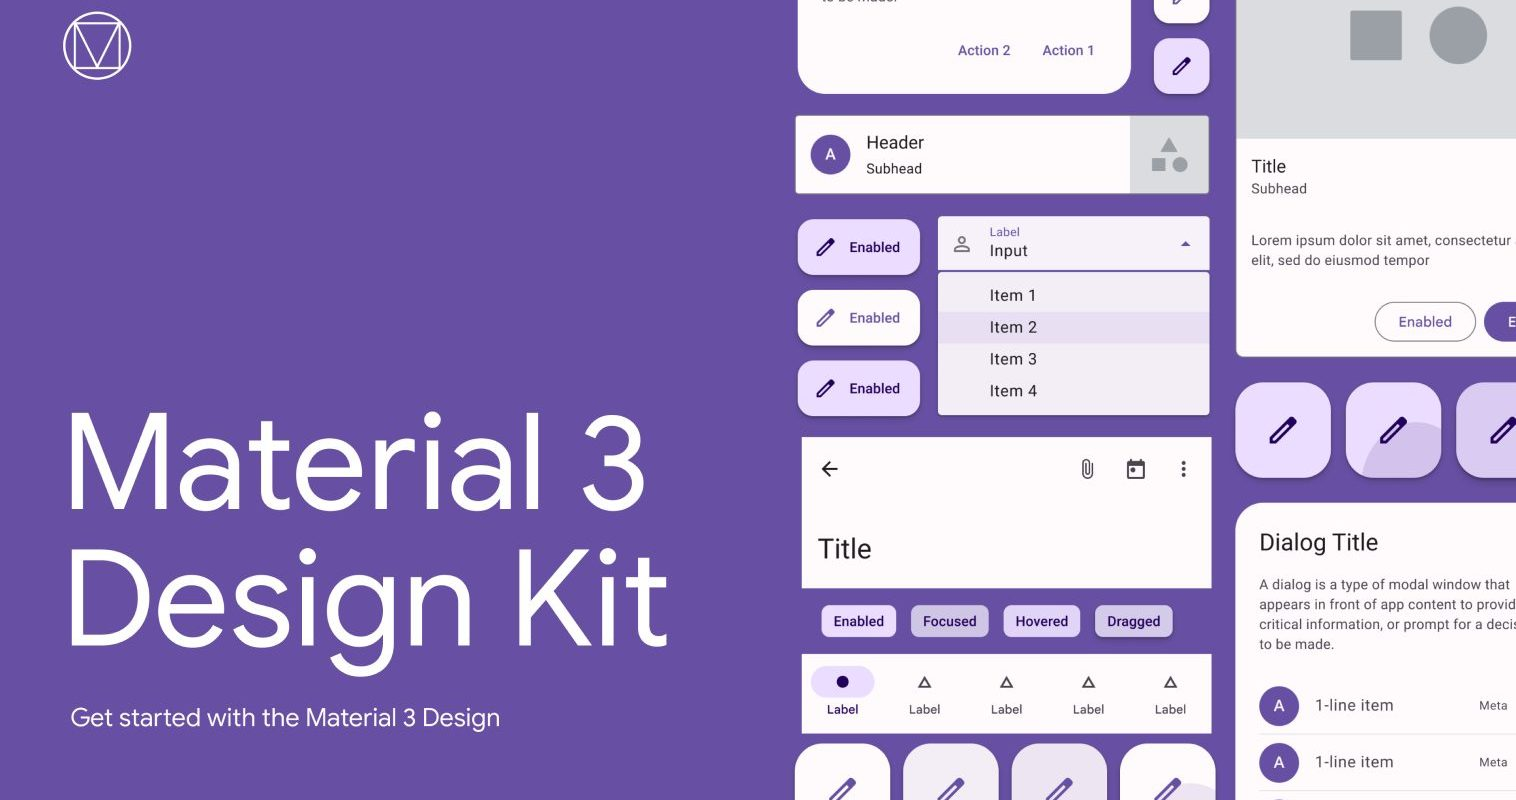
\includegraphics[width=1\textwidth]{Pictures/m3.jpg}
	\caption{Ukázka prvků Material Designu 3 \cite{md3-pic}}
	\label{fig:MD3pic}
\end{figure}

\subsubsection*{noUiSlider}

Drobnou část aplikace tvoří speciální posuvník pro výběr časového okna. Jedná se o~JavaScriptový posuvník noUiSlider. noUiSlider je knihovna pro JavaScript, která umožňuje vytvoření pěkně vypadajících a~snadno ovladatelných posuvníků (sliderů) pro webové stránky. Její posuvníky jsou vysoce přizpůsobitelné: umožňují nastavení více úchytů, poskytují možnost přizpůsobení krokování, dokáží měnit svůj vzhled a~mnoho dalších \cite{nouislider}.

V~naší aplikaci je třeba mít posuvník se dvěma úchyty pro zvolení časového rozmezí od a~do a~přesně tohle noUiSlider umožňuje. Hodnoty posuvníku symbolizují časové okno, které lze rozdělit podle dní, týdnů nebo měsíců.

\subsubsection*{Plotly.js}
\label{plotly}

Mezi poslední využité knihovny patří knihovna Plotly.js. Plotly.js je open-source knihovna pro vytváření interaktivních grafů a~vizualizací na webových stránkách pomocí JavaScriptu. Tato knihovna je vyvinuta společností Plotly, která se specializuje na vizualizaci dat \cite{plotly}. Hlavní schopností této knihovny je vytvářet interaktivní grafy, ať už koláčové, sloupcové, spojnicové nebo bodové. Součástí těchto grafů bývají interaktivní prvky jako přibližování, posouvání nebo řezání grafu na menší části. Velkým bonusem této knihovny je vysoká přizpůsobitelnost. 

Pokud si uživatel v~aplikaci zvolil možnost zobrazovat graf daného okresu, při kliknutí na okres na mapě se objeví interaktivní graf vyobrazujicí vybraná data v~daném okrese. Více o~funkčnosti grafu naleznete v~kapitole \ref{graf}.

\subsubsection*{Google Fonts}

Ačkoli se to nemusí zdát, velkou část aplikace tvoří fonty a~ikony. Aplikace čerpá z~Google Fontů dostupných na \cite{google-fonts}. Společnost Google poskytuje fonty, které jsou zdarma k~použití, a~jejich instalace je velice jednoduchá - pouhé přidání \emph{link} elementu s~odkazem na daný font. Celá aplikace používá font Open Sans, který je k~nahlédnutí na \cite{google-fonts-opensans}. Kromě fontů jsou v~aplikaci hojně používány ikony, které najdete na každém rohu uživatelského prostředí. Tyto ikony jsou taktéž dostupné na stránkách Google Fonts, kde se dají filtrovat podle tvaru, designu nebo tématu. Na těchto stránkách je také možné si ikony přizpůsobit k~vlastnímu použití: je možné nastavit jejich výplň, velikost nebo třeba šířku obrysu.

\subsection{Stažení dat ze serveru}

Aby si mohl uživatel zvizualizovat data v~daném časovém období, je nutné nejprve data stáhnout. Data se stahují z~backendu, kde jsou lokálně uložena v~databázi, takže přístup k~těmto datům je velice rychlý. Jakmile si uživatel zvolí časové okno a~klikne na tlačítko stažení, stáhnou se data pro dané časové období se všemi datasety a~uloží se do paměti. Se serverem se komunikuje pouze při načítání aplikace a~při pokusu o~stažení dat, veškerá vizualizace poté probíhá na straně klienta s~již staženými daty.

\begin{figure}[h]
\centering
\subfloat[Běžné nastavení časového okna]{\label{fig:TimeWindowSettings1}{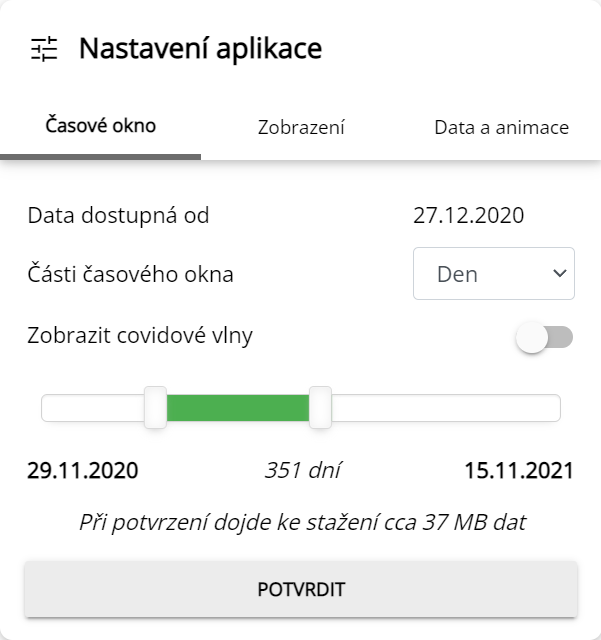
\includegraphics[width=0.4\textwidth]{Pictures/casove_okno1.png}}}\hfill
\subfloat[Zobrazení covidových vln v~posuvníku]{\label{fig:TimeWindowSettings2}
{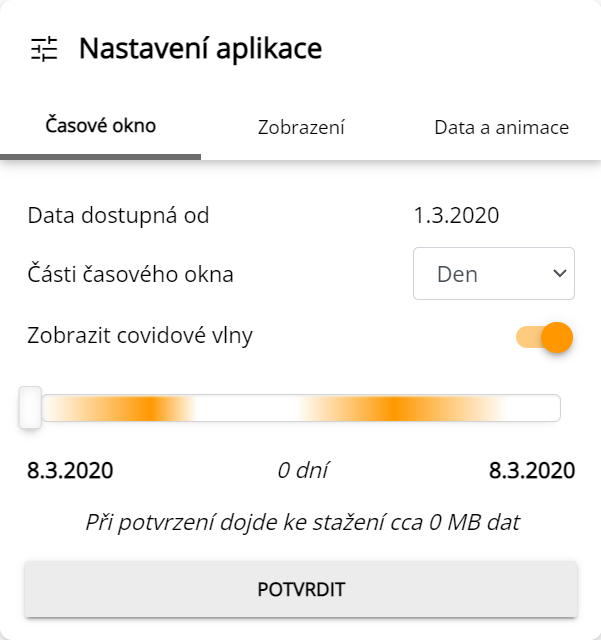
\includegraphics[width=0.4\textwidth]{Pictures/casove_okno2.png}}}
\caption{Nastavení časového okna a~potvrzení stažení dat}
\label{fig:TimeWindowSettings}
\end{figure}

\subsubsection*{Proces stažení dat}

Celý proces stahování začíná kontrolou, zda si již uživatel zvolil dataset k~zobrazení, bez této možnosti by aplikace nevěděla, která data má zobrazit po stažení. Také se zobrazí upozornění v~případě, že má uživatel v~plánu stáhnout více jak 70 \% dostupných dat. Data mohou být v~tomto rozsahu objemná a~jejich stažení může trvat delší dobu. Pokud je objem stažených dat v~pořádku, proběhne výpočet potřebných dní, tzn. že se získají hodnoty zadané v~posuvníku časového okna a~převedou se na potřebný rozsah dní. Z~tohoto rozsahu se vytvoří URL, které bude následně použito k~vytvoření požadavku na backend. Výsledné URL může vypadat takto: \url{http://127.0.0.1:8000/covid/api/from=2021-01-01&to=2023-01-01}. Po vytvoření URL se zašle požadavek na backend, který může buď vrátit data nebo vrátit chybový HTTP kód. Pokud vrátí data, tak se data dekomprimují pomocí knihovny Pako.js a~uloží se do nového slovníku, nastaví se posuvník animace na dané časové rozmezí a~poté se aktualizuje vizualizace společně s~grafem. Pro zjednodušení práce uživatele se také automaticky ukáže záložka s~nastavením animace. Server ale také může vrátit chybový HTTP kód, v~těchto případech je uživatel informován oknem ve spodní části obrazovky (snackbarem), které obsahuje informace o~chybě. Může se jednat buď o~zahlcení serveru uživatelem (příliš časté požadavky), špatný požadavek na backend nebo o~interní chybu na serveru. Možnosti stažení dat lze vidět na obrázcích \ref{fig:TimeWindowSettings}.

\subsection{Vizualizace stažených dat}

Hlavním úkolem této práce je vizualizace dat o~covidu v~okresech ČR. Kapitola \ref{map_creation} popisuje pouhé vytvoření interaktivní mapy, vyobrazení a~využití mapy bude popsáno v~této kapitole. Samotná mapa je vytvořena pomocí knihovny Folium a~je umístěna v~HTML souboru \emph{map.html}.

\subsubsection*{Způsob vyobrazení}

V~hlavním HTML souboru \emph{index.html} se nachází speciální okno, které odkazuje na interaktivní mapu a~zobrazuje ji. Toto okno je realizováno pomocí elementu \emph{iframe}, což je HTML element umožňující vkládání jednoho HTML dokumentu do jiného. Díky použití \emph{iframe} mohou být tyto dvě důležité části aplikace (GUI a~interaktivní mapa) odděleny v~různých HTML souborech. V~Django projektu musí být správně nastaveno \texttt{X\_FRAME\_OPTIONS}, aby \emph{iframe} fungoval správně.

Design tohoto \emph{iframu} byl navržen tak, aby se mapa rozpínala přes celou obrazovku a~GUI \enquote{plavalo} na ní. Mapa se tak stane hlavním prvkem, který uživatel uvidí. Při načítání aplikace ve webovém prohlížeči dojde k~inicializaci mapy. Proběhnou drobné úpravy, které zlepší vzhled mapy a~usnadní práci s~ní. Například dojde k~odstranění neužitečného výběru vrstev mapy (automaticky vygenerováno knihovnou Folium), okresům na obrysu ČR se přiřadí identifikační čísla a~názvy pro snazší manipulaci a~také se nastaví okno, které se má zobrazit při kliknutí myší na okres.  

Po načtení hlavní stránky se zobrazí GUI s~mapou soustředěnou na střední Evropu, která se skládá z~dlaždic (tilů) poskytovaných OpenStreetMap. Tyto dlaždice se postupně načítají při posunu nebo přibližování a~oddalování mapy. Na této mapě se pomocí elementu \emph{svg} zobrazí obrys České republiky rozdělený na okresy, kde každý okres má bílou barvu s~lehkou průhledností. Tento obrys ČR se pohybuje s~mapou světa při posunu nebo přibližování díky skriptům knihovny Leaflet, která je součástí mapy.

Uživatel brzy po načtení stránky zjistí, že nám tato mapa neposkytuje žádné covidové informace. Vše se změní, jakmile uživatel zvolí dataset, časové okno a~potvrdí svou volbu. Pokud byla volba platná, spustí se hlavní funkce \lstinline{updateMap}, tato funkce se také volá vždy, když uživatel změní hodnotu posuvníku v~záložce nastavení \emph{Data a~animace}. Tento posuvník reprezentuje počet dní ve zvoleném časovém okně. Funkce \lstinline{updateMap} začíná tím, že získá aktuální datum ze zmíněného posuvníku, které má zobrazit. Poté se zkontroluje, zda daný dataset obsahuje informace o~vybraném dni. Pokud ne, zobrazí se upozornění (viz. obrázek \ref{fig:WarningMap}). V~opačném případě funkce pokračuje a~získá si potřebná data.

\begin{figure}[h]
	\centering
	
\includegraphics[width=0.8\textwidth]{Pictures/warning.png}
	\caption{Upozornění absence dat v~datasetu}
	\label{fig:WarningMap}
\end{figure}

Aby aplikace věděla která data má hledat, existuje externí slovník v~souboru \emph{data\_analysis\_types.js}, který si aplikace načte při startu. Tento slovník obsahuje klíče, které má aplikace hledat ve stažených datech podle zvoleného datasetu. Zkontroluje se, zda se aplikují nějaké přepočty nebo zda se škálují barvy vůči nejvyšší nalezené hodnotě v~daném časovém okně. Po těchto přípravách funkce prochází všechny okresy ČR na mapě a~vypočítá pro každý okres jeho výslednou barvu na mapě. Tato barva se určuje podle datasetu (zelená, fialová, šedá a~oranžová) a~podle nalezené hodnoty ve stažených datech pro daný den (výrazná nebo málo výrazná). Mimo jiné se také aktualizuje barevná škála a~informační text o~datasetu v~levém spodním okně aplikace. Dále se aktualizuje okno s~informacemi o~okrese, pokud uživatel klikne na nějaký okres tlačítkem myši.

Výsledkem je plnohodnotná mapa, která barevně vyobrazuje zvolená data v~konkrétní den a~automaticky se aktualizuje při změně datasetu, časového okna nebo dne. Mapa také obsahuje interaktivní prvky, například při najetí myši na okres se zobrazí jeho název pro lepší orientaci a~po kliknutí na okres se zobrazí jeho přesné hodnoty. Výslednou mapu lze vidět na obrázku \ref{fig:MapExample}.

\begin{figure}[h]
	\centering
	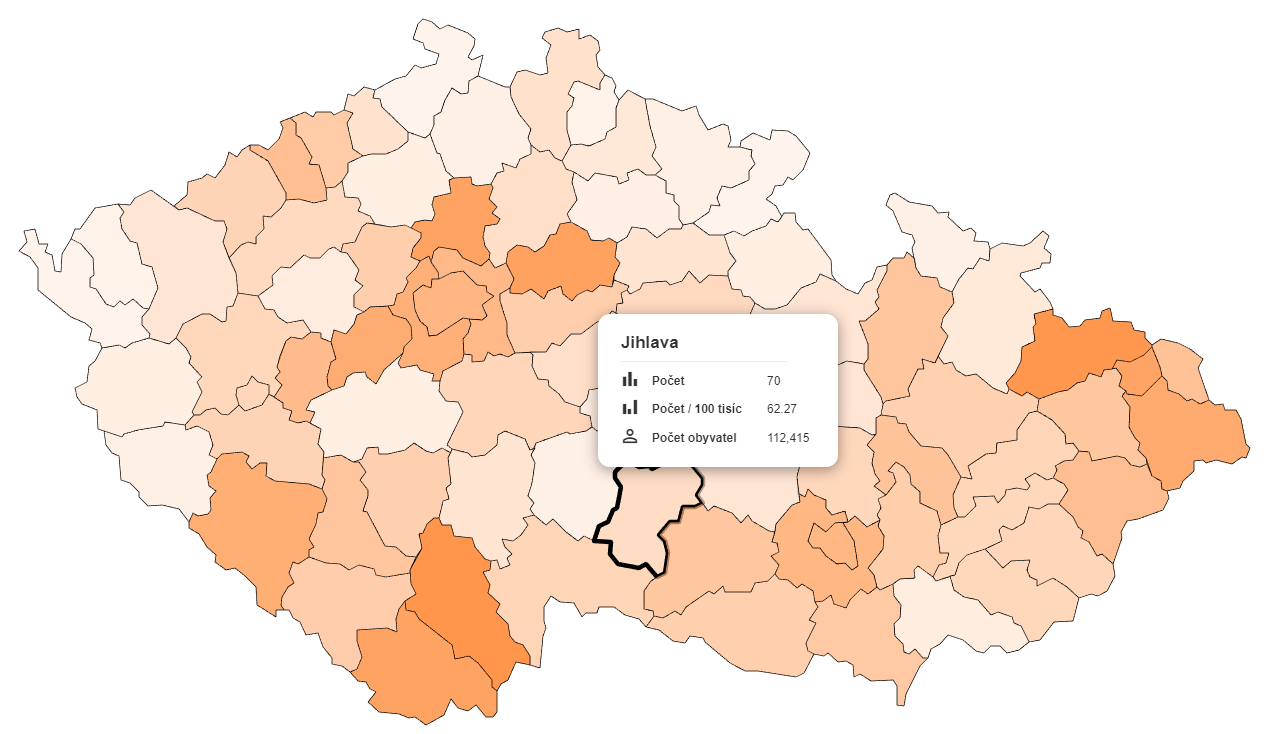
\includegraphics[width=0.8\textwidth]{Pictures/mapa.png}
	\caption{Příklad výsledné mapy infekcí s~otevřeným pop-up oknem}
	\label{fig:MapExample}
\end{figure}

\subsection{Přizpůsobení vizualizace}

Jakmile si uživatel zvolí dataset a~stáhne data, automaticky se zobrazí covidové informace na mapě od prvního dne ve zvoleném časovém okně. V~původním stavu jsou veškeré hodnoty zobrazeny s~přepočtem na 100 tisíc obyvatel. Díky tomu můžeme lépe spatřit rozdíly v~různých okresech vzhledem k~přesnějšímu porovnání. Takové hodnoty ale nemusí uživateli stačit a~proto aplikace poskytuje širokou škálu nastavení časového období a~hodnot.

Mapa podporuje základní funkce jako například přibližování, oddalování a~posouvání. Ovládat přiblížení mapy se dá několika způsoby. Pravděpodobně nejčastější způsob je posouvání kolečkem na myši, lze ale také přibližovat dvojklikem na mapu nebo pomocí kláves na klávesnici + a~-. Posouvat mapu lze dotykem, pokud máte dotykovou obrazovku, ale také standartně přidržením levého tlačítka myši a~posunutím. Podobně jako u~přiblížení lze mapu posouvat pomocí šipkových kláves.

\subsubsection*{Škálování hodnot}

Jak bylo zmíněno, v~původním stavu jsou hodnoty automaticky přepočteny na 100 tisíc obyvatel v~daném okrese. Kvůli tomu je třeba znát počty obyvatel v~okresech, to ale není problém díky datům z~ČSÚ (viz. kapitola \ref{csu}). Tyto přepočty vyobrazují covidovou situaci přesněji neboť bez tohoto přepočtu by mohly být vyobrazené hodnoty zkreslené. Představme si počty nakažených, pravděpodobně budou tyto počty neustále velké ve městech, kde je vysoká populace. Může se ale stát, že v~dané vesnici nejsou tyto počty nakažených tak vysoké, jako ve městech, ale v~poměru s~neinfikovanými mohou představovat značnou část. Proto existuje přepočet na daný počet obyvatel, který lépe zachycuje reálnou situaci v~místě. Uživateli je umožněno tento přepočet ovládat a~může si jej podle svého uvážení vypnout nebo zapnout.

K~dispozici je také škálování barev podle maximální nalezené hodnoty v~časovém okně. V~původním nastavení je tato možnost vypnuta a~místo toho se barvy na mapě škálují podle největší nalezené hodnoty v~daný den. Toto nastavení dokáže lépe zvýraznit průběh tzv. covidových vln. Pokud si uživatel stáhne všechna dostupná data, tak při zapnutém škálování podle maximální nalezené hodnoty spatří několik období, kdy covid-19 nejvíce postihl Českou republiku.

Je důležité zmínit, že veškerá tato nastavení škálování se aplikují i~na minimapu v~obraze v~obraze. Z~technického hlediska se při změně škálování hodnot neděje nic zásadního, při změně přepínačů reprezentujících tato škálování dojde ke změně proměnné, která se kontroluje ve funkci \lstinline{updateMap}. Tyto proměnné definují, zda jsou tato škálování aktivní nebo ne. Také dojde k~okamžitému zavolání funkce \lstinline{updateMap}, aby se aktualizovaly aktuálně zobrazované hodnoty.

\begin{figure}[h]
	\centering
	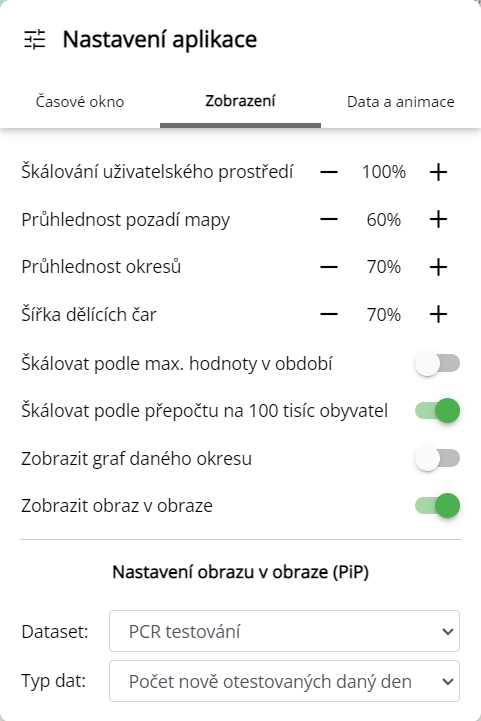
\includegraphics[width=0.5\textwidth]{Pictures/nastaveni.png}
	\caption{Dostupné nastavení mapy a~škálování}
	\label{fig:AppSettings}
\end{figure}

\subsubsection*{Grafické přizpůsobení mapy}

Uživateli je umožněno si mapu graficky přizpůsobit v~nastavení aplikace v~záložce \emph{Zobrazení}. Každý uživatel může interaktivní mapu využít jiným způsobem, některý uživatel může chtít vidět pouze obrys ČR, někteří uživatelé možná chtějí vidět podklad mapy v~okresech. K~dispozici je široká škála přizpůsobení. Nastavení zobrazení lze vidět na obrázku \ref{fig:AppSettings}.

Přizpůsobit lze průhlednost mapy, která slouží jako podklad k~okresům ČR. V~původním stavu je nastavena na 60 \%, lze ji ale měnit v~krocích po 10 \% od 0 \% až do 100 \%. Ve výsledku můžeme mapu zcela skrýt nebo ji nechat plně viditelnou.

Mimo mapu lze měnit i~styl okresů v~obrysu ČR. Podobně jako u~mapy lze měnit jejich průhlednost a~tím zvýraznit nebo zeslabit jejich barevnou hodnotu. Díky tomu lze okresy zcela skrýt, pokud je to potřeba, nebo je naopak zvýraznit, protože jejich původní průhlednost je nastavena na 70 \%.

Co se týče grafického přizpůsobení mapy, tak lze také měnit tloušťku dělicích čar mezi okresy. Lze tak kompletně skrýt hranice okresů nebo naopak je zvýraznit. Původní tloušťka je nastavena na 70 \%.

Všechna tato nastavení mění styl buď samotné mapy nebo okresů. Pro změnu průhlednosti se mění vlastnost \texttt{opacity} nebo \texttt{fill-opacity} a~pro změnu šířky hran okresů se mění \texttt{stroke-width}. 

\subsubsection*{Animace}

Je důležité zmínit schopnost aplikace animovat data. Jedná se o~velice důležitou část, díky které se aplikace stává mnohem zajímavější, neboť uživatel samotný se stává režisérem své animace. Animovat data v~tomto případě znamená postupně vyobrazovat dny časového okna za sebou. Rychlost změny dní se dá upravit, aplikace poskytuje rychlosti od jedné do deseti, kde se jedná o~pomalou rychlost po nejvyšší. Díky této schopnosti animovat data lze pozorovat různé úkazy v~datech, například sledovat šíření koronaviru a~zpozorovat tak covidové vlny nebo lze také sledovat šíření infekce z~různých světových stran.

\begin{figure}[h]
	\centering
	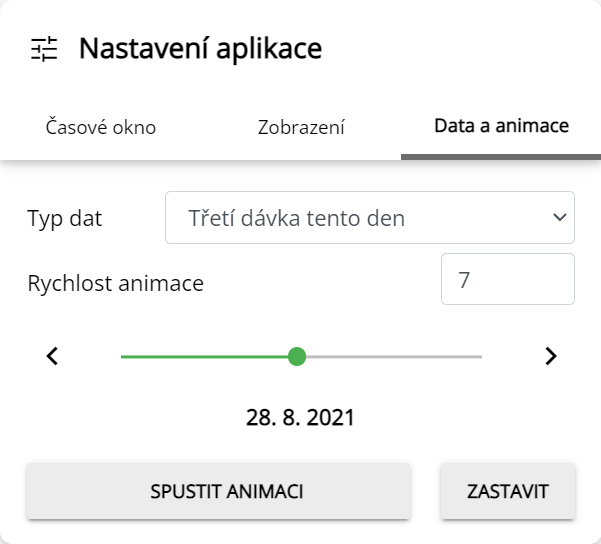
\includegraphics[width=0.5\textwidth]{Pictures/animace.png}
	\caption{Volba typu dat a~nastavení animace}
	\label{fig:AnimationSettings}
\end{figure}

Ovládání animace se nachází v~nastavení aplikace v~záložce \emph{Data a~animace}, kde se nachází posuvník dní i~přepínač rychlosti. Uživatel může pomocí tlačítka \emph{Zastavit} kdykoli animaci vypnout a~pozastavit se v~posledním přehrávaném dni.

\subsubsection*{Výběr dat z~datasetu}

V~záložce \emph{Data a~animace} je na výběr z~několik typů dat. Tato data korespondují s~vybraným datasetem a~lze je libovolně měnit i~v~průběhu animace. Každý dataset poskytuje alespoň dva typy dat, často se jedná o~hodnoty reprezentující přírůstky daný den a~poté celkové hodnoty od sbírání dat po daný den. Některé datasety obsahují více typů dat, například očkování poskytuje informace o~každé dávce zvlášť. Výsledné okno s~volbou typu dat je na obrázku \ref{fig:AnimationSettings}.

\subsection{Obraz v~obraze}
\label{pip}

S~funkcí obraz v~obraze se pravděpodobně setkáte v~televizích obrazovkách. Jedná se o~schopnost zobrazit současně dva obrazy různých televizních stanic nebo jiných zdrojů (např. DVD přehrávač nebo herní konzole). Aplikace se touto funkcí inspirovala a~obsahuje podobnou funkci. V~tomto případě se jedná o~zobrazení dvou různých typů dat zároveň. K~realizaci je potřeba druhá mapa, nebo alespoň obrys ČR, která bude uživateli viditelná. Aplikace takovou mapu obsahuje, ale není v~původním stavu viditelná. Pro její aktivaci je nutné použít přepínač v~nastavení aplikace v~záložce \emph{Zobrazení}. Jakmile se přepínač aktivuje, zobrazí se v~pravém horním rohu obrazovky minimapa, která bude zobrazovat vybraná data.

\begin{figure}[h]
	\centering
	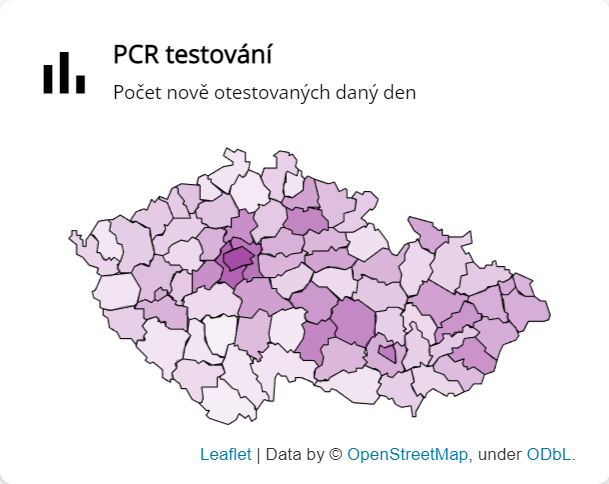
\includegraphics[width=0.5\textwidth]{Pictures/pip.png}
	\caption{Obraz v~obraze}
	\label{fig:PictureInPicture}
\end{figure}

Tato minimapa funguje na stejném principu jako hlavní mapa. Při načtení aplikace se inicializuje podobně jako hlavní mapa a~její aktualizace probíhá ve stejné funkci \lstinline{updateMap}. S~mapou ale nelze nijak manipulovat a~nereaguje na pohyby a~stisky myší nebo klávesnice. Po sepnutí přepínače se okno s~nastavením aplikace rozšíří o~nové prvky - výběry datasetu a~typu dat z~datasetu. Okno s~minimapou se automaticky aktualizuje při výběru nového typu dat.

Obraz v~obraze má mnoho využití, je možné porovnávat v~jeden okamžik přírůstky a~celkové hodnoty nebo třeba hledat souvislosti mezi dvěma datasety. Ukázkové použití obrazu v~obraze lze spatřit v~obrázku \ref{fig:PictureInPicture}.



\subsection{Graf}

Graf společně s~obrazem v~obraze jsou jediné části aplikace, které se v~původním stavu nezobrazují. Je třeba jej zapnout v~nastavení aplikace v~záložce \emph{Zobrazení}. Vygenerovaný graf je výsledkem knihovny Plotly.js. Více informací o~této knihovně je v~kapitole \ref{plotly}.

Graf vyobrazuje zvolený typ dat pro daný okres. Aby si uživatel zvolil okres, musí na okres myší kliknout. Po kliknutí se volá funkce \lstinline{initChart}, která inicializuje graf pro daný okres. Nejprve si funkce zjistí časové okno a~pro každé datum z~časového okna si zajistí příslušné hodnoty. Tyto hodnoty získává ze stažených dat a~vybere si pouze ta data, se kterými uživatel právě pracuje. Jakmile data získá, dojde k~definování vzhledu grafu (nastavení titulku, barev atd.). Na závěr se zavolá funkce knihovny Plotly.js \lstinline{newPlot}, které se předávají konfigurace a~také ID elementu, kde se má nově vytvořený graf zobrazit.

Výsledkem tohoto procesu je interaktivní graf zobrazující aktuálně zkoumananá data. Součástí grafu jsou i~popisky, které obsahují název právě zvoleného okresu a~rozsah časového okna. Knihovna Plotly.js do grafu automaticky přidá interaktivní prvky, díky kterým získává graf více možností. Je možné se v~grafu libovolně pohybovat a~také je možné jej přiblížit nebo oddálit. Zajímavou funkcí je možnost \enquote{rozsekat} si graf na menší části a~zkoumat tyto části dopodrobna. V~grafu je uživateli umožněno zobrazit pomocné čáry nebo třeba vytvořit snímek grafu, který lze uložit lokálně do zařízení.

\begin{figure}[h]
	\centering
	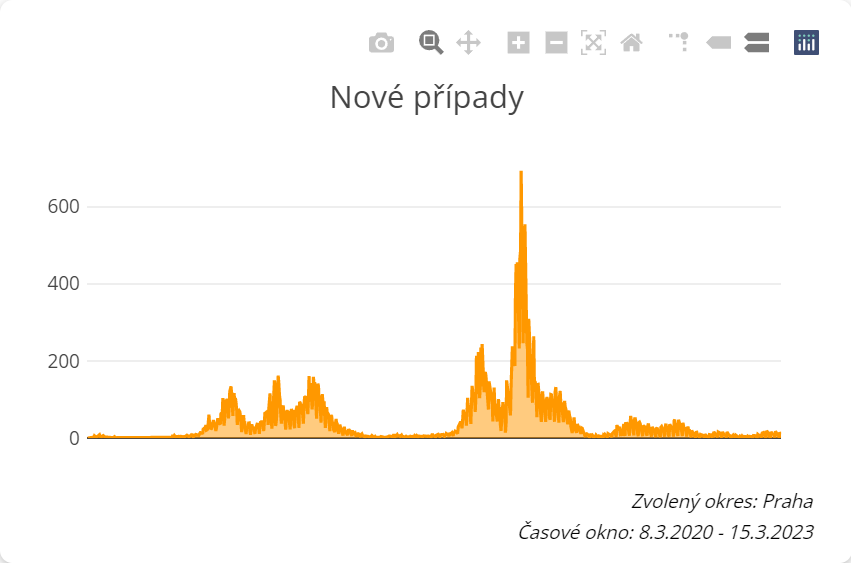
\includegraphics[width=0.5\textwidth]{Pictures/graf.png}
	\caption{Graf v~aplikaci}
	\label{fig:GrafApp}
\end{figure}

\label{graf}

Je nutné podotknout, že okno s grafem nereaguje na změny škálování GUI. Knihovna Plotly.js na toto škálování nereaguje vhodně a dochází k různým grafickým chybám v grafu. Proto si graf zachovává stejnou velikost při změnách škálování GUI. 

\subsection{Tmavý režim}

Drobnou součástí aplikace je tmavý režim, který si může uživatel aktivovat. Po analýze výsledné webové stránky se došlo k~takovému závěru, že je webová stránka příliš světlá a~nemusí dobře působit na oči uživatele. Nejvíce se tento problém vyskytuje při nastavení průhlednosti pozadí mapy na nízkou hodnotu neboť poté obsahuje mapa téměř čistě bílé pozadí. Proto byl v~aplikaci zaveden tmavý režim, který tento problém řeší. Přepínač tmavého režimu se nachází v~pravé horní části obrazovky. Tmavý režim aplikuje tmavou barvu na pozadí a~světlou barvu na popředí veškerých světlých elementů webové stránky. Nastavení temného režimu si bude prohlížeč při dalším přístupu k~aplikaci pamatovat díky uložení hodnoty do lokálního úložiště prohlížeče. Porovnání světlého a~tmavého režimu lze vidět na skupině obrázků \ref{fig:WhiteDarkMode}.
\vspace*{0.5in}
\begin{figure}[h]
\centering
\subfloat[Světlý režim]{\label{fig:WhiteMode}{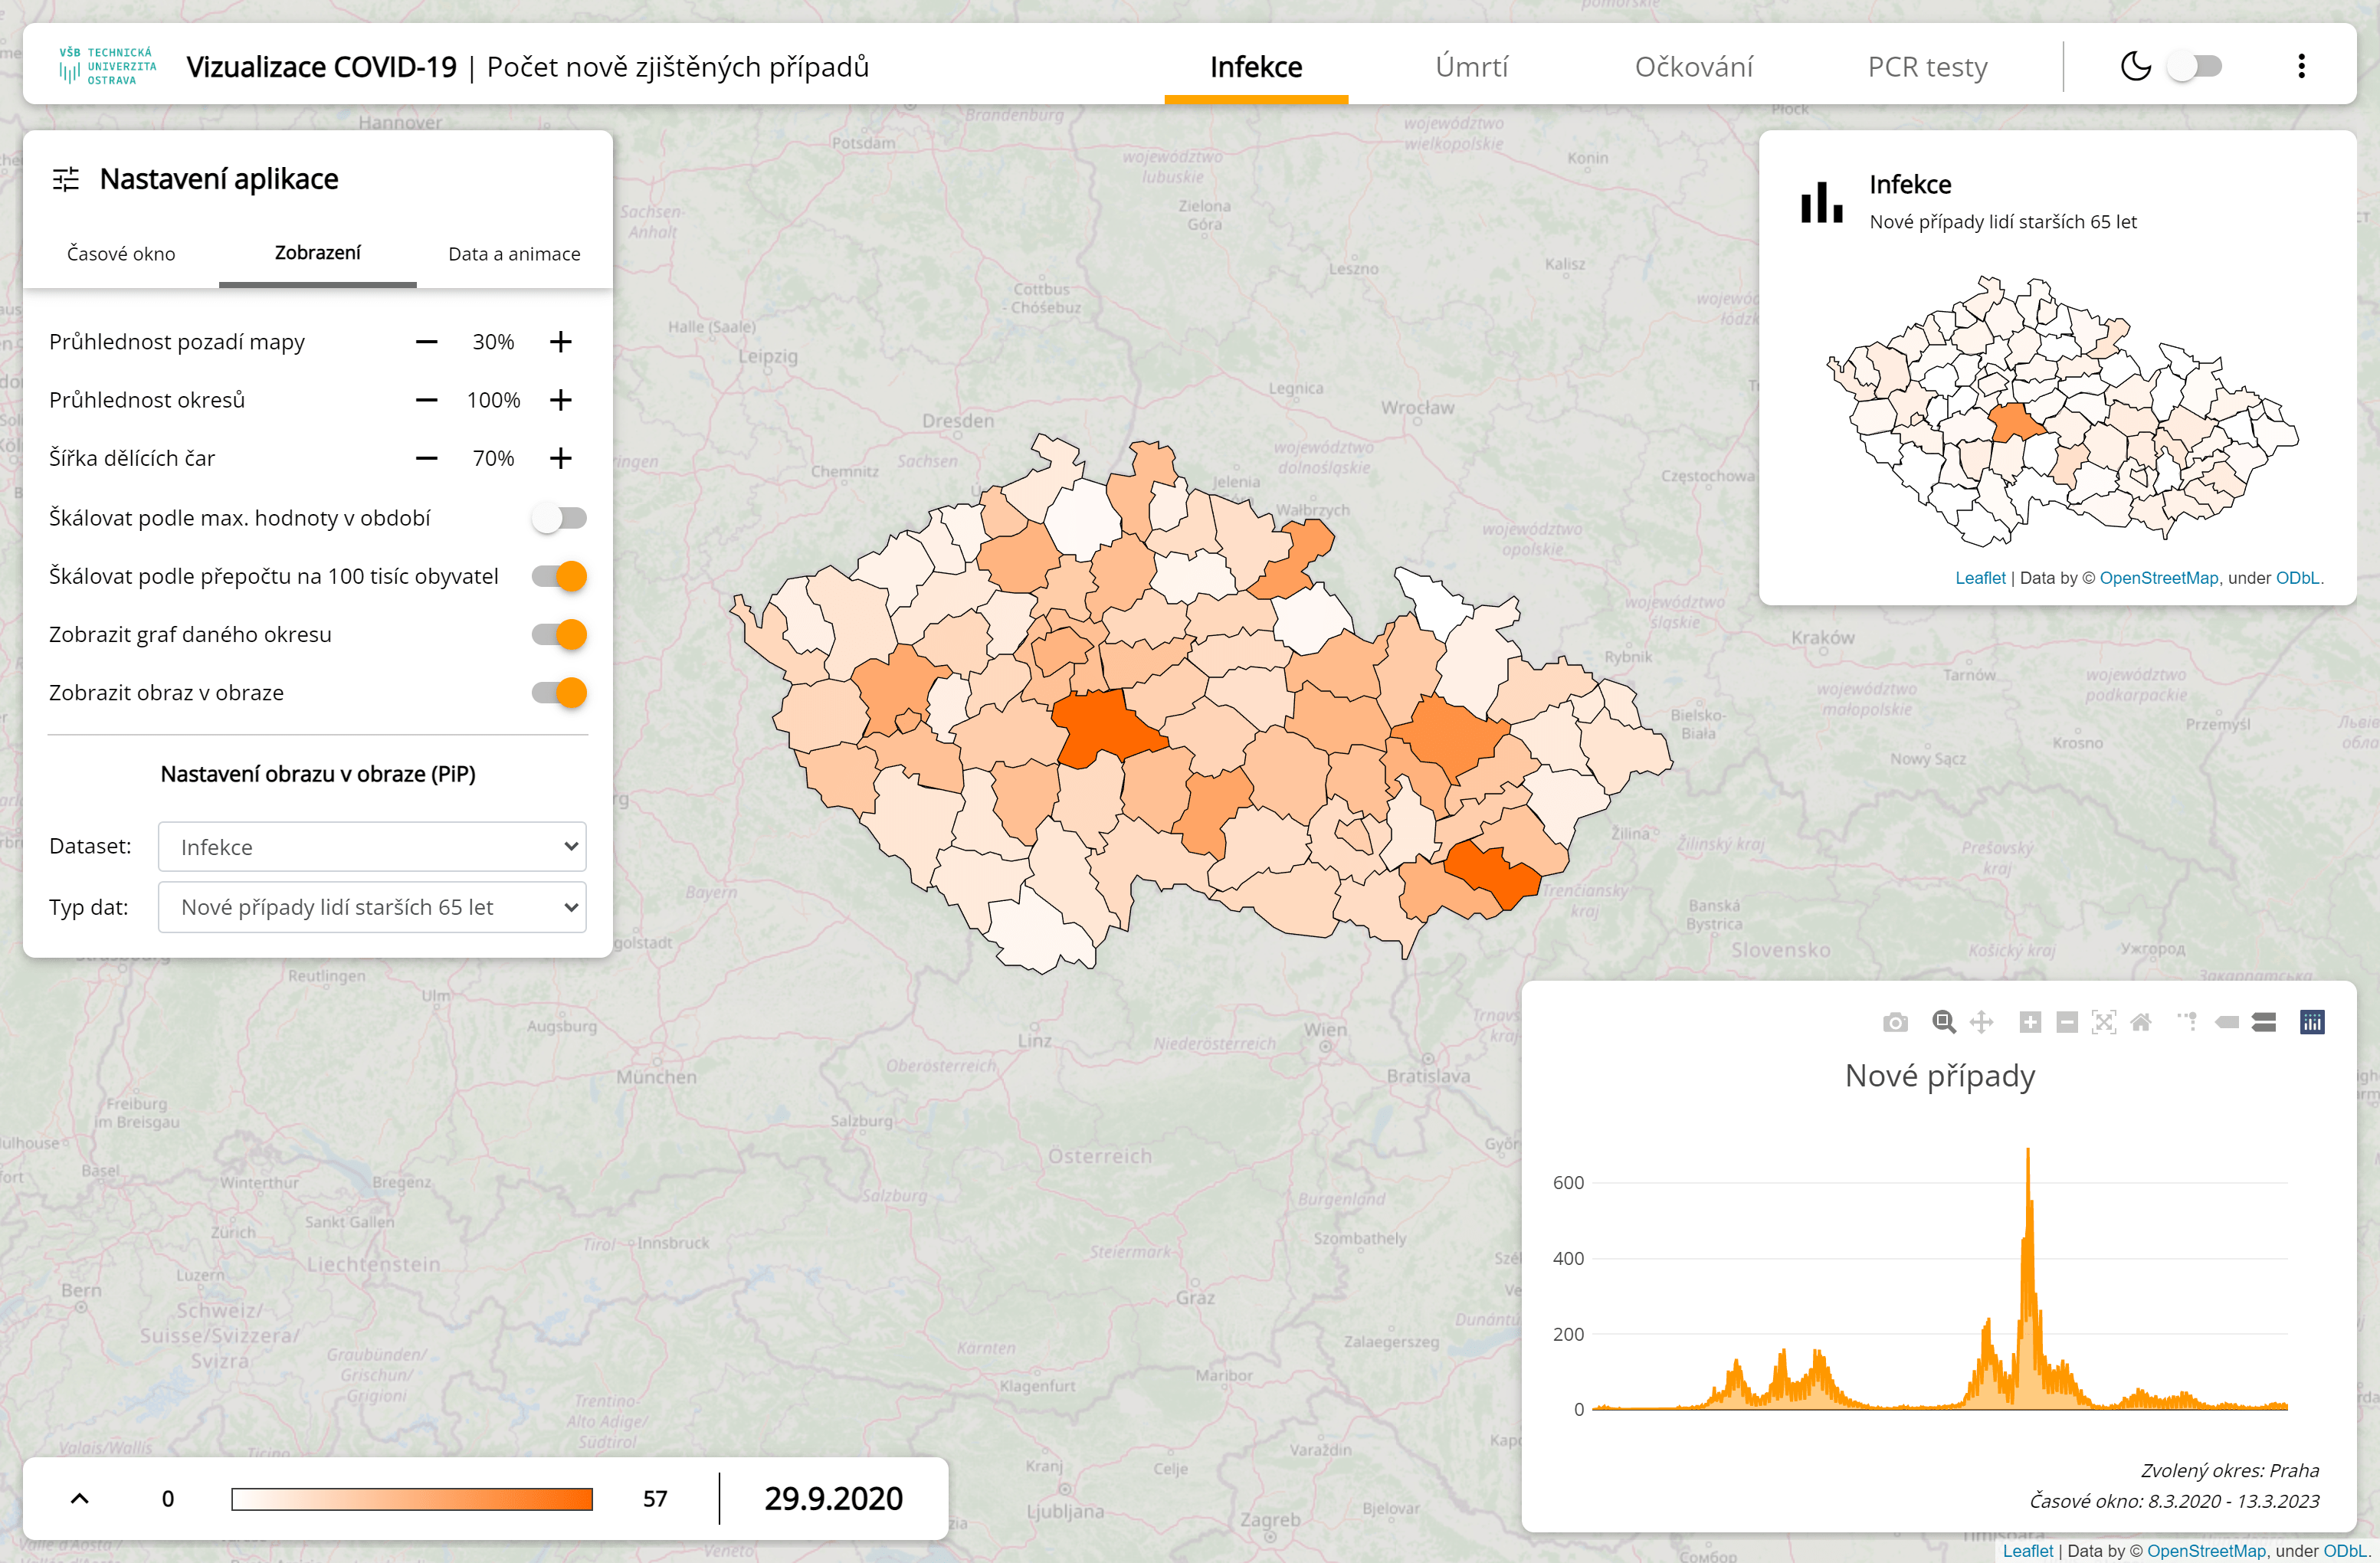
\includegraphics[width=0.85\textwidth]{Pictures/map_white.png}}}\hfill
\subfloat[Tmavý režim]{\label{fig:DarkMode}
{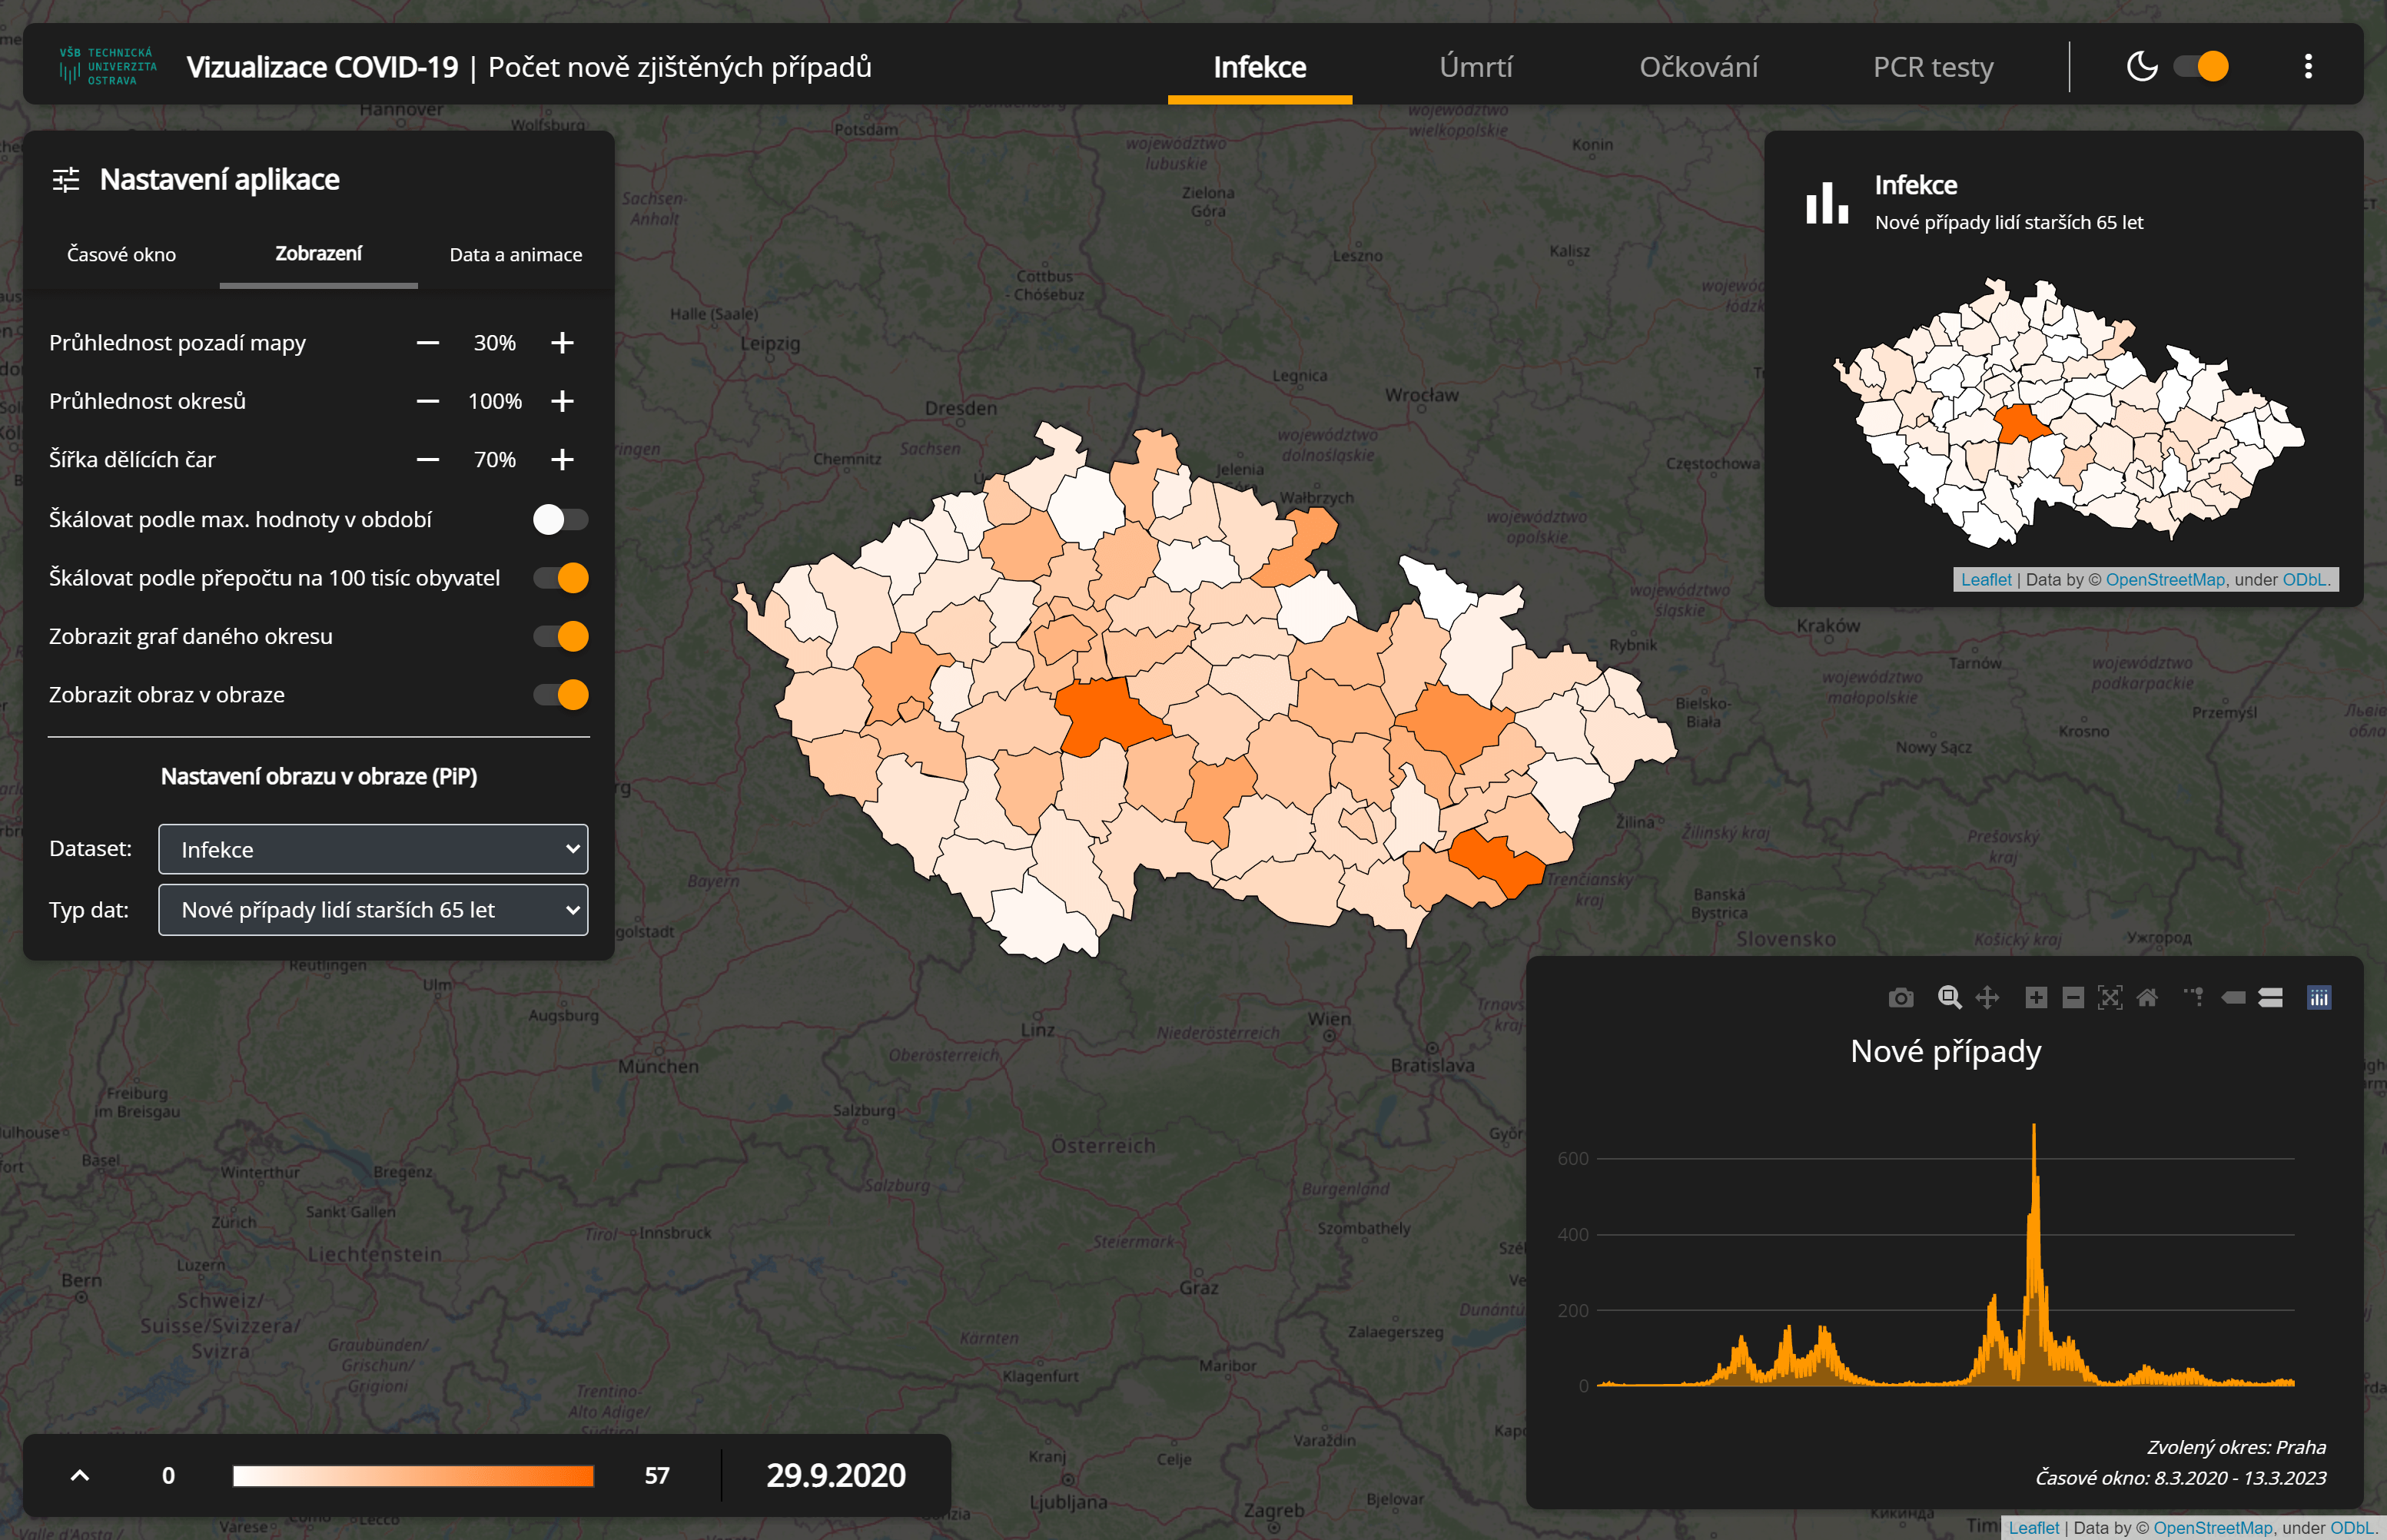
\includegraphics[width=0.85\textwidth]{Pictures/map_dark.png}}}
\caption{Porovnání světlého a~tmavého režimu}
\label{fig:WhiteDarkMode}

\end{figure}

\clearpage

\section{Ukázky využití a~testování výsledné aplikace}

\subsubsection*{Pozorování vybraného dne a~okresu}

Klasickým využití aplikace může být pozorování zvoleného dne a~okresu. Na posuvníku časového okna je možné vybrat jediný den (nebo i~týden či měsíc). Následně stačí kliknout na vybraný okres a~pozorovat změny při přepínání datasetů. Na skupině obrázků \ref{showcase5} lze spatřit okres Jihlava (a~zbytek ČR) ve všech čtyřech datasetech. Na prvním obrázku jsou nové přírůstky nakažených, na druhém nová vydaná očkování jakékoli dávky, na třetím jsou zaznamenaná úmrtí a~na čtvrtém obrázku je znázorněný počet provedených PCR testů. Zvolený den je 4. dubna 2022.

\vspace*{0.5in}
\begin{figure}[h]
\centering
\begin{tabular}{cc}
  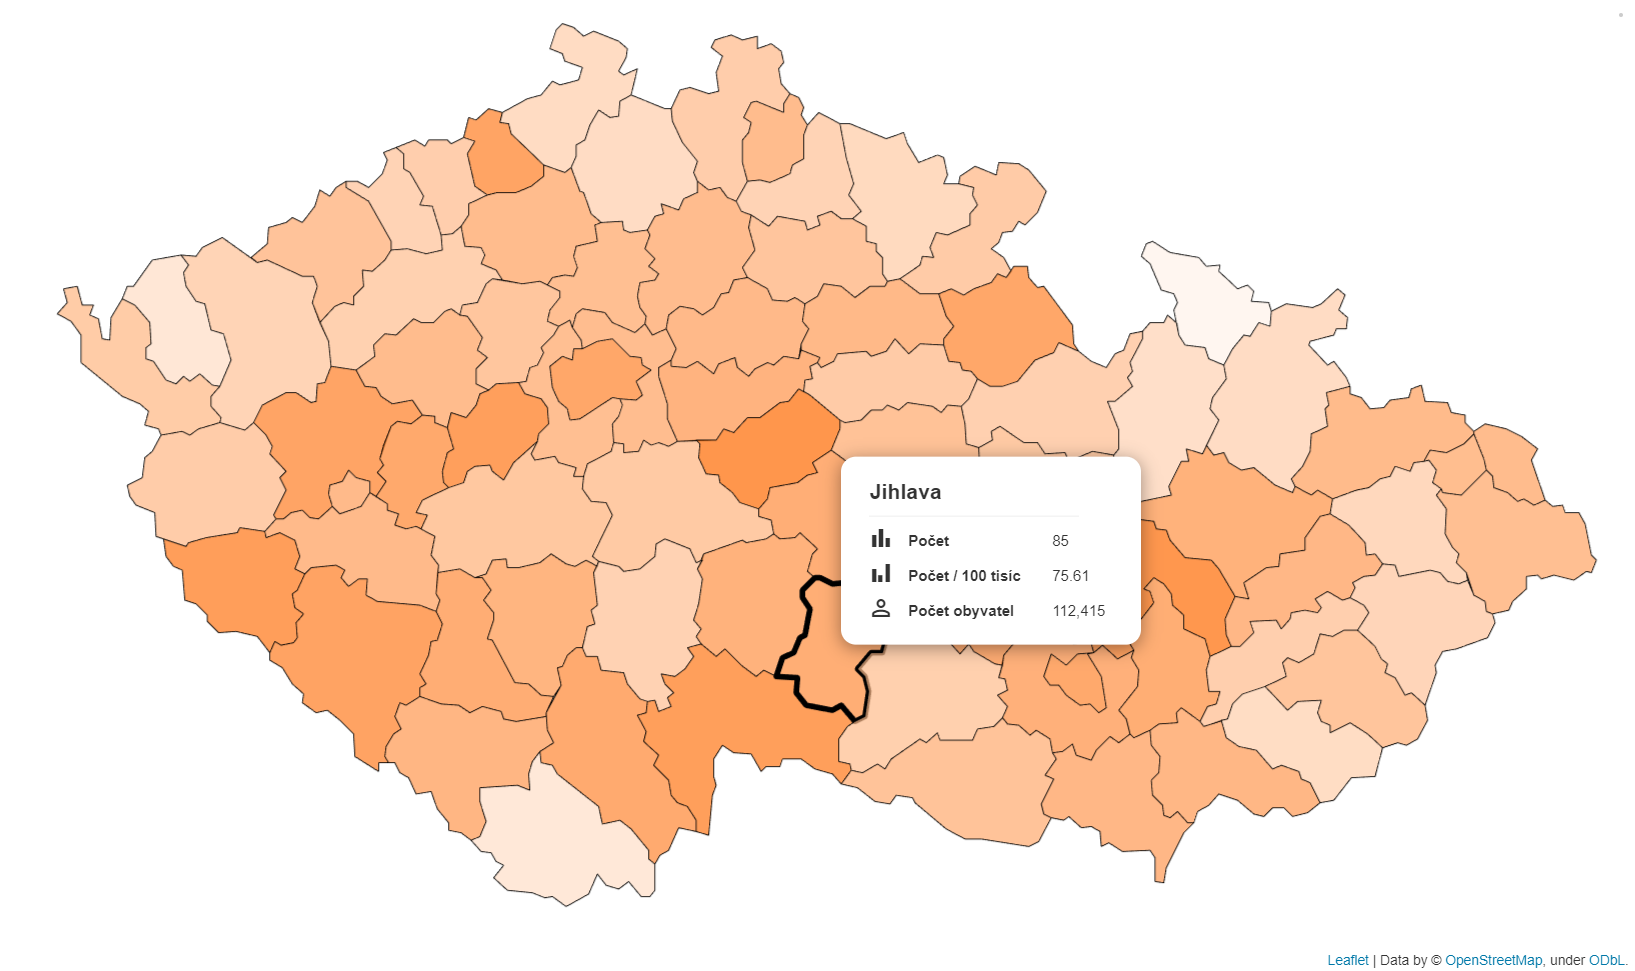
\includegraphics[width=0.47\textwidth]{Pictures/showcase5a.png} &   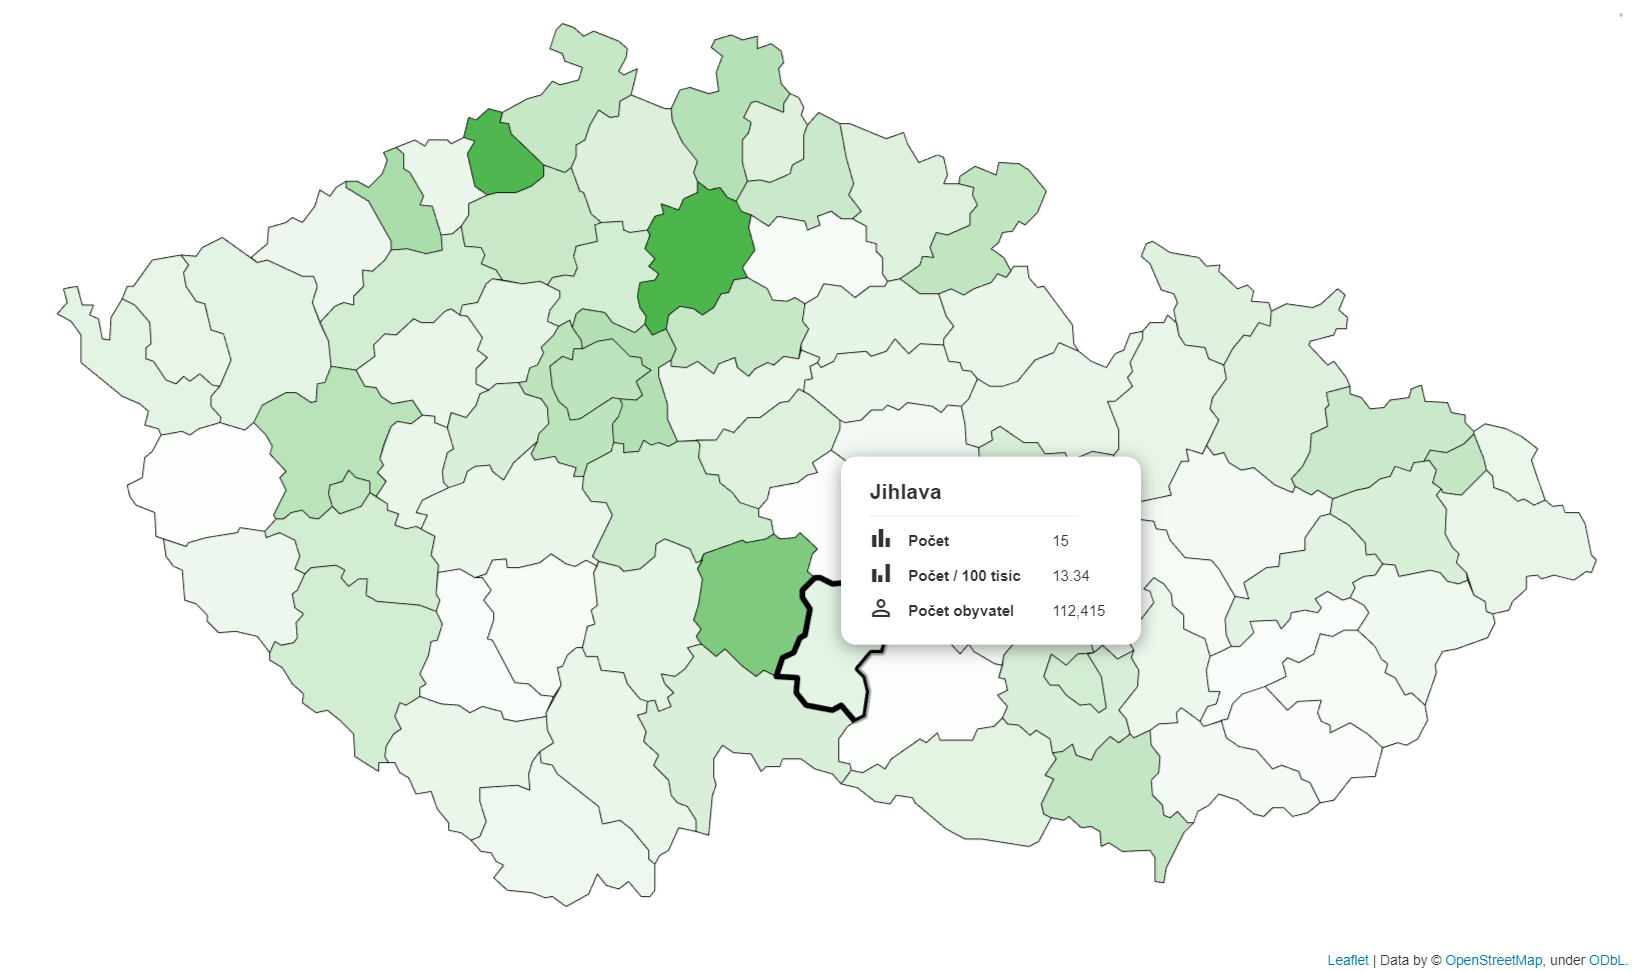
\includegraphics[width=0.47\textwidth]{Pictures/showcase5b.png} \\
(a) Nové případy infekce & (b) Vydané dávky očkování \\[6pt]
\\
\\
\\
 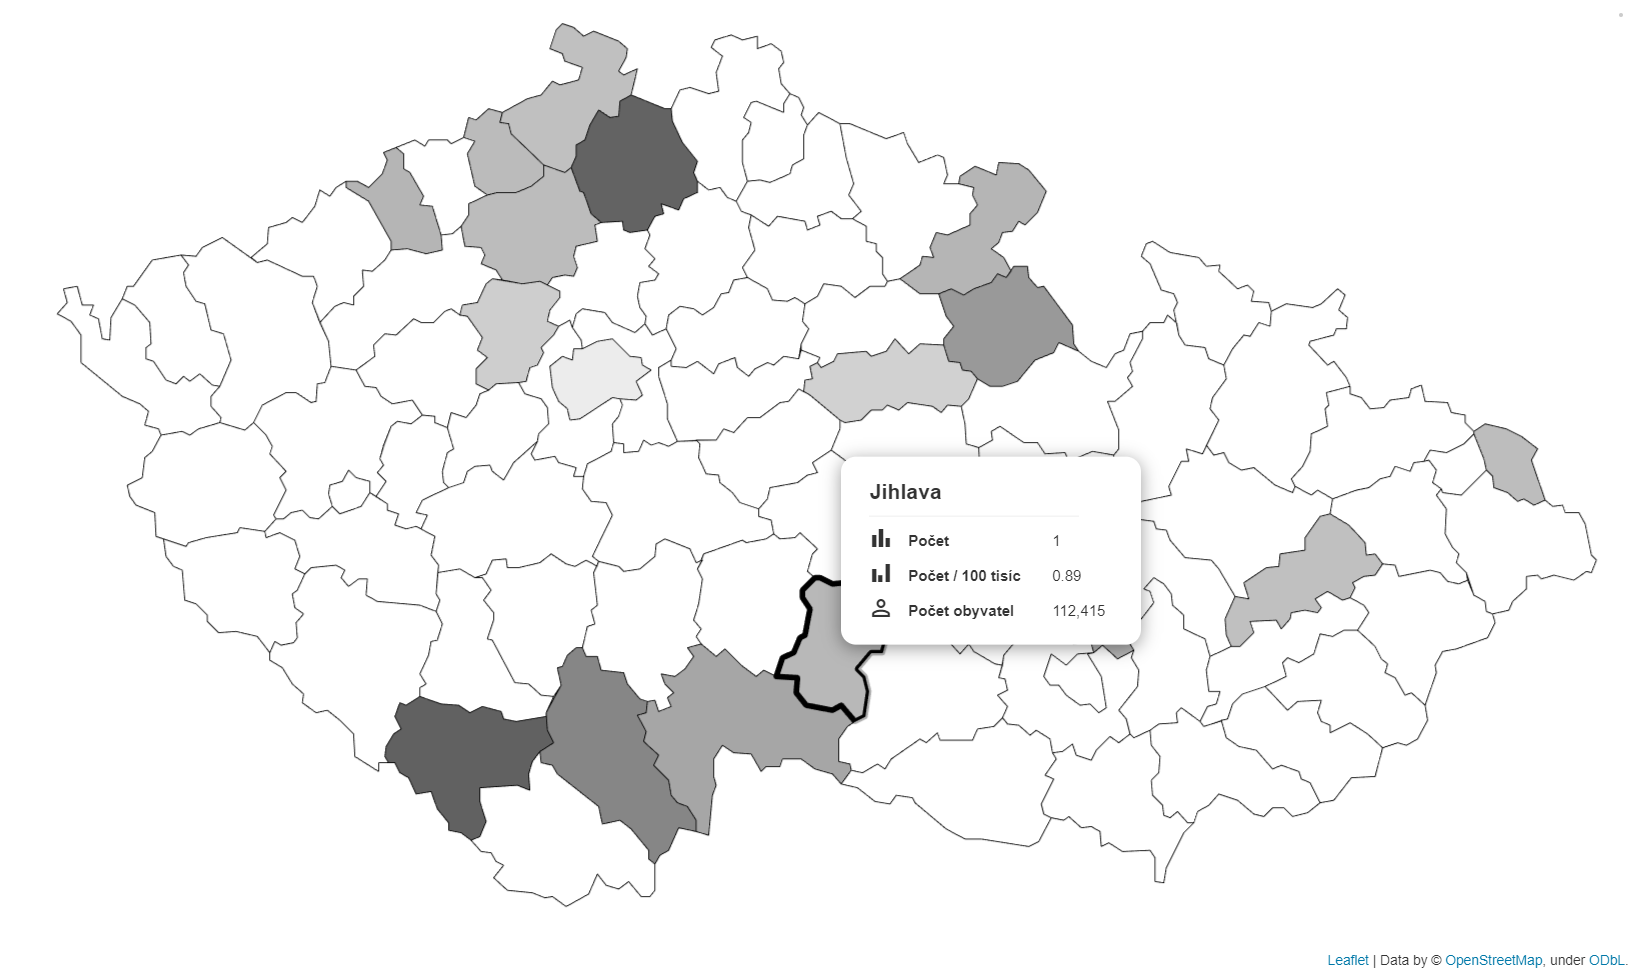
\includegraphics[width=0.47\textwidth]{Pictures/showcase5c.png} &   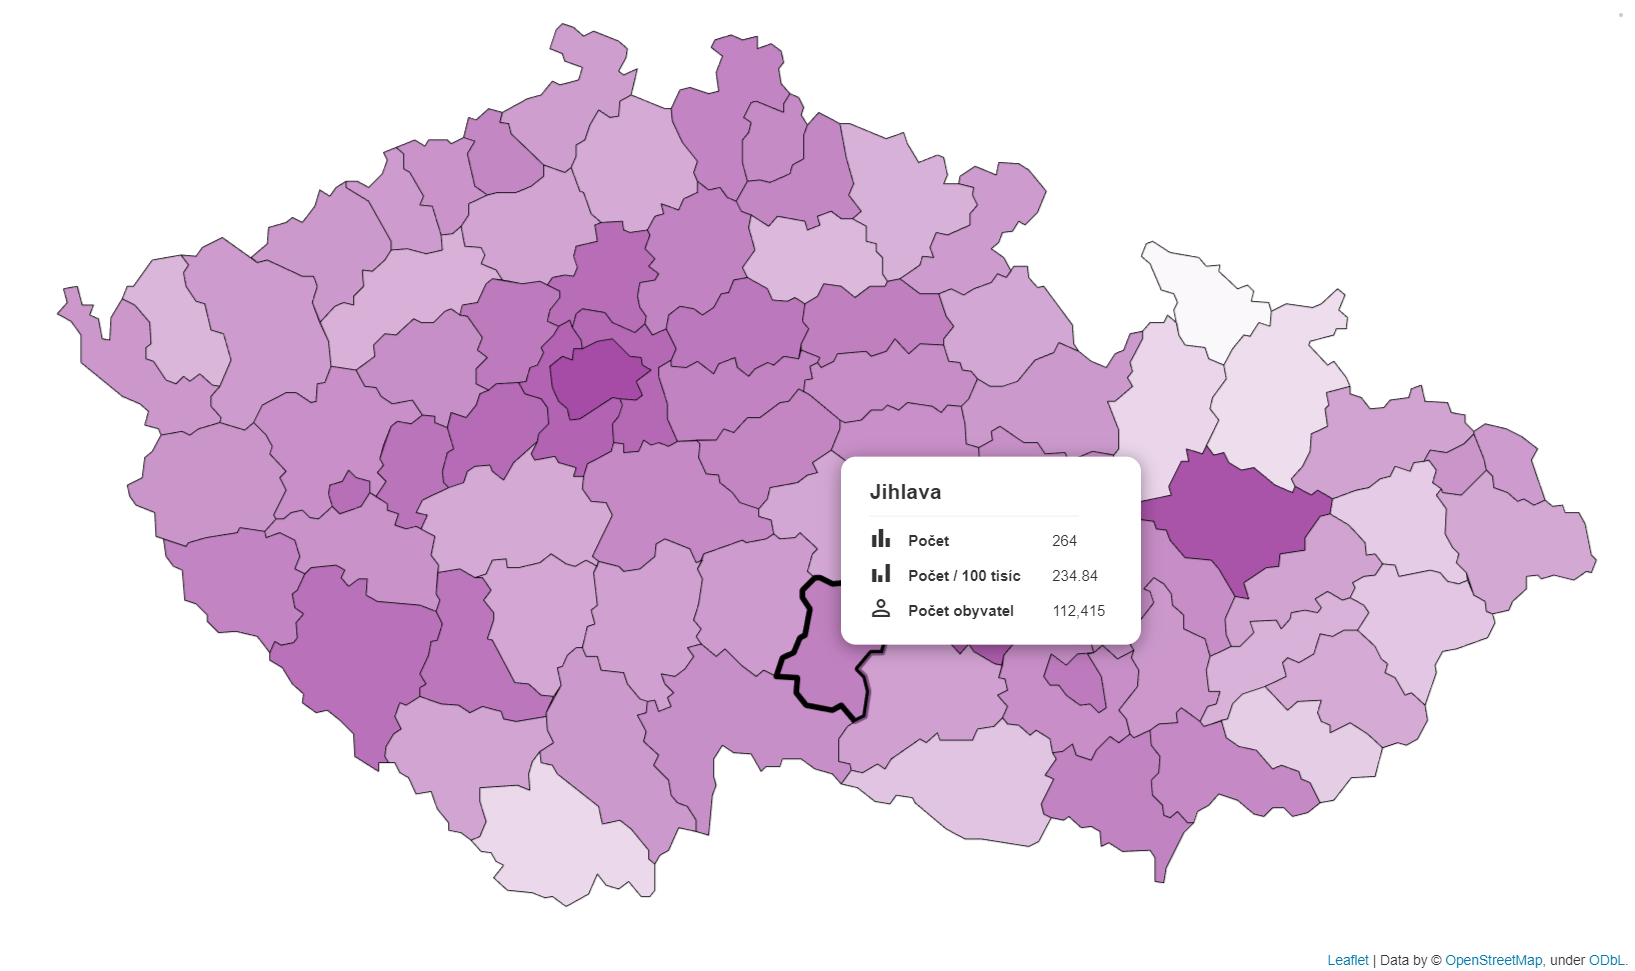
\includegraphics[width=0.47\textwidth]{Pictures/showcase5d.png} \\
(c) Zaznamenaná úmrtí & (d) Provedené PCR testy \\[6pt]
\end{tabular}
\caption{Ukázka využití aplikace č. 1}
\label{showcase5}
\end{figure}

\clearpage

\subsubsection*{Nalezení dne s~největším přírůstkem nakažených na 100 tisíc obyvatel}
\label{uisample}

V~případě hledání dne s~největším přírůstkem nakažených je vhodné stáhnout všechna dostupná data a~poté zobrazit graf. Skvělým vodítkem, jak nalézt den s~největším přírůstkem nakažených, je zkoumat výkyvy nakažených v~grafu. Když si například rozklikneme okres Praha, tak na grafu spatříme, že nejsilnější vlna probíhala od začátku zimy roku 2021 po začátek jara roku 2022. Pro usnadnění práce si můžeme časové okno přizpůsobit tomuto časovému rozmezí a~aktualizovat data. Po stažení nových dat můžeme nalézt maximální nalezenou hodnotu v~levém spodním okně u~škály. Je nutné nastavit vyobrazená data na \emph{Nové případy} a~škálovat podle přepočtu na 100 tisíc obyvatel. Dozvíme se, že nejvyšší přírůstek je 1086. Abychom našli přesný den, je možné si graf rozkouskovat a~sledovat jeho menší části. Největší výkyv byl spatřen od poloviny ledna 2022 do konce ledna 2022. Při přejetí myší po hodnotách grafu lze zjistit o~který konkrétní den se jedná. Poté je doporučeno si časové okno opět přizpůsobit a~také škálovat hodnoty podle maximální nalezené hodnoty. Díky animaci zjistíme, že největší nalezený přírůstek byl právě v~okrese Mladá Boleslav dne 1. února 2022. Výsledek lze vidět na obrázku \ref{fig:Showcase1}.

\begin{figure}[h]
	\centering
	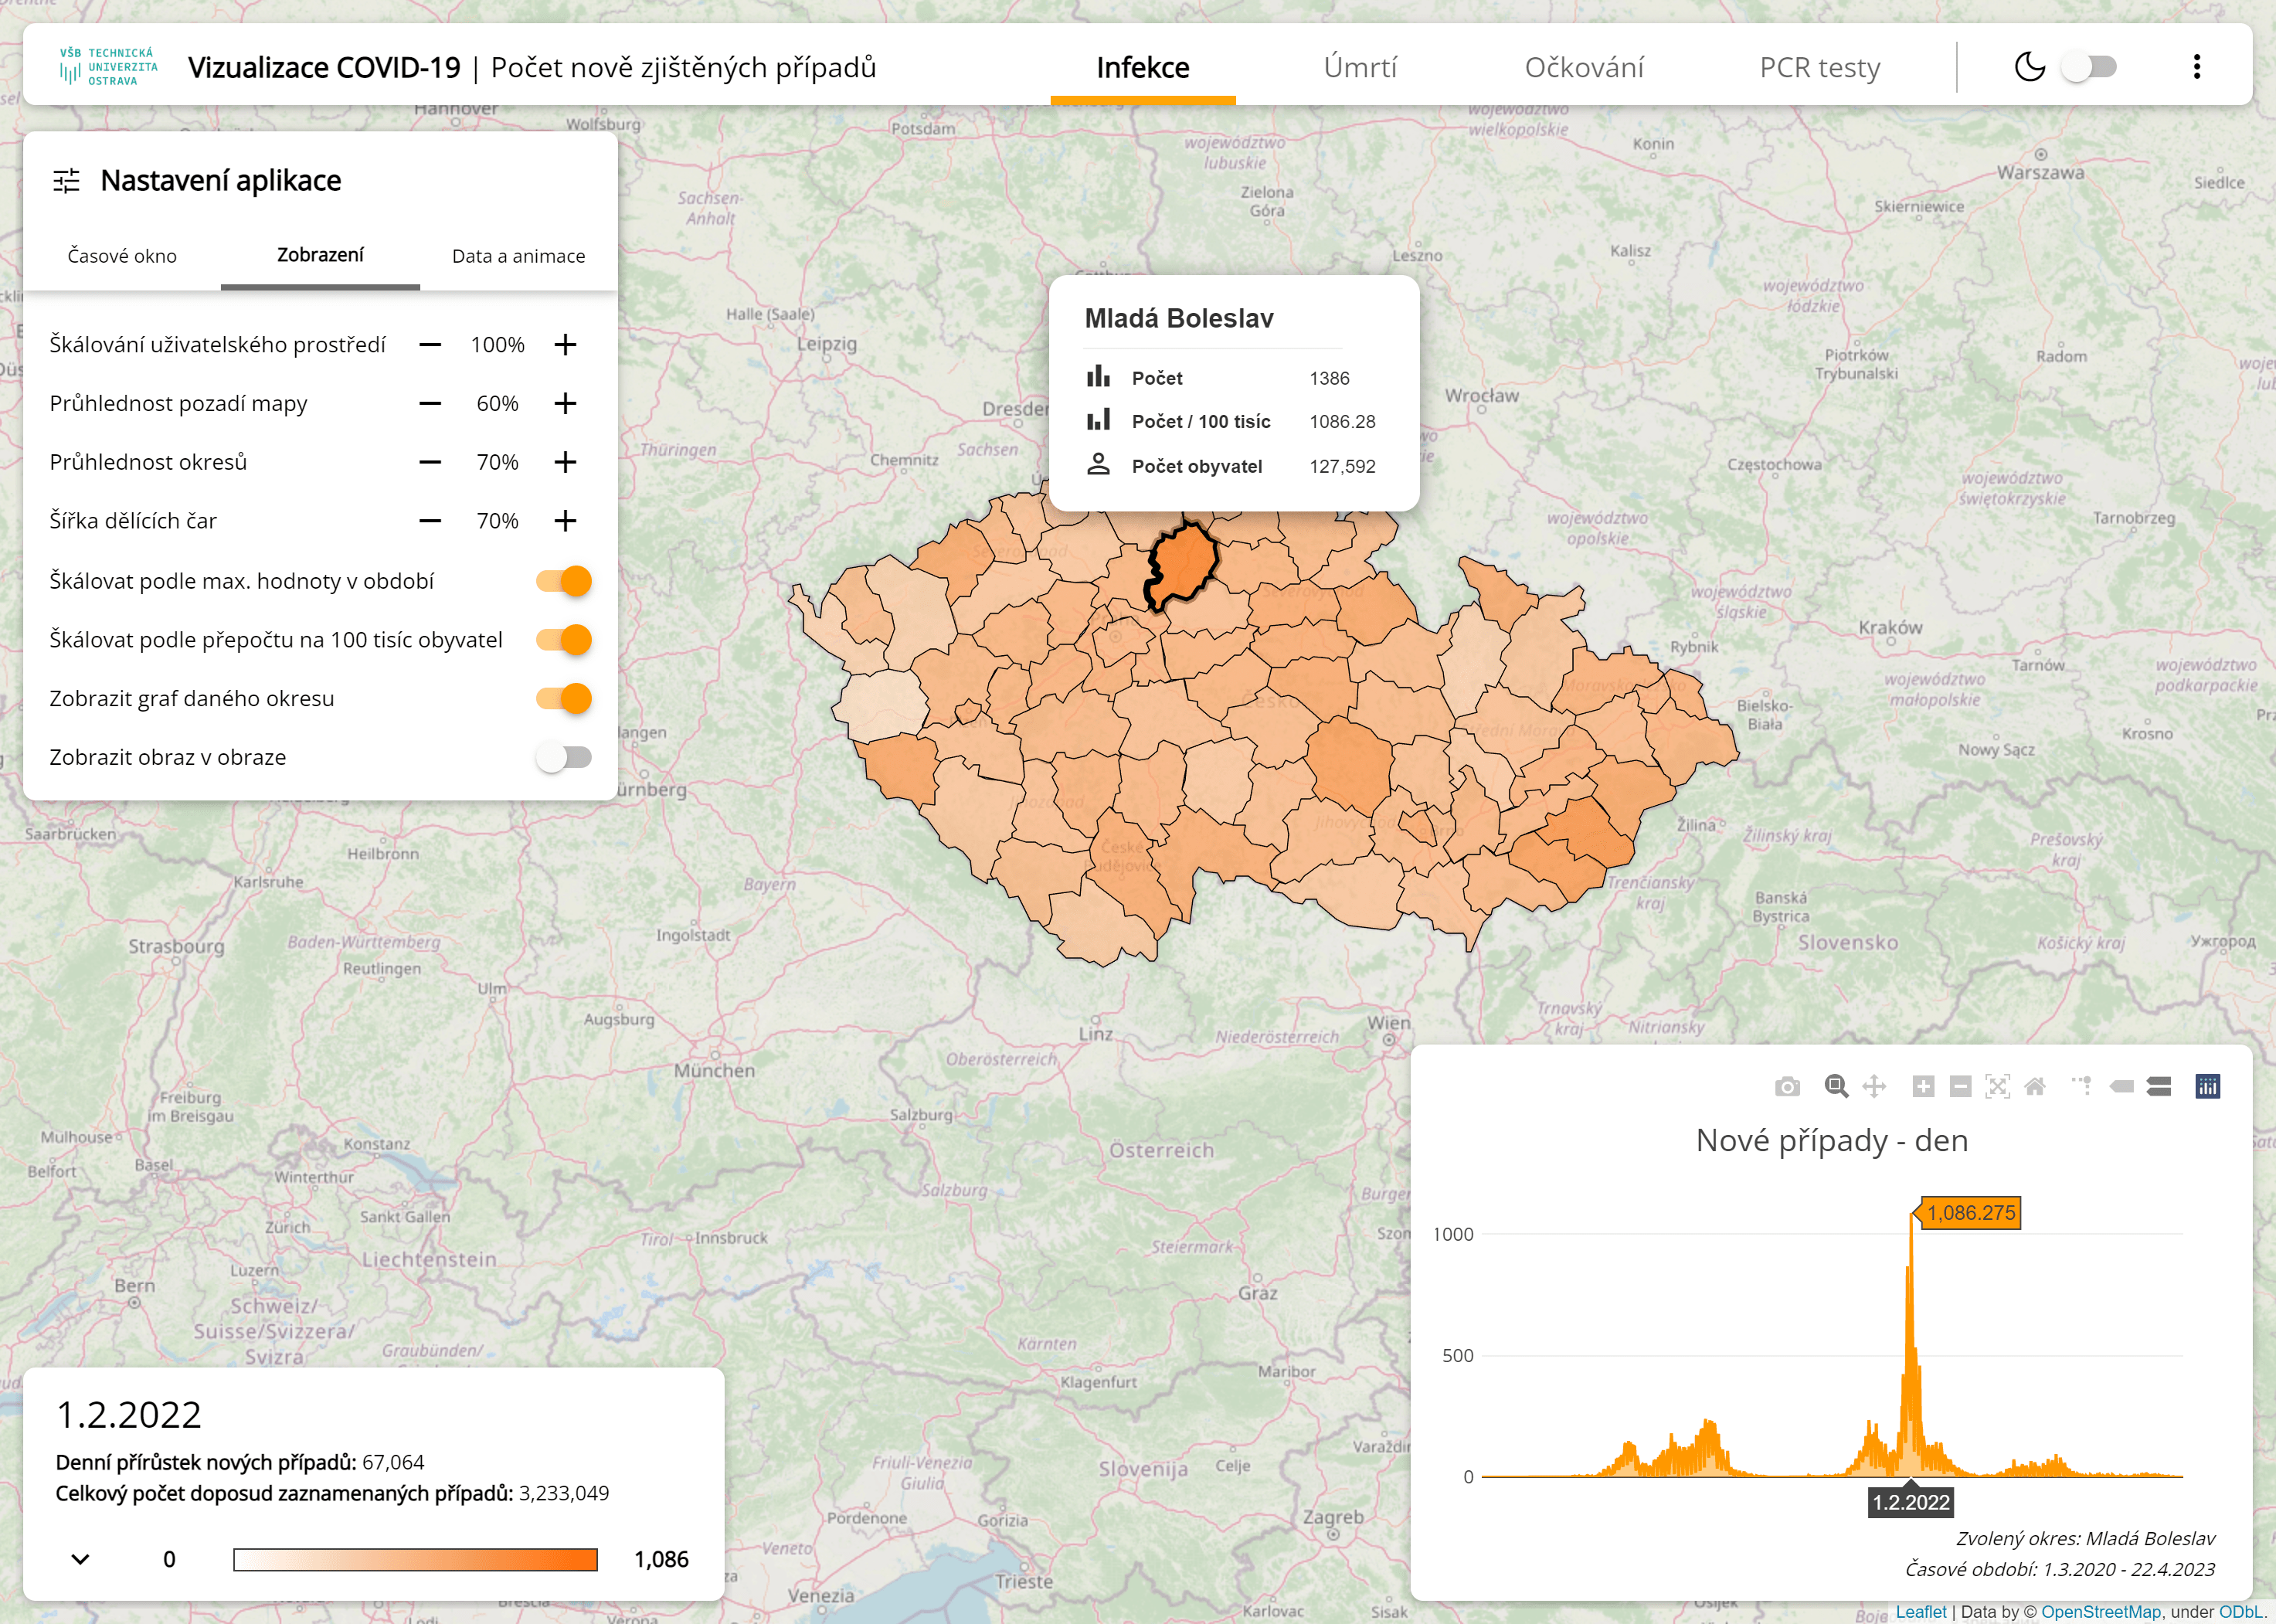
\includegraphics[width=1\textwidth]{Pictures/showcase2.png}
	\caption{Ukázka využití aplikace č. 2}
	\label{fig:Showcase1}
\end{figure}

\clearpage

\subsubsection*{Zkoumání průběhu očkování v~okrese}

Dataset očkování obsahuje informace o~každé ze čtyř dávek očkování pro všechny okresy. Aplikace je tudíž schopna vyobrazit průběh jednotlivých dávek ve zvolených okresech, lze například spatřit kdy se začalo očkovat danou dávkou. Tento průběh je nejlépe vidět na grafech. Pro zobrazení těchto grafů je nutné stáhnout veškerá data a~poté zvolit okres (na obrázcích \ref{showcase3} je zvolený okres Ostrava-město). Jakmile je okres zvolen, stačí zobrazit graf v~nastavení a~vybrat data s~danou dávkou. Pro zjištění konkrétního dne je možné myší \enquote{přejet} přes hodnotu v~grafu, tím jsme také schopni zjistit, kdy se přibližně začalo danou dávkou očkovat ve vybraném okrese.
\vspace*{0.5in}
\begin{figure}[h]
\centering
\begin{tabular}{cc}
  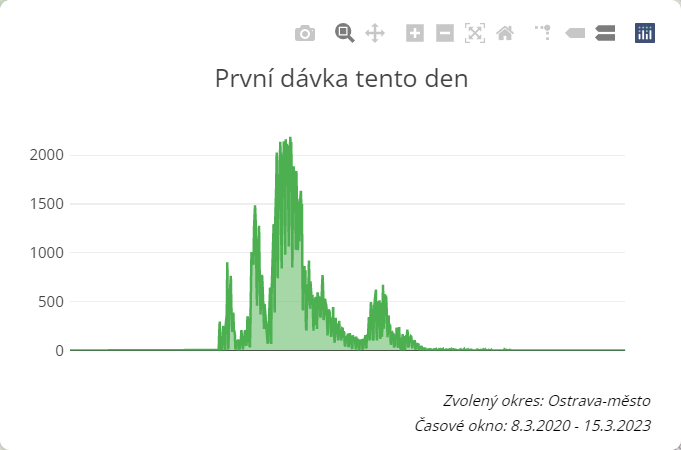
\includegraphics[width=0.47\textwidth]{Pictures/showcase3a.png} &   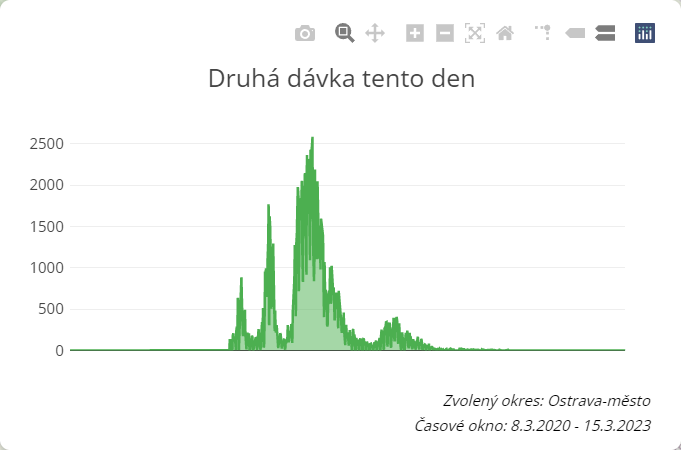
\includegraphics[width=0.47\textwidth]{Pictures/showcase3b.png} \\
(a) První dávka & (b) Druhá dávka \\[6pt]
 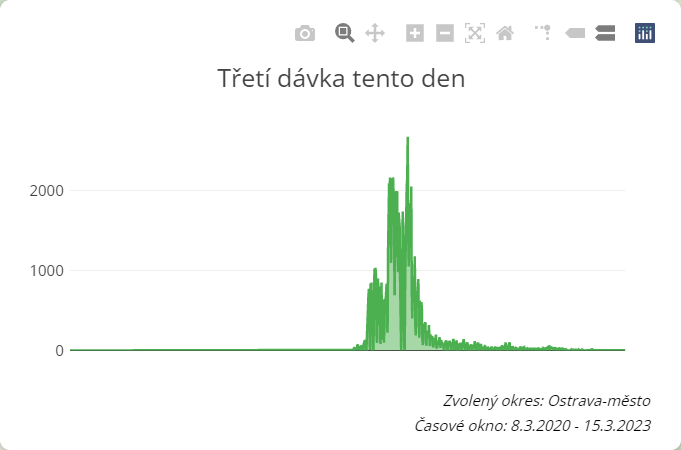
\includegraphics[width=0.47\textwidth]{Pictures/showcase3c.png} &   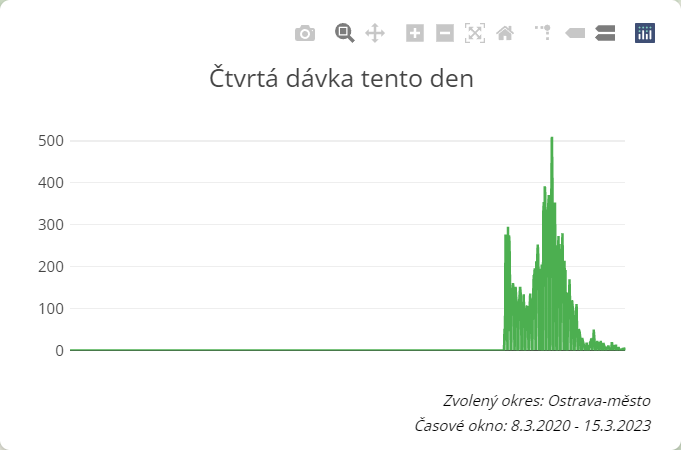
\includegraphics[width=0.47\textwidth]{Pictures/showcase3d.png} \\
(c) Třetí dávka & (d) Čtvrtá dávka \\[6pt]
\end{tabular}
\caption{Ukázka využití aplikace č. 3}
\label{showcase3}
\end{figure}

\clearpage

\subsubsection*{Zkoumání souvislostí mezi datasety}

Zkoumání souvislostí je jedna z~výhod, kterou poskytuje část aplikace zvaná obraz v~obraze (viz. \ref{pip}). Díky dodatečnému oknu lze zobrazit dvě mapy České republiky zároveň s~rozdílnými vyobrazenými datasety. Na obrázku \ref{fig:Showcase4} vidíme hlavní mapu zobrazující denní přírůstek infikovaných a~v~menší mapě lze vidět počet provedených PCR testů. Na těchto dvou mapách lze spatřit souvislost mezi těmito datasety. Na místech, kde se provádělo hodně PCR testů, často přibyl značný počet infikovaných. Avšak ne vždy musí být toto pravda, v~některých okresech tomu tak není. Tento fakt může naznačovat, že PCR testy mají velkou šanci na odhalení koronaviru v~jedinci a~tudíž se z~něj stává infikovaný - nový případ.

\vspace*{0.5in}
\begin{figure}[h]
	\centering
	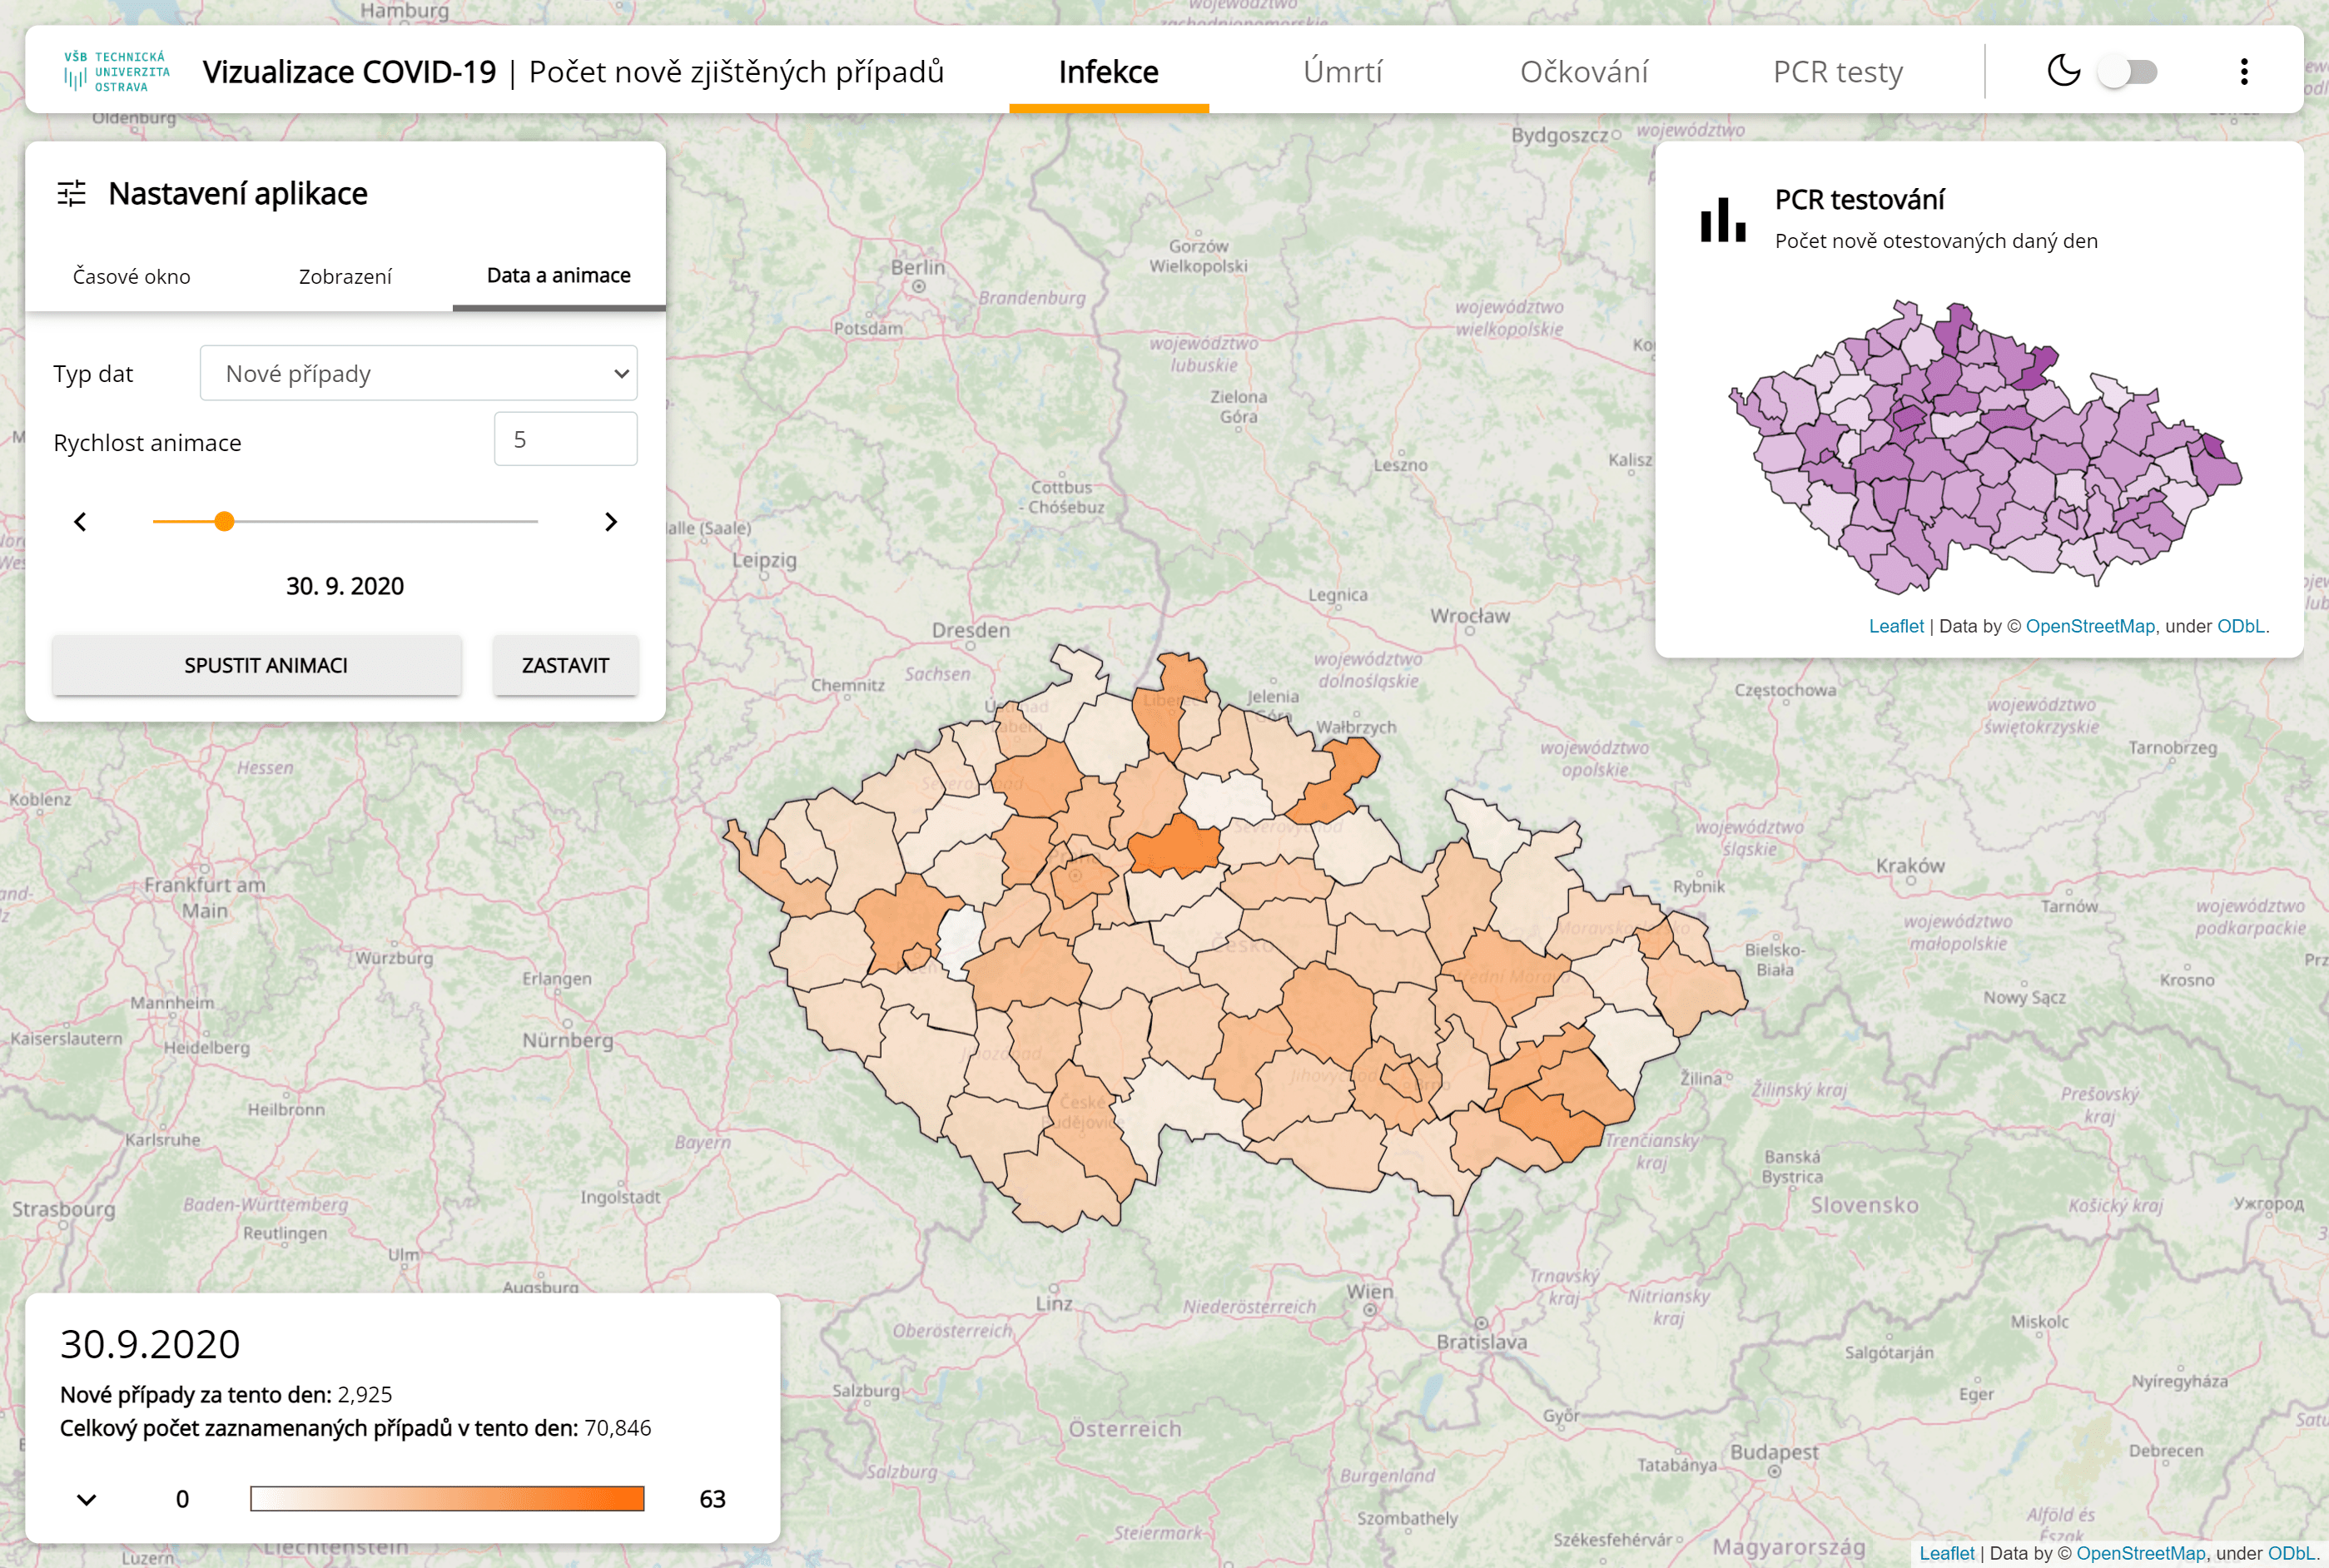
\includegraphics[width=1\textwidth]{Pictures/showcase4.png}
	\caption{Ukázka využití aplikace č. 4}
	\label{fig:Showcase4}
\end{figure}

\endinput

\chapter{Závěr}

Hlavním cílem práce bylo zvizualizovat data onemocnění covid-19 v~rámci okresů České republiky. Po zkoumání různých možností se rozhodlo, že se bude jednat o~webovou aplikaci, ke které bude uživatel přistupovat pomocí webového prohlížeče. Na úvod bylo popsáno onemocnění covid-19 společně s~dostupnými daty a~poté byly detailně popsány veškeré důležité části aplikace. Při vyvíjení aplikace bylo získáno mnoho zajímavých zkušeností a~poznatků s~obecným fungováním webových aplikací a~frameworkem Django, jež byl pro realizaci práce použit.

Cíl práce byl splněn a~aplikace byla úspěšně vytvořena. Výsledkem je plnohodnotná webová aplikace, která poskytuje uživateli širokou škálu dat, jež lze zvizualizovat na interaktivní mapě ČR rozdělené na okresy. Pro konkrétní potřeby uživatele jsou dostupná různá přizpůsobení mapy i~škálování dat. V~porovnání s~existujícími aplikacemi je nově vytvořená aplikace jediná, která dokáže plně vizualizovat covidová data formou interaktivní mapy ČR rozdělené na okresy a~je schopná si vizualizaci přizpůsobit ať už z~hlediska dat, času, nebo vzhledu. Navíc obsahuje dodatečné funkce jako např. obraz o~obraze.

Stále existují cesty, jak aplikaci obohatit. Užitečným doplňkem by bylo přizpůsobení stahovaných dat nebo rozšíření o~nové rozdělení mapy na kraje. V~budoucnu by bylo vhodné aplikaci připravit na nasazení na server. Předpokládá se, že se bude aplikace chovat odlišně, protože by běžela 24/7 na serveru a~občas by mohla být pod tlakem více připojených uživatelů. 

\section{Co se zdařilo a~nezdařilo}

\subsubsection*{Vizualizace covidových dat v~okresech}

V~této aplikaci se kladl velký důraz na samotnou vizualizaci dat. Výsledná vizualizace se velice zdařila a~poskytuje uživateli svobodu přizpůsobení jeho vlastnímu použití. Jádrem celé vizualizace je mapa, která je plně interaktivní a~funguje i~na dotykových obrazovkách. Důležitou součástí je i~animace, kde dochází k~prolínání dní za sebou ve zvoleném časovém okně. Vzhledem k~možnostem vizualizace a~jejímu přizpůsobení považuji tento způsob jako velice zdařilý.

\subsubsection*{Vzhled aplikace na straně klienta}

Je důležité příchozího uživatele oslovit a~ne jej odradit od používání aplikace. Proto je využito moderní uživatelské rozhraní, které je inspirované Material Designem. Samotné rozhraní obsahuje přívětivé animace, moderní minimalistický design a~měnící se barevné schéma vzhledem k~vybranému datasetu. Rozhraní také poskytuje tmavý režim pro komfort uživatele a~schopnost skrýt určitá okna. Podle zkušeností používání této aplikace lze říci, že prostředí je přehledné a~nelze se v~něm jednoduše ztratit.

\subsubsection*{Dostupná data}

Veškerá užitá data pochází z~MZČR a~ČSÚ. API od Ministerstva zdravotnictví poskytuje širokou škálu dat, kterou lze využít k~různým analýzám a~vizualizacím. Problém ale nastává v~tom, že většina těchto dat není použitelná pro tuto aplikaci. Značná část těchto dat se vztahuje buď na celou Českou republiku nebo kraje, pouze malá část dat obsahuje informace o~okresech. S~některými využitými daty ale nastal problém a to u infekcí, kde nelze z~využitého datasetu \emph{obce} vyčíst počet aktivních případů. Nové případy v~okrese se počítají součtem nových případů v~obcích v~daném okrese a~celkový sečtený počet pro okres odpovídá správnému výsledku. Stejný způsob ale nelze použít pro aktivní případy neboť výsledek často bývá nesmyslně mnohonásobně větší, než jaký má reálně být.

\subsubsection*{Aktuálnost dat}

Data, která poskytuje API Onemocnění aktuálně, jsou denně v~ranních hodinách aktualizována. Nejen, že přibyde nový den, ale velice často jsou aktualizovány i~předchozí dny, někdy i~týdny. Aplikace proto stahuje data vždy s~týdenním odstupem, aby se zajistila co největší aktuálnost dat. Poté již data neaktualizuje. Se současným API by bylo velice náročné data každodenně kontrolovat, zda došlo k~jejich změně. API je totiž limitované na 1000 požadavků na hodinu a~kontrolovat celou databázi by bylo výkonnostně náročné. Proto mohou být celkové výsledky vizualizace lehce nepřesné.

\endinput

% Seznam literatury
\printbibliography[nottype=book, title={Literatura}, heading=bibintoc]

\printbibliography[type=book, title={Bibliografie}, heading=bibintoc]

% Prilohy
\appendix
\chapter{Instalace a vytvoření projektu Djanga}

\begin{lstlisting}[style=bash,label=src:DjangoInstall,caption={Instalace a vytvoření projektu Djanga \cite{django-dokumentace}}]
# Zjištění verze Pythonu a instalace Pythonu verze 3.11 v Linuxu
$ python3 --version
$ sudo apt-get install python3.11

# Kontrola verze pip a instalace pip pro Python verze 3
$ pip --version
$ sudo apt-get install python3-pip

# Inicializace virtuálního prostředí 'my_venv' v současném adresáři
$ python3 -m venv my_venv

# Spuštění prostředí v systémech Linux/macOS
$ source my_venv/bin/activate

# Spuštění prostředí v systémech Windows
$ my_venv\Scripts\activate.bat

# Kontrola verze Djanga a instalace Djanga v Pythonu 3
$ python3 -m django --version
$ python3 -m pip install Django

# Instalace apscheduler v Pythonu 3
$ python3 -m pip install apscheduler



# Vytvoření nového projektu 'bp_project' v současném adresáři a vytvoření aplikace 'covid' v adresáři projektu
$ django-admin startproject bp_project
$ cd bp_project && python3 manage.py startapp covid
\end{lstlisting}

\endinput
\chapter{Vytvoření interaktivní mapy}

\begin{lstlisting}[language=Python,label=src:CreateMapFolium,caption={Vytvoření interaktivní mapy pomocí Folium}]
import folium
import json

# Vytvořit objekt mapy s nastavením defaultní polohy na mapě a přiblížením
map = folium.Map(location = [50, 15], zoom_start=8)

# Otevřít GeoJSON a uložit jeho obsah do proměnné
with open('geojson.json', 'r') as f:
    geojson = json.load(f)

# Vytvoření nové mapové vrstvy z GeoJSONu a přidání do vrstev mapy
folium.Choropleth(
    geo_data = geojson,
    columns = ["Okres", "Název"],
    key_on = 'feature.properties.name',
    fill_color = 'YlOrRd',
    fill_opacity = 0.7,
    line_opacity = 0.5).add_to(map)

# Základní styl GeoJSON objektů na mapě
style = lambda x: {'fillColor': '#000000', 
                   'color':'#000000', 
                   'fillOpacity': 0.5, 
                   'weight': 0.5}

# Vytvoření vyskakovacího okna na mapě společně s "hoverem"
features = folium.features.GeoJson(
    geojson,
    style_function = style, 
    control = False,
    tooltip = folium.features.GeoJsonTooltip(
        fields = ['name'],
        aliases = ['Okres']),
    popup = folium.features.GeoJsonPopup(
        fields = ['name'],
        aliases = ['Okres'])
    )

# Přidání vyskakovacího okna společně s "hoverem" do mapy
map.add_child(features)

# Přidat vytvořenou mapu do ovládání vrstev
folium.LayerControl().add_to(map)

# Uložit interaktivní mapu do souboru
map.save('map.html')
\end{lstlisting}

\endinput
\chapter{Získání dat z~backendu aplikace}

\begin{figure}[h]
	\centering
	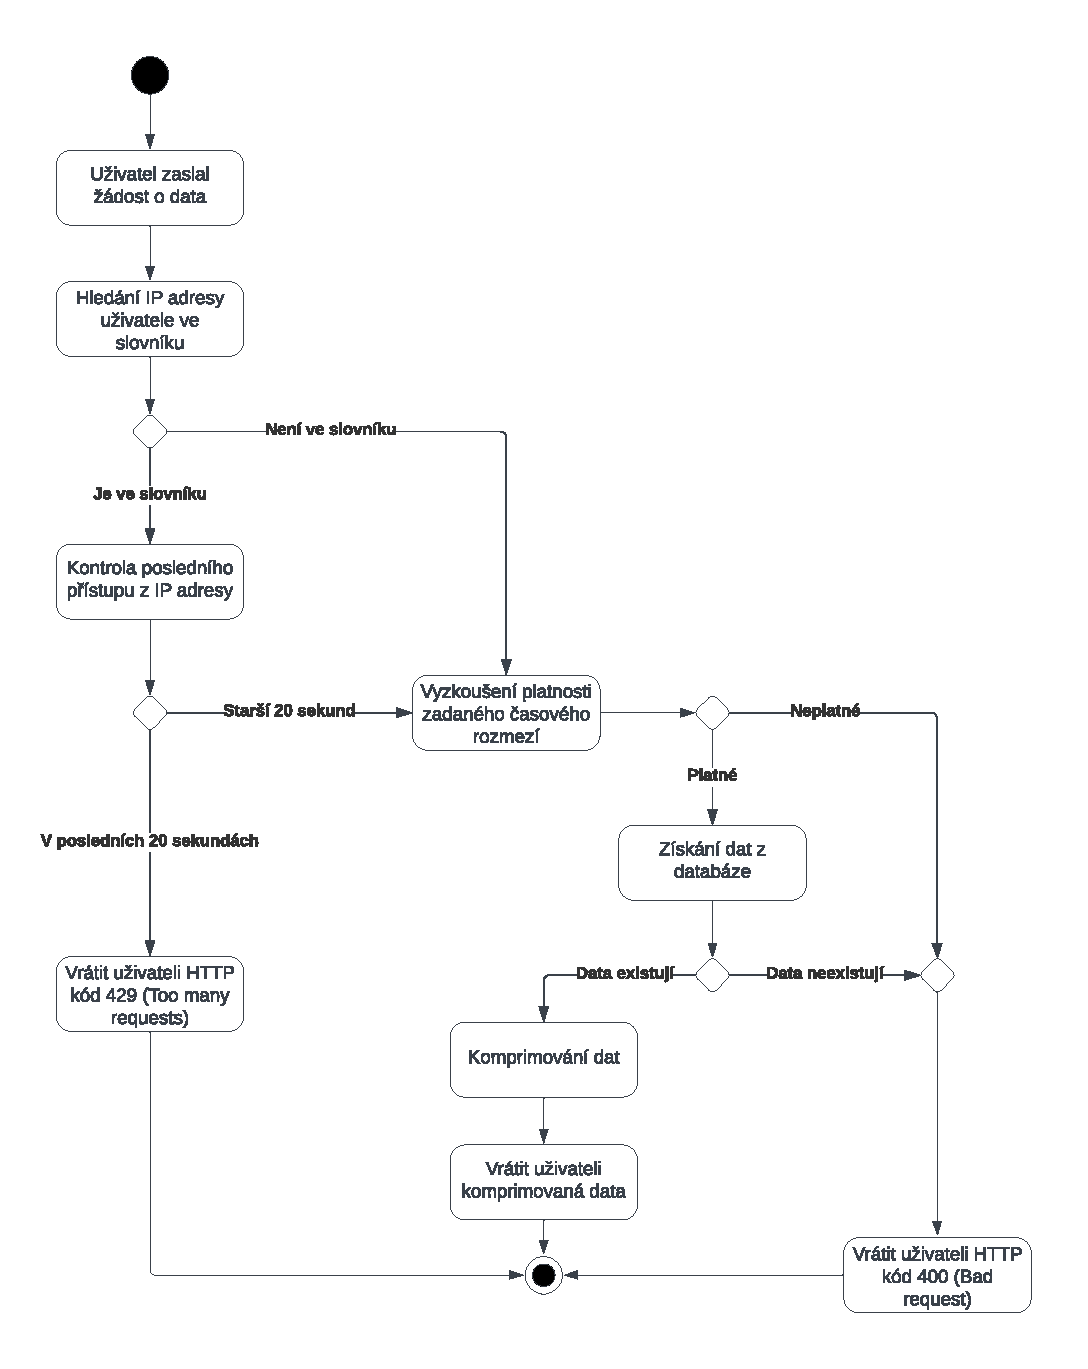
\includegraphics[width=0.65\textwidth]{Pictures/diagram1.pdf}
	\caption{Proces získání dat z~backendu aplikace znázorněný pomocí diagramu}
	\label{fig:Diagram1}
\end{figure}

\endinput
\chapter{Stažení a~ukládání nových dat do databáze}

\begin{figure}[h]
	\centering
	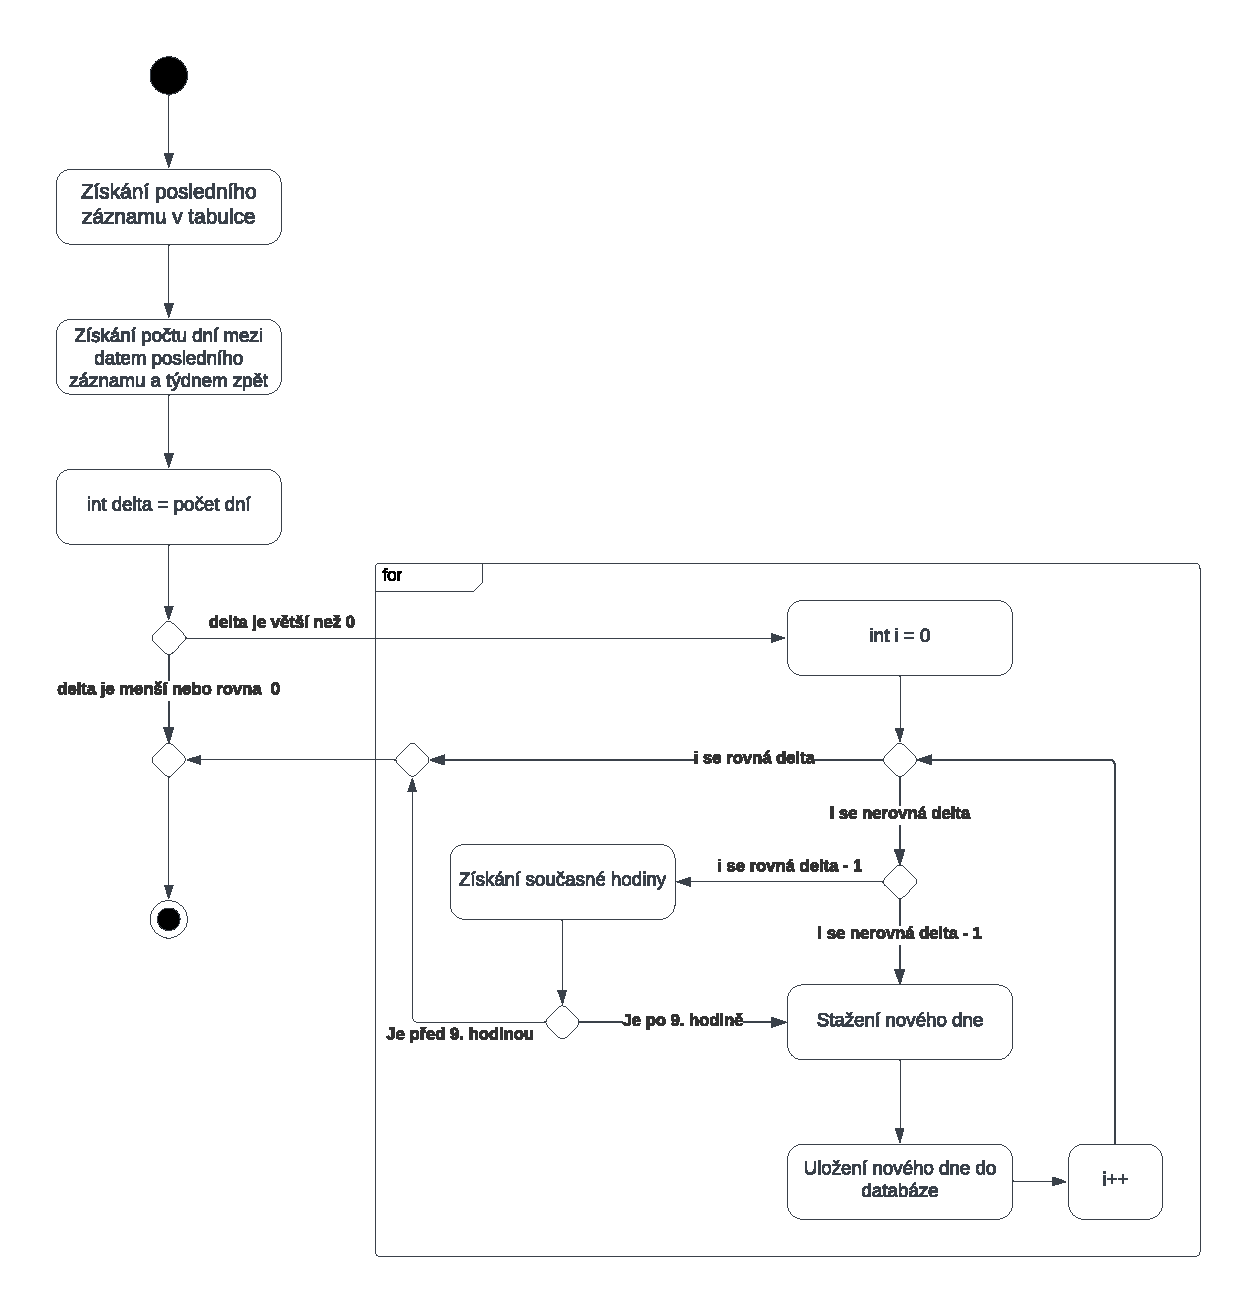
\includegraphics[width=0.75\textwidth]{Pictures/diagram2.pdf}
	\caption{Proces zjištění aktuálnosti dat v~databázi a~stažení nových dat z~API Onemocnění aktuálně - znázorněno diagramem}
	\label{fig:Diagram2}
\end{figure}

\endinput
\chapter{Use case diagram aplikace}

\begin{figure}[h]
	\centering
	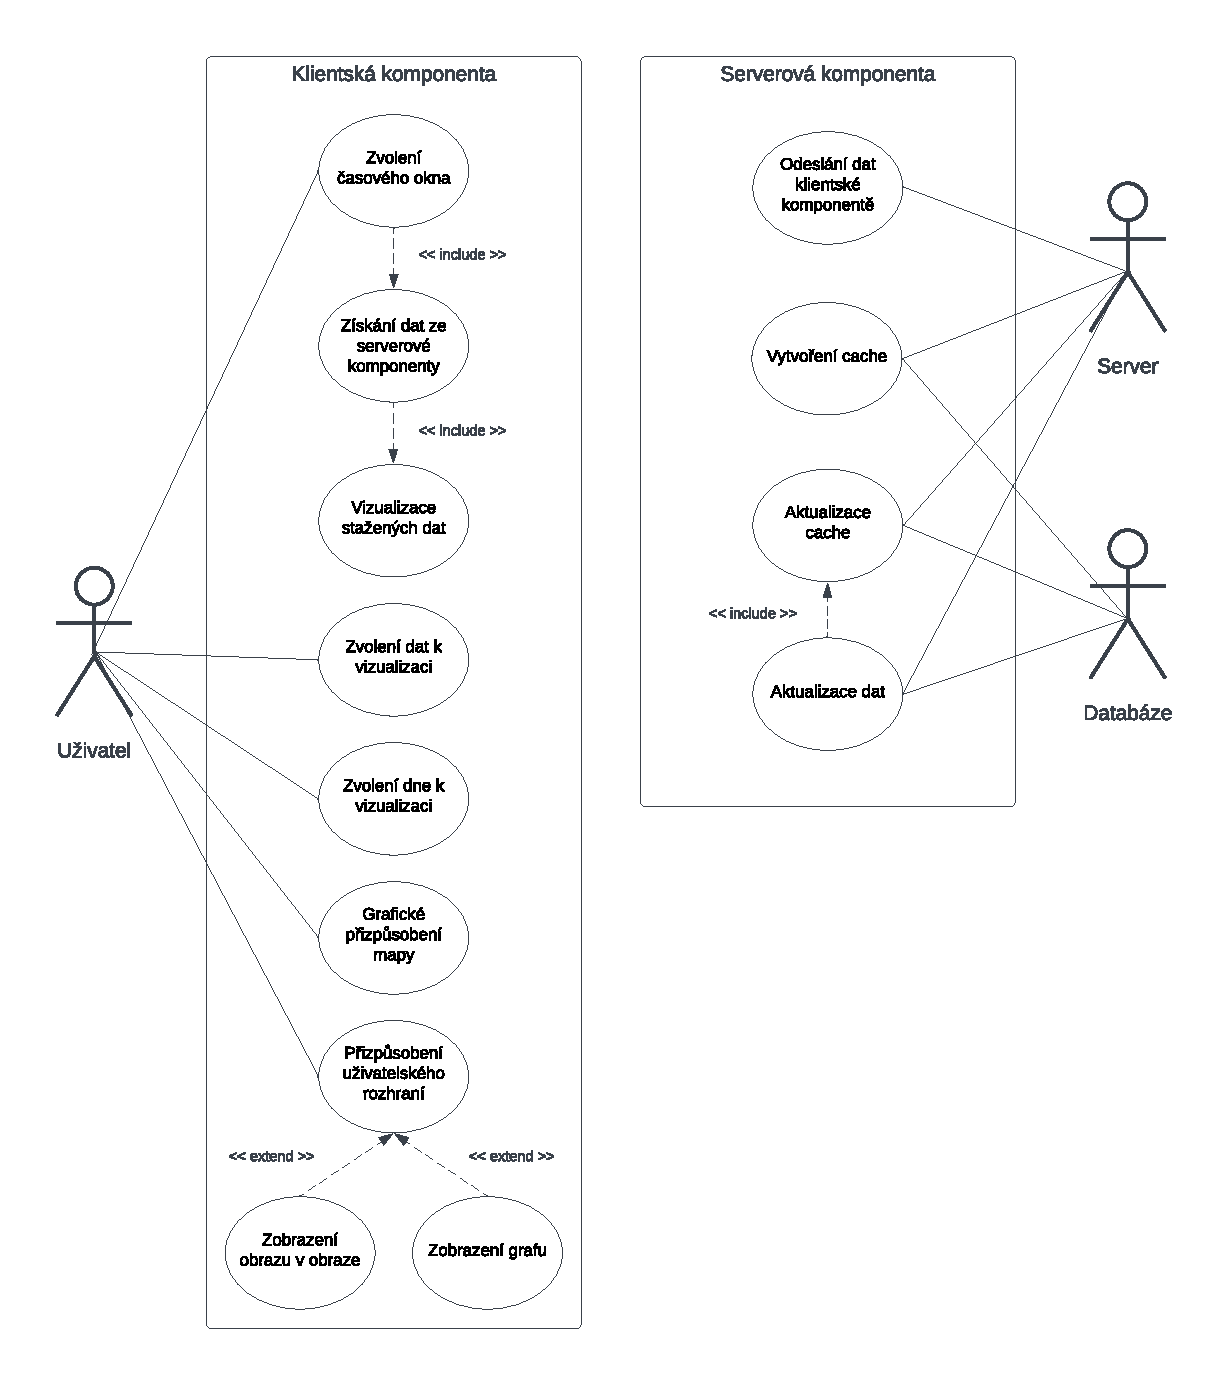
\includegraphics[width=1\textwidth]{Pictures/diagram3.pdf}
	\caption{Zachycení případů užití pomocí zjednodušeného use case diagramu}
	\label{fig:Diagram3}
\end{figure}

\endinput
\chapter{Třídní diagram backendu aplikace}

\begin{figure}[h]
	\centering
	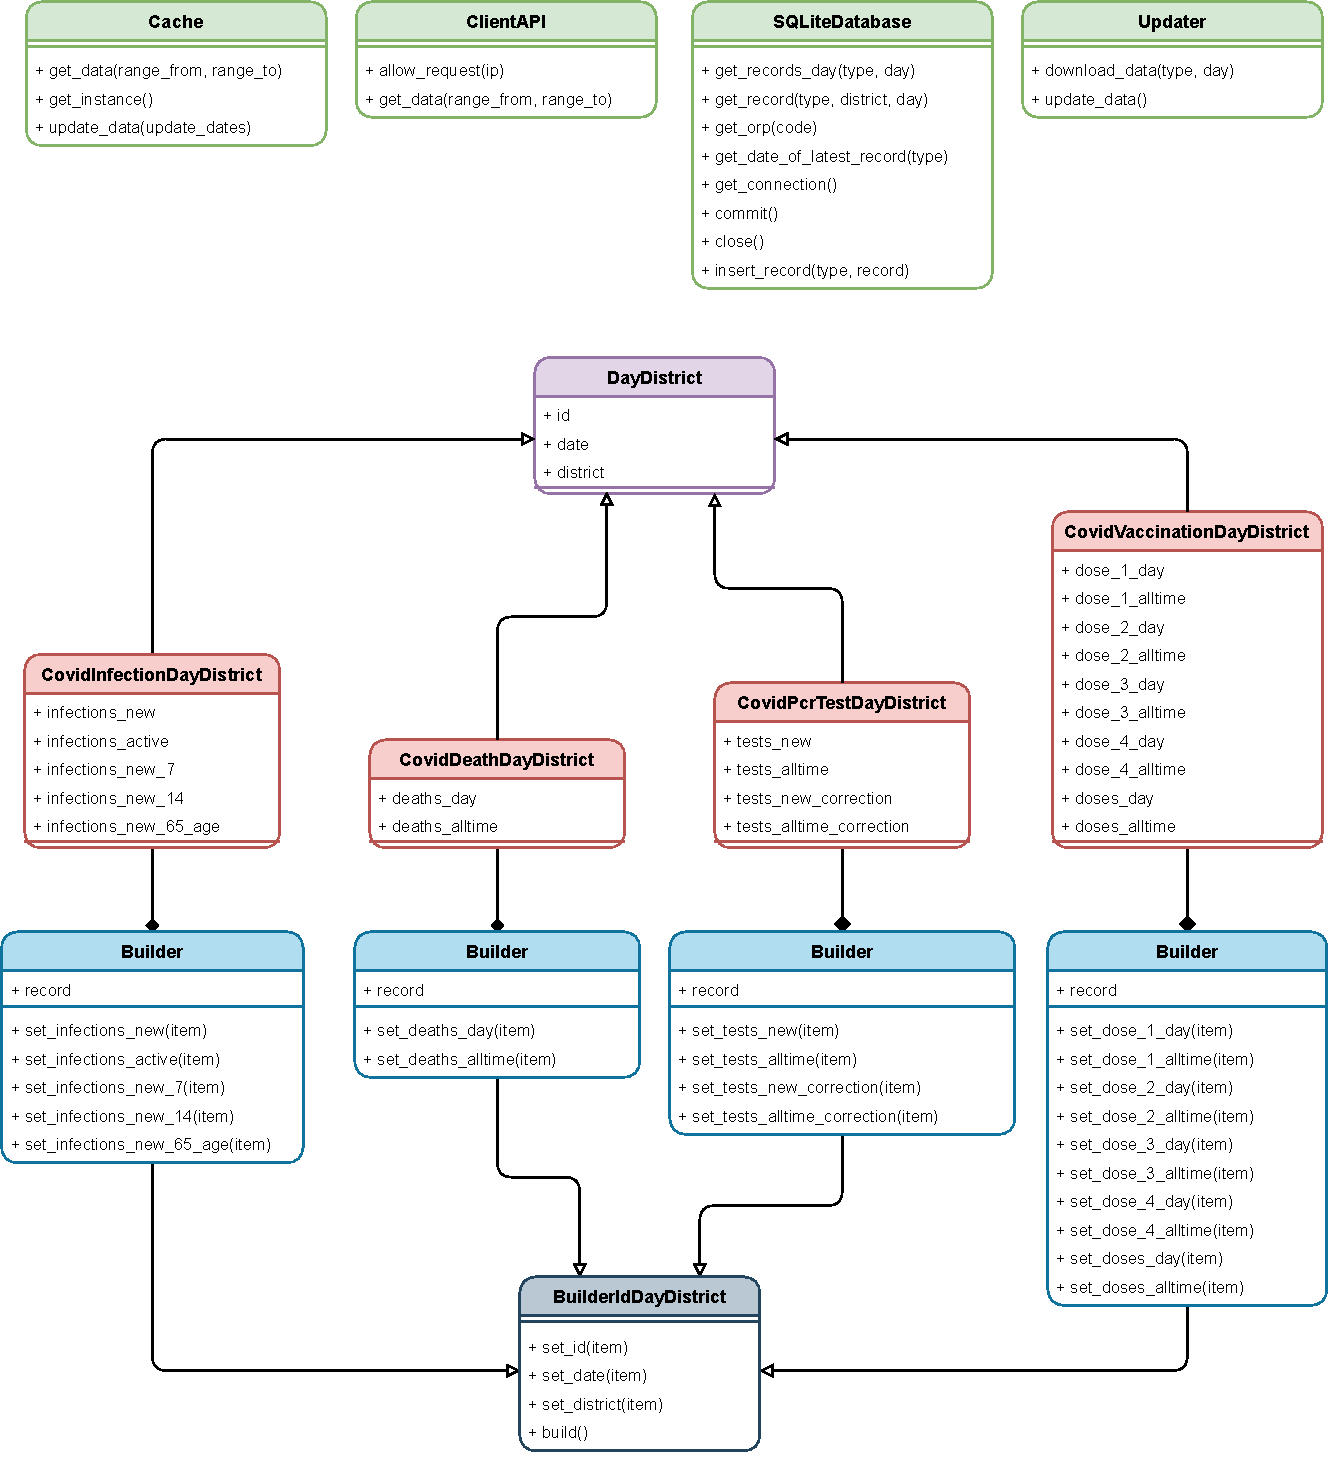
\includegraphics[width=1\textwidth]{Pictures/diagram4.pdf}
	\caption{Třídní diagram backendu aplikace}
	\label{fig:Diagram4}
\end{figure}

\endinput

\end{document}
